
%  PLEASE DO NOT REMOVE OR CHANGE THIS BLOCK
%  ===========================================================
%
%  A LaTeX Template for Typesetting Theses in Persian
%  By: Hamid Zarrabi-Zadeh
%  Source: https://github.com/zarrabi/thesis-template
%
%  License: Creative Commons Attribution 4.0
%  https://creativecommons.org/licenses/by/4.0/
%
%  Contributors: Ehsan Emamjomeh-Zadeh and Omid Gheibi
%  See the full list of contributors at GitHub.
%
%  ===========================================================


\documentclass[oneside,a4paper,12pt]{book}


% -------------------------------------------------------
%  Common Styles and Formattings
% -------------------------------------------------------

% 1. Import necessary packages
\usepackage{listings} % The main package for code listings
\usepackage{xcolor}   % Required for defining custom colors

\usepackage{amssymb,amsmath}
\usepackage[colorlinks,linkcolor=blue,citecolor=blue]{hyperref}
\usepackage[usenames,dvipsnames]{pstricks}
\usepackage{graphicx,subfigure,wrapfig}
\usepackage{geometry}
\usepackage[mathscr]{euscript}
\usepackage{multicol}
\usepackage{multirow}
\usepackage[figureposition=bottom,tableposition=top,font={small,bf},labelfont=bf]{caption}

\usepackage{algorithmicx,algorithm}

\usepackage[localise=on,extrafootnotefeatures]{xepersian}
\usepackage[noend]{algpseudocode}
\input{styles/alg-fa}


% -------------------- Page Layout --------------------


%\newgeometry{top=3cm,right=3cm,left=2.5cm,bottom=3cm,footskip=1.25cm}
\newgeometry{margin=1in,bottom=1.1in,footskip=.4in}

\renewcommand{\baselinestretch}{1.4}
\linespread{1.6}
\setlength{\parskip}{0.45em}

%\fancyhf{}
%\rhead{\leftmark}
%\lhead{\thepage}

\sloppy


% -------------------- Default Font --------------------

\settextfont[
Scale=1.09,
Extension=.ttf, 
Path=styles/fonts/,
BoldFont=XB NiloofarBd,
ItalicFont=XB NiloofarIt,
BoldItalicFont=XB NiloofarBdIt
]{XB Niloofar}

\setdigitfont[
Scale=1.09,
Extension=.ttf, 
Path=styles/fonts/,
BoldFont=XB NiloofarBd,
ItalicFont=XB NiloofarIt,
BoldItalicFont=XB NiloofarBdIt
]{XB Niloofar}


% -------------------- Sharif Font --------------------

\newcommand{\shariffont}{
\settextfont[
Scale=1.4,
Extension=.ttf, 
Path=styles/fonts/,
BoldFont=Sharif1.3-SemiBold,
]{Sharif1.3-Regular}

\setdigitfont[
Scale=1.4,
Extension=.ttf, 
Path=styles/fonts/,
BoldFont=Sharif1.3-SemiBold,
]{Sharif1.3-Regular}
}

% -------------------- Styles --------------------


\SepMark{-}
\renewcommand{\labelitemi}{$\small\bullet$}



% -------------------- Environments --------------------


\newtheorem{قضیه}{قضیه‌ی}[chapter]
\newtheorem{لم}[قضیه]{لم}
\newtheorem{ادعا}[قضیه]{ادعای}
\newtheorem{مشاهده}[قضیه]{مشاهده‌ی}
\newtheorem{نتیجه}[قضیه]{نتیجه‌ی}
\newtheorem{مسئله}{مسئله‌ی}[chapter]
\newtheorem{تعریف}{تعریف}[chapter]
\newtheorem{مثال}{مثال}[chapter]


\newenvironment{اثبات}
	{\begin{trivlist}\item[\hskip\labelsep{\em اثبات.}]}
	{\leavevmode\unskip\nobreak\quad\hspace*{\fill}{\ensuremath{{\square}}}\end{trivlist}}

\newenvironment{alg}[2]
	{\begin{latin}\settextfont[Scale=1.0]{Times New Roman}
	\begin{algorithm}[t]\caption{#1}\label{algo:#2}\vspace{0.2em}\begin{algorithmic}[1]}
	{\end{algorithmic}\vspace{0.2em}\end{algorithm}\end{latin}}


% -------------------- Titles --------------------


\renewcommand{\listfigurename}{فهرست شکل‌ها}
\renewcommand{\listtablename}{فهرست جدول‌ها}
\renewcommand{\bibname}{\rl{{مراجع}\hfill}} 


% -------------------- Commands --------------------


\newcommand{\IN}{\ensuremath{\mathbb{N}}} 
\newcommand{\IZ}{\ensuremath{\mathbb{Z}}} 
\newcommand{\IQ}{\ensuremath{\mathbb{Q}}} 
\newcommand{\IR}{\ensuremath{\mathbb{R}}} 
\newcommand{\IC}{\ensuremath{\mathbb{C}}} 

\newcommand{\set}[1]{\left\{ #1 \right\}}
\newcommand{\seq}[1]{\left< #1 \right>}
\newcommand{\ceil}[1]{\left\lceil{#1}\right\rceil}
\newcommand{\floor}[1]{\left\lfloor{#1}\right\rfloor}
\newcommand{\card}[1]{\left|{#1}\right|}
\newcommand{\setcomp}[1]{\overline{#1}}
\newcommand{\provided}{\,:\,}
\newcommand{\divs}{\mid}
\newcommand{\ndivs}{\nmid}
\newcommand{\iequiv}[1]{\,\overset{#1}{\equiv}\,}
\newcommand{\imod}[1]{\allowbreak\mkern5mu(#1\,\,\text{پیمانه‌ی})}

\newcommand{\poly}{\mathop{\mathrm{poly}}}
\newcommand{\polylog}{\mathop{\mathrm{polylog}}}
\newcommand{\eps}{\varepsilon}

\newcommand{\lee}{\leqslant}
\newcommand{\gee}{\geqslant}
\renewcommand{\leq}{\lee}
\renewcommand{\le}{\lee}
\renewcommand{\geq}{\gee}
\renewcommand{\ge}{\gee}

\newcommand{\مهم}[1]{\textbf{#1}}
\renewcommand{\برچسب}{\label}

\newcommand{\REM}[1]{}
\renewcommand{\حذف}{\REM}
\newcommand{\لر}{\lr}
\newcommand{\کد}[1]{\lr{\tt #1}}
\newcommand{\پاورقی}[1]{\footnote{\lr{#1}}}



% -------------------- Dictionary --------------------


\newcommand{\dicalphabet}[1]{
\begin{minipage}{\columnwidth}
	\centerline{\noindent\textbf{\large #1 }}
	\vspace{.5em}
\end{minipage}
\nopagebreak[4]
}

\newcommand{\dic}[2]{\noindent  #2 \dotfill  \lr{#1} \\ }


% ------------------------------ Images and Figures --------------------------

\graphicspath{{figs/}}
\setlength{\intextsep}{0pt}  % for float boxes
\renewcommand{\psscalebox}[1]{}  % for LaTeX Draw

\newcommand{\floatbox}[2]
	{\begin{wrapfigure}{l}{#1}
	\centering #2 \end{wrapfigure}}

\newcommand{\centerfig}[2]
	{\centering\scalebox{#2}{\input{figs/#1}}}

\newcommand{\fig}[3]
	{\floatbox{#3}{\centerfig{#1}{#2}}}

\newcommand{\centerimg}[2]
	{\vspace{1em}\begin{center}\includegraphics[width=#2]{figs/#1}\end{center}\vspace{-1.5em}}

\NewDocumentCommand{\img}{m m o}
	{\begin{wrapfigure}{l}{\IfValueTF{#3}{#3}{#2}}
	\centering\includegraphics[width=#2]{figs/#1}\end{wrapfigure}}




% -------------------------------------------------------
%  Custom Definitions
% -------------------------------------------------------


\newcommand{\OPT}{\ensuremath{\mathop{\mathrm{OPT}}}}
\newcommand{\APX}{\ensuremath{\mathop{\mathrm{APX}}}}
\newcommand{\ALG}{\ensuremath{\mathop{\mathrm{ALG}}}}

% 2. Define colors for syntax highlighting
\definecolor{codegreen}{rgb}{0,0.6,0}
\definecolor{codegray}{rgb}{0.5,0.5,0.5}
\definecolor{codepurple}{rgb}{0.58,0,0.82}
\definecolor{backcolour}{rgb}{0.95,0.95,0.92}

% 3. Create a custom style for your code block
\lstdefinestyle{mystyle}{
    backgroundcolor=\color{backcolour},   
    commentstyle=\color{codegreen},
    keywordstyle=\color{magenta},
    numberstyle=\tiny\color{codegray},
    stringstyle=\color{codepurple},
    basicstyle=\ttfamily\footnotesize,
    breakatwhitespace=false,         
    breaklines=true,                 
    captionpos=b,                    
    keepspaces=true,                 
    numbers=left,                    
    numbersep=5pt,                  
    showspaces=false,                
    showstringspaces=false,
    showtabs=false,                  
    tabsize=2
}

% Set the default style for all listings
\lstset{style=mystyle}

\captionsetup[lstlisting]{labelformat=empty}


\begin{document}


% -------------------- Font Settings --------------------

%\shariffont  % برای استفاده از فونت شریف این خط را فعال کنید


% -------------------- Front Pages --------------------


% -------------------------------------------------------
%  Thesis Information
% -------------------------------------------------------

\newcommand{\ThesisType}
{پایان‌نامه}  % پایان‌نامه / رساله
\newcommand{\ThesisDegree}
{کارشناسی ارشد}  % کارشناسی / کارشناسی ارشد / دکتری
\newcommand{\ThesisMajor}
{مهندسی کامپیوتر}  % نام رشته / گرایش
\newcommand{\ThesisTitle}
{ﺣﻔﻆ ﺣﺮﻳﻢ ﺧﺼﻮﺻﻲ ﺗﻔﺎﺿﻠﻲ ﻣﺤﻠﻲ هنگاﻡ ﺍﻧﺘﺸﺎﺭ ﺩﺍﺩه‌هاﻱ ﺑﺎ ﺍﺑﻌﺎﺩ ﺑﺎﻻ ﻭ ﺩﺭ ﺣﺎﻝ ﺗﻐﻴﻴﺮ}  % عنوان پایان‌نامه / رساله
\newcommand{\ThesisAuthor}
{سید آرش ساعتچی}  % نام نویسنده
\newcommand{\ThesisSupervisor}
{دکتر رسول جلیلی}  % نام استاد راهنما
\newcommand{\ThesisAdvisor}
{استاد مشاور}  
\newcommand{\ThesisExaminer}
{دکتر مرتضی امینی}
\newcommand{\ThesisDate}
{شهریور 1404}
\newcommand{\ThesisDepartment}
{دانشکده مهندسی کامپیوتر}
\newcommand{\ThesisUniversity}
{دانشگاه صنعتی شریف}

% -------------------------------------------------------
%  English Information
% -------------------------------------------------------

\newcommand{\EnglishThesisDegree}{M.Sc.}

\newcommand{\EnglishThesisTitle}{Preserving Local Differential Privacy in the Release of High-Dimensional and Evolving Data}

\newcommand{\EnglishThesisAuthor}{Seyed Arash Saatchi}

\newcommand{\EnglishThesisSupervisor}{Dr. Rasool Jalili}

\newcommand{\EnglishThesisDate}{September 2025}

\newcommand{\EnglishThesisDepartment}{Department of Computer Engineering}

\newcommand{\EnglishThesisUniversity}{Sharif University of Technology}

\pagestyle{empty}
\include{front/template/title}

% info: برای درج هر یک از صفحات زیر، خط مربوطه را فعال کنید

%\include{front/template/besmellah}  % صفحه بسم الله
%\include{front/template/signatures}  % صفحه تصویب‌نامه
%\include{front/template/declaration}  % صفحه اظهارنامه

\pagestyle{plain}
\pagenumbering{tartibi}

\include{front/acknowledge}  % صفحه سپاس

% -------------------------------------------------------
%  Abstract
% -------------------------------------------------------


\شروع{وسط‌چین}
\مهم{چکیده}
\پایان{وسط‌چین}
\بدون‌تورفتگی

حریم خصوصی تفاضلی محلی یکی از رویکردهای پیشرو در حفاظت از داده‌های کاربران است که بدون اعتماد به کارپذیر، حریم خصوصی را تضمین می‌کند. این مفهوم با افزودن نوفه به داده‌های کاربران قبل از ارسال به سمت کارپذیر، امکان تحلیل داده‌ها را فراهم می‌سازد. این گزارش بر چالش‌های حفظ حریم خصوصی تفاضلی محلی در داده‌های با ابعاد بالا و در حال تغییر تمرکز دارد. از جمله چالش‌های اساسی در این زمینه، همبستگی میان ویژگی‌ها، افزایش حساسیت داده‌ها و مصرف سریع بودجه حریم خصوصی است که می‌تواند دقت و کارایی تحلیل‌های آماری را به شدت کاهش دهد. استفاده ایمن از این داده‌ها در حوزه‌هایی نظیر اینترنت اشیا، داده‌های سلامت و سیستم‌های نظارتی اهمیت بالایی دارد زیرا این داده‌ها معمولاً در تصمیم‌گیری‌های کلیدی و توسعه خدمات هوشمند مورد استفاده قرار می‌گیرند و حفظ حریم خصوصی کاربران در فرآیندها از اولویت بالایی برخوردار است. در این گزارش ضمن دسته‌بندی، مرور و مقایسه الگوریتم‌ها و کارهای پیشین راه‌کار جدیدی برای حل چالش داده‌های با‌ابعاد بالا و در حال تغییر ارائه شده است. این راهکار با بهره‌گیری از دو روش تبدیل هار و درهم‌سازی محلی، بودجه حریم خصوصی را به صورت بهینه تخصیص داده و موجب کاهش نوفه اضافی می‌شود. همچنین با مدیریت و کاهش دامنه داده‌ها، مشکلات مربوط به دامنه‌های بزرگ را حل کرده و دقت و کارایی فرآیندها را افزایش می‌دهد. در نهایت، نتایج این پژوهش چارچوبی عملی و کارآمد برای تحلیل داده‌های با‌ابعاد بالا و در حال تغییر فراهم می‌کند که می‌تواند به عنوان یک ابزار کاربردی در سیستم‌های مبتنی بر داده به کار گرفته شود.

\پرش‌بلند
\بدون‌تورفتگی \مهم{کلیدواژه‌ها}: 
ﺣﺮﻳﻢ ﺧﺼﻮﺻﻲ ﺗﻔﺎﺿﻠﻲ ﻣﺤﻠﻲ، ﺩﺍﺩﻩﻫﺎﻱ ﺩﺭ ﺣﺎﻝ ﺗﻐﻴﻴﺮ، ﺩﺍﺩﻩﻫﺎﻱ ﺑﺎ ﺍﺑﻌﺎﺩ ﺑﺎﻻ، تبدیل هار، درهم‌سازی محلی
\صفحه‌جدید



% -------------------- Table of Contents --------------------

\tableofcontents \newpage
\listoftables \newpage
\listoffigures \newpage


% -------------------- Chapters --------------------

\pagenumbering{arabic}


\فصل{مقدمه}

در دنیای امروز که داده‌ها به بخش مهمی از تصمیم‌گیری‌ها و توسعه سیستم‌های اطلاعاتی تبدیل شده‌اند، حفاظت از حریم خصوصی افراد از اهمیت بالایی برخوردار است. حریم خصوصی تفاضلی\پانویس{Differential Privacy} به عنوان یک چارچوب ریاضی، رویکرد نوینی را برای جلوگیری از افشای اطلاعات حساس افراد در تحلیل داده‌ها ارائه می‌دهد.

انتشار داده‌ها بر مبنای حریم خصوصی تفاضلی اخیراً توجه زیادی را به خود جلب کرده و همچنین الگوریتم‌های متنوعی برای بهبود آن ارائه شده‌است. تعریف ریاضی حریم خصوصی تفاضلی بیان می‌کند که نتیجه هر تحلیل آماری روی داده‌ها، چه شما در آن شرکت کنید و چه نه، یکسان باشد. یعنی اطلاعاتی که از داده‌ها استخراج می‌شود، به گونه‌ای طراحی شده‌است که هیچ فردی نتواند از مشارکت یا عدم مشارکت خود، آسیب یا مزیتی دریافت کند. به عبارت دیگر، حریم خصوصی تفاضلی تضمین می‌کند که داده‌های فردی در برابر تحلیل‌های جمعی محافظت می‌شوند و هیچ گونه اطلاعات خاصی درباره افراد در معرض خطر قرار نمی‌گیرد. این ویژگی باعث می‌شود که افراد با اطمینان بیشتری در تحلیل‌های آماری شرکت کنند.

طی چند سال گذشته، راه حل‌هایی ارائه شده‌است تا هر کاربر بتواند ابتدا روی داده‌های خود نوفه\پانویس{Noise} ایجاد کرده و سپس آن‌ها را به سمت کارپذیر ارسال کند. به این راه حل‌ها، الگوریتم‌های حریم خصوصی تفاضلی\پانویس{Local Differential Privacy} محلی گفته می‌شود. در این الگوریتم‌ها، حتی با وجود غیر‌قابل اعتماد بودن کارپذیر، حریم خصوصی کاربران محفوظ باقی می‌ماند. لازم به ذکر است در انتشار داده‌های خصوصی با ابعاد بالا\پانویس{High Dimensional} با چالش‌هایی مانند روابط پیچیده بین ویژگی‌ها، پیچیدگی محاسباتی بالا و پراکندگی داده‌ها روبه‌رو هستیم. راه حل‌های موجود که با تمرکز روی داده با ابعاد پایین ارائه شده‌اند، بودجه حریم خصوصی را بین همه ویژگی‌ها تقسیم می‌کنند. با پیاده‌سازی این راه حل‌ها روی داده با ابعاد بالا، نوفه در مقیاس بالا تولید شده و سیستم کارایی خود را از دست می‌دهد. از طرفی یکی دیگر از چالش‌های حفظ حریم خصوصی تفاضلی، کار روی داده‌های در حال تغییر\پانویس{Evolving Data} است. یک نمونه بارز در چنین مسائلی، نظارت برخط\پانویس{Online} روی برنامه‌های نرم‌افزاری و گزارش عملکرد آن‌ها است، زیرا داده‌های ارسالی همواره در حال تغییر هستند. پروتکل‌های فعلی جمع‌آوری داده‌ها می‌توانند حریم خصوصی تفاضلی را در داده‌های با دامنه تغییرات محدود ارضا کنند. در نتیجه برای دامنه‌های بزرگ، مانند دامنه تغییرات داده‌ها در اینترنت‌اشیاء\پانویس{Internet of Things}، ناکارآمد خواهند بود. هدف از این پژوهش ارائه راهکاری به منظور حفظ حریم خصوصی کاربران در هنگام انتشار داده‌ها با ابعاد بالا و در حال تغییر است. به منظور ارزیابی عملکرد و کارایی این الگوریتم، ما به تحلیل و محاسبه فراوانی داده‌ها پرداخته و مقدار خطای بدست آمده را با خروجی سایر الگوریتم‌های موجود مقایسه می‌کنیم. این مقایسه، به ما کمک می‌کند تا نقاط قوت و ضعف روش پیشنهادی را شناسایی کرده و در جهت بهینه‌سازی بیشتر آن گام برداریم. در نهایت، نتایج حاصل از این پژوهش می‌تواند به عنوان یک چارچوب کاربردی برای حفظ حریم خصوصی داده‌های کاربران مورد استفاده قرار گیرد.


\قسمت{تعریف مسئله}

اکثر مقالات و راهکارهای پیشین، فقط یکی از دو چالش اصلی که پیش‌تر ذکر شد را مورد بررسی قرار داده‌اند و برای ارزیابی راهکار خود مجموعه داده مختص با یک چالش را گردآوری کرده اند. مقالاتی که روی داده‌های با ابعاد بالا کار کرده‌اند، معمولا اختلاف میانگین یا اختلاف احتمال توزیع\پانویس{Probability Distribution} داده‌ها را به عنوان خطا ارائه می‌دهند. همچنین مقالاتی که روی داده‌های در حال تغییر کار می‌کنند، شمارش داده‌های یکسان را به عنوام معیار در نظر گرفته و سعی می‌کنند خطای مربوط به این معیار را کاهش دهند.

از آنجایی که ما هر دو چالش را مورد بررسی قرار داده‌ایم، مجموعه داده‌ای شامل هر دو نوع داده گردآوری شده‌است. یعنی یک مجموعه داده با ابعاد بالا داریم که بعضی از بعدهای آن دامنه‌ی بزرگی دارند و مدام در حال تغییر هستند. به صورت خلاصه راه‌حل ارائه شده، یک نوفه‌ی خاص را روی تمام ابعاد اعمال می‌کند. سپس به منظور ارزیابی راهکار، خطای دو معیار محاسبه می‌شود. معیار شمارش داده‌ها روی بعدهای در حال تغییر در نظر گرفته شده و همچنین معیار احتمال توزیع داده‌ها روی دیگر ابعاد بررسی می‌شود. 

\قسمت{اهمیت موضوع}

در دنیای امروزی برنامه‌های کاربردی بیشماری وجود دارد که مردم با کمک این برنامه‌ها، زندگی روزمره‌ی خود را سپری می‌کنند. داده‌های ورودی برای این برنامه‌ها شامل داده‌های با ابعاد بالا و در حال تغییر می‌شوند. چندین نوع داده کاربردی مهم وجود دارند که حفظ حریم خصوصی افراد در آن حائز اهمیت است، از جمله:

\شروع{فقرات}
\فقره
سوابق پزشکی، داده‌هایی با ابعاد بالا هستند و معمولاً با جمع‌آوری اطلاعات جدید، در طول زمان تغییر می‌کنند. برای مثال، سابقه پزشکی و داده‌های ژنتیکی یک بیمار ممکن است با هر مراجعه به‌روزرسانی شود.
\فقره
مؤسسات مالی با داده‌هایی مانند سوابق تراکنش‌ها و عوامل بازار مثل قیمت سهام و روندهای بازار سروکار دارند. این مجموعه‌داده‌ به‌صورت پیوسته با انجام تراکنش‌ها، نوسان قیمت سهام و ظهور محصولات مالی جدید، تغییر می‌کنند.
\فقره
سکو‌های رسانه‌ اجتماعی داده‌های ابعاد بالا مانند اطلاعات حساب کاربران، تعاملات و ترجیحات را جمع‌آوری می‌کنند که با فعالیت کاربران در محتوا و سکو، تغییر می‌کنند. 
\فقره
شبکه‌های هوشمند و دستگاه‌های اینترنت اشیا، داده‌هایی از حسگرها و دستگاه‌ها مانند الگوهای مصرف انرژی، عوامل محیطی و وضعیت دستگاه‌ها را جمع‌آوری می‌کنند. لازم به ذکر است که این داده‌ها هم بعد‌های زیادی داردن و هم شامل داده‌های در حال تغییر می‌باشند.
\پایان{فقرات}

تا کنون چندین پیاده‌سازی از الگوریتم‌های حریم خصوصی تفاضلی انجام شده است. به عنوان مثال، گوگل\پانویس{Google} در مرورگر کروم\پانویس{Chrome} از الگوریتم رپور\پانویس{Rappor} بهره می‌گیرد تا شاخص‌های کاربری و تنظیمات حساسی مانند صفحهٔ خانگی را از میلیون‌ها کاربر جمع‌آوری کند؛ بی‌آنکه هویت فردی آنان افشا شود. کروم روزانه حدود ۱۴ میلیون گزارش از کاربران داوطلب دریافت می‌کند و با اتکا به این داده‌ها می‌تواند اطلاعات مفیدی را بدون فاش شدن شناسه‌های شخصی در دسترس تحلیلگران قرار دهد \مرجع{ChromeRapporCitekeyMisc}.

از طرفی مایکروسافت\پانویس{Microsoft} برای جمع‌آوری داده‌های دورسنجی\پانویس{Telemetry Data} از سامانه‌هایش به‌جای ارسالِ داده خام، سازوکاری مبتنی بر حریم خصوصی تفاضلیِ محلی پیاده‌سازی کرده است. این فناوری از سال ۲۰۱۷ روی میلیون‌ها دستگاه فعال شده و اکنون معیارهایی\پانویس{Metric} مثل مدت استفاده از هر برنامه را برای هر بازه‌ی شش‌ساعته ثبت می‌کند \مرجع{MicrosoftTelemetryCitekeyMisc}.  بدین‌ترتیب مایکروسافت تنها به نتایج تحلیل‌های آماری دست می‌یابد و هویت یا الگوی اطلاعات کاربران فاش نمی‌شود.

\قسمت{ادبیات موضوع}

\زیرقسمت{حریم خصوصی}

حریم خصوصی مفهومی است که به حق هر فرد برای کنترل دسترسی دیگران به اطلاعات، ارتباطات و قلمرو شخصی‌اش اشاره می‌کند. یعنی هرکس بتواند خود تصمیم بگیرد چه داده‌هایی، در چه زمان و برای چه کسانی آشکار شود و چه بخش‌هایی از زندگی‌اش از نگاه دیگران دور بماند. این حق نه‌تنها شامل اطلاعات آشکار مانند نشانی، شماره تماس یا سوابق پزشکی است، بلکه ترجیحات، گفت‌وگوهای خصوصی و حتی الگوهای رفتاری ضمنی را نیز در بر می‌گیرد. حریم خصوصی با فراهم کردن فضایی امن، مشارکت آگاهانه و بدون ترس در جامعه دیجیتال را ممکن می‌سازد.

\زیرقسمت{داده‌های با ابعاد بالا}

مقصود از داده‌های با ابعاد بالا مجموعه‌ای از داده‌هاست که هر مشاهده آن شامل شمار زیادی ویژگی یا بُعد است. به بیان دیگر، به‌جای سطرهایی با چند ستون محدود، با رکوردهایی روبه‌رو هستیم که ده‌ها یا صدها ستون دارند و هر ستون جنبه‌ای مجزا از پدیده را وصف می‌کند. این تکثر ابعاد، گرچه امکان استخراج الگوها و اطلاعات نهفته‌ی فراوان را فراهم می‌کند، اما هم‌زمان چالش‌هایی در حفظ حریم خصوصی به همراه می‌آورد. در این پژوهش راهکاری مربوط به حل اینگونه چالش‌ها بررسی و پیاده‌سازی شده‌است.

\زیرقسمت{داده‌های طولی}

داده‌های طولی\پانویس{Longitudinal Data} به اطلاعاتی اطلاق می‌شود که در طول زمان و در بازه‌های متوالی از افراد یا موجودیت‌های یکسان جمع‌آوری می‌گردد. در این نوع داده‌ها، هر فرد در چندین نوبت یک نمونه از اطلاعات خود را برای کارپذیر ارسال می‌کند. به عبارت ساده‌تر، این داده‌ها تکامل و تغییرات یک پدیده را در طول زمان دنبال می‌کنند.

\زیرقسمت{داده‌های در حال تغییر}

داده‌های در حال تغییر، مجموعه‌ای از اطلاعات را شامل می‌شود که مقدار ستون‌های آن با گذر زمان تغییر می‌کنند. برای نمونه، تعداد ثانیه‌های استفاده از یک برنامه کاربردی یا هر شمارنده و مؤلفه‌ی دیگری که امروز ارزشی دارد و با گذشت زمان عوض می‌شود. این نوسانِ مداوم باعث می‌شود سامانه داده را به‌طور پی‌درپی جمع‌آوری و به‌روزرسانی کند. معمولا دامنه تغییر این داده‌ها بالا است و چالش‌هایی در حفظ حریم خصوصی بوجود می‌آید که در ادامه به آن اشاره خواهیم کرد. 

\زیرقسمت{پدیده نفرین ابعاد بالا}
نفرین ابعاد بالا به مجموعه چالش‌ها و مشکلاتی گفته می‌شود که با زیاد شدن تعداد ویژگی‌ها در داده رخ می‌دهد. در واقع هر قدر بُعد‌ها بیشتر می‌شوند، احتمال ارتباط میان ابعاد بالا رفته و سامانه برای حفط حریم خصوصی داده‌‌ها به ناچار باید نوفه‌ی بیشتری اضافه کند. هر چقدر نوفه بیشتر اعمال شود، دقت نتایج تحلیل داده‌ها کاهش میابد. بنابراین در این پژوهش راه‌حلی انتخاب و توسعه یافته است که موازنه\پانویس{Trade off} بین حریم خصوصی و سودمندی\پانویس{Utility} رعایت شود.


\قسمت{اهداف پژوهش}

راه‌حل‌های بیشماری تاکنون ارائه شده‌ است ولی اکثر آنها یا حریم خصوصی را کامل ارضا نمی‌کنند یا سربار بالای زمانی و نوفه‌ای به سامانه اعمال می‌کنند. در نتیجه هزینه‌ی استفاده از الگوریتم برای حفظ حریم خصوصی بالا رفته و سازمان‌ها رغبتی به استفاده از آن نمی‌کنند. بنابراین هدف این پژوهش طراحی و پیاده‌سازی ابزاری سبک، کاربرپسند و سریع است که بتواند با تزریق بهینه نوفه به داده‌های خام، هم‌زمان هم سودمندی را داشته باشیم و هم حریم خصوصی حفظ شود.

\قسمت{ساختار پایان‌نامه}

این پایان‌نامه در شش فصل به شرح زیر ارائه می‌شود.
مفاهیم اولیه و مورد استفاده برای حفظ حریم خصوصی تفاضلی در فصل دوم به اختصار اشاره شده است. 
فصل سوم به مطالعه و بررسی کارهای پیشین مرتبط حریم خصوصی تفاضلی محلی می‌پردازد.
در فصل چهارم، راهکار پیشنهادی توضیح داده شده و جزئیات پیاده‌سازی آن بیان می‌شود.
در فصل پنجم، نحوه ارزیابی راهکار پیشنهادی و مقایسه‌ی آن با دیگر راهکارها شرح داده می‌شود. همچنین نتایج جدیدی که در این پایان‌نامه به‌دست آمده است، ارائه خواهد شد.
فصل ششم به جمع‌بندی کارهای انجام شده در این پژوهش و ارائه‌ی پیشنهادهایی برای انجام کارهای آتی خواهد پرداخت.

\فصل{مفاهیم اولیه}

بخش مفاهیم پایه، شامل کلیه مفاهیم اولیه‌ی مورد نیاز در ارتباط با این پژوهش می‌باشد. این بخش ابتدا تعاریف و توضیحاتی در رابطه با حریم خصوصی تفاضلی ارائه می‌دهد. سپس به بیان سازوکار‌های مرتبط با حفظ حریم خصوصی پرداخته می‌شود. در نهایت برخی از چالش‌های اساسی که پیش روی سازوکارهای حفظ حریم خصوصی هستند، بیان خواهد شد.  

\قسمت{حریم خصوصی تفاضلی}

حریم خصوصی تفاضلی یک چارچوب ریاضی است که تضمین می‌کند خروجی هر تحلیل آماری به‌گونه‌ای ساخته شود که حضور یا عدم حضورِ هر فرد در داده‌ها تأثیر محسوسی بر توزیع نتایج نگذارد. به بیان دیگر، حریم خصوصی تفاضلی این اجازه را می‌دهد که بتوان روی یک مجموعه داده، تحلیل‌های آماری مانند میانگین و شمارش را انجام دهیم ولی نتوان اطلاعات مربوط به یک شخص را استخراج کرد.
فرض کنید سازمانی می‌خواهد یک آمار تقریبی از تعداد افراد با یک بیماری خاص بدست‌آورد. این سازمان از تمام جامعه‌ی آماری خود درخواست می‌کند که با تکمیل فرمی بگویند آیا آن بیماری خاص را دارند یا خیر. همگی فرم‌ها به سمت سازمان فرستاده می‌شود. سپس سازمان باید نتایج را با کاربران خود به اشتراک بگذارد. اگر نتایج به دور از هیچگونه سازوکار امنیتی منتشر شود، حریم خصوصی افراد شرکت کننده در رابطه با داشتن بیماری خاص نقض می‌شود. نوعی از الگوریتم‌های حفظ حریم خصوصی، الگوریتم‌های حریم خصوصی تفاضی هستند که با ایجاد نوفه در داده‌ها، باعث می‌شوند  نتایج تحلیل‌های آماری به طوری تقریبی صحیح بوده و در عین حال، حریم خصوصی افراد حفظ شود.

تعریف حریم خصوصی تفاضلی برای اولین بار توسط خانم دُرک \مرجع{dwork2006our} به صورت زیر مطرح شد:

\شروع{تعریف}[حریم خصوصی تفاضلی]
الگوریتم $M$ را در نظر بگیرید که به عنوان ورودی پایگاه داده $D$ را دریافت می‌کند. این الگوریتم حریم خصوصی تفاضلی را در صورتی تضمین می‌کند که برای هر دو پایگاه داده مجاور $D$ و $D'$ و برای هر مجموعه خروجی $S$ ممکن داشته باشیم:

\begin{equation}
\Pr[\mathcal{M}(D) \in S] \leq e^\epsilon \times \Pr[\mathcal{M}(D') \in S]
\end{equation}

\برچسب{تعریف: حریم خصوصی تفاضلی}
\پایان{تعریف}

پایگاه داده‌هایی که تنها در یک عنصر تفاوت داشته باشند ، مجاور یا همسایه\پانویس{Neighbour} نامیده می‌شوند. همچنین $\epsilon$ یک ورودی مثبت با مقدار کم است و سطح حریم خصوصی را نشان می‌دهد. بنابر عبارت بالا، هر چه مقدار کمتری برای  $\epsilon$ در نظر بگیریم، در واقع قوانین سخت‌گیرانه‌تری برای حفظ حریم خصوصی اعمال کرده‌ایم.

\قسمت{بودجه حریم خصوصی}

بودجه حریم خصوصی یکی از مفاهیم کلیدی در حریم خصوصی تفاضلی است که برای اندازه‌گیری و کنترل میزان حریم خصوصی در طی اجرای یک الگوریتم یا مجموعه‌ای از الگوریتم‌ها استفاده می‌شود. این مفهوم به‌طور مستقیم با پارامتر $\epsilon$ در ارتباط است.

معمولا بودجه‌ای که برای الگوریتم‌های حافظ حریم خصوصی در نظر می‌گیرند، برابر 1 یا مقداری نزدیک به 1 است. هرچه بودجه‌ی کمتری به الگوریتم اختصاص دهیم، در واقع حریم خصوصی قوی‌تری برایش اعمال کرده‌ایم. درنتیجه الگوریتم برای اینکه بتواند شرط حریم خصوصی در تعریف \رجوع{تعریف: حریم خصوصی تفاضلی} را ارضا کند، باید نوفه‌ی بیشتری به داده‌ها اضافه کند. طبیعتا با اضافه کردن نوفه‌ی بیشتر، سودمندی کاهش خواهد یافت.

\قسمت{حریم خصوصی تفاضلی محلی}

پس از معرفی حریم خصوصی تفاضلی، مشخص شد که ارسال داده‌های خام به سمت یک کارپذیر و اعتماد به آن، کار چندان درستی نیست. اگر به این کارپذیر حمله‌ی سایبری انجام می‌شد یا اینکه خود کارپذیر داده‌ها را به صورت غیر ایمن به سازمانی دیگر می‌داد، حریم خصوصی افراد جامعه نقض می‌شد. افزایش رخنه‌های امنیتی و سخت‌گیری‌های قانونی نیز این بی‌اعتمادی را تشدید کرد. از همین رو پژوهشگران به الگویی روی آوردند که در آن هر کاربر پیش از ارسال، پاسخ خود را به‌طور تصادفی نوفه‌دار می‌کند تا حریم خصوصی در همان مبدأ تضمین شود. نمایی از عملکرد حریم خصوصی تفاضلی محلی را می‌توانیم در شکل \رجوع{fig:LDP} مشاهده کنیم.

به بیانی دیگر، حریم خصوصی تفاضلی محلی مفهومی در حفاظت از داده‌های شخصی است که به کاربران اجازه می‌دهد اطلاعات خود را بدون نیاز به اعتماد به طرف ثالث در اختیار دیگران قرار دهند. در این مدل، پیش از آنکه داده‌ها به کارپذیر غیرقابل‌اعتماد ارسال شوند نوفه بر روی آنها اضافه می‌شود. اصطلاحا به این عملیات، «آشفته‌سازی داده\پانویس{Data Perturbation}» می‌گویند. سپس کارپذیر با پردازش داده‌ها به آمار قابل قبولی دست پیدا می‌کند که می‌تواند به صورت عمومی با کاربران به اشتراک گذاشته شود. مدل حریم خصوصی تفاضلی محلی برای اولین بار در سال 2011 \مرجع{kasiviswanathan2011can} ارائه شد و سپس دوچی و همکارانش \مرجع{Duchi2013LocalPA} تعریف بهتر و دقیق‌تری از نظر ریاضیاتی معرفی کردند. این مدل را به اختصار، مدل «ال دی پی» می‌نامند.

\شروع{تعریف}[حریم خصوصی تفاضلی محلی]

فرض کنید $\mathcal{X}$ دامنه داده‌های کاربر باشد و $\mathcal{M} : \mathcal{X} \to \mathcal{Y}$ یک الگوریتم تصادفی باشد. این الگوریتم به صورت $(\epsilon, \delta)$ حریم خصوصی تفاضلی محلی را برآورده می‌کند اگر برای هر جفت داده ورودی $x, x' \in \mathcal{X}$ و هر زیرمجموعه $S \subseteq \mathcal{Y}$ از خروجی‌های ممکن داشته باشیم:


\begin{equation}
\Pr[\mathcal{M}(x) \in S] \leq e^\epsilon \Pr[\mathcal{M}(x') \in S] + \delta
\end{equation}

\برچسب{تعریف: حریم خصوصی تفاضلی محلی}
\پایان{تعریف}

در نامساوی بالا، $\epsilon$ بودجه‌ی حریم خصوصی است و $\delta$ «پارامتر لغزش» تلقی می‌شود. ورودی $\delta$ کمی شرط تضمین حریم خصوصی تفاضلی را آسان‌تر می‌کند. به الگوریتم‌هایی که بتوانند شرط بالا را با $\delta$ برابر صفر ارضا کنند، حافظ حریم خصوصی تفاضلی خالص یا $\epsilon{-}LDP$ می‌گویند.

\begin{figure}[h]
  \centering
  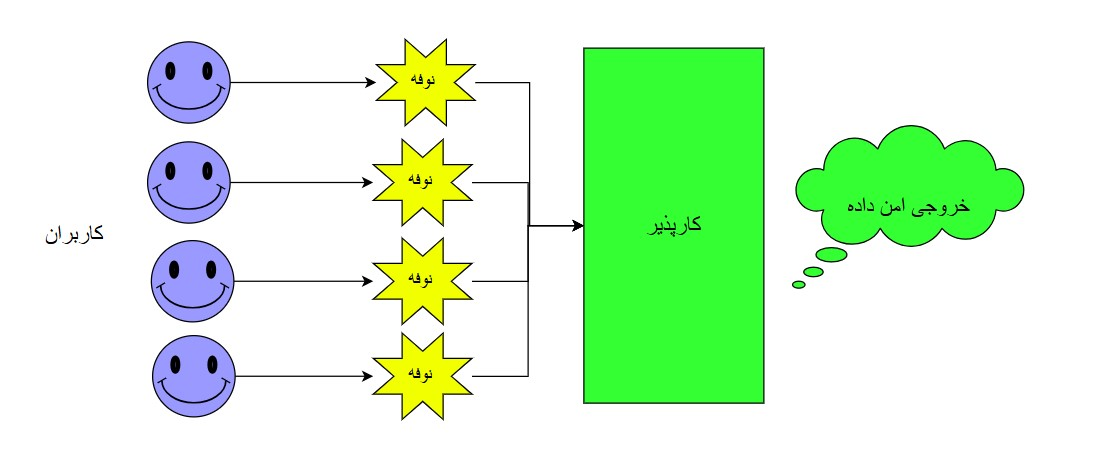
\includegraphics[width=0.9\textwidth]{figs/LDP.jpg}
  \caption{نحوه عملکرد حریم خصوصی تفاضلی محلی}
  \label{fig:LDP}
\end{figure}


\قسمت{حساسیت}

حساسیت\پانویس{Sensitivity} در زمینه حریم خصوصی داده‌ها به حداکثر تغییر در خروجی یک تابع به دلیل تغییر یک ورودی واحد اشاره دارد \مرجع{Dwork2011AFF}. به عبارت دیگر، حساسیت اندازه‌گیری می‌کند که چقدر می‌توان با تغییر یک ورودی، خروجی تابع را تحت تأثیر قرار داد. این ویژگی در طراحی سازوکار‌های حریم خصوصی تفاضلی محلی بسیار مهم است، زیرا تعیین می‌کند که چه مقدار نوفه باید به خروجی اضافه شود تا حریم خصوصی کاربران حفظ گردد.

\شروع{تعریف}[حساسیت]

حساسیت یک تابع $ f : \mathcal{X} \to \mathbb{R}^d$ به صورت زیر تعریف می‌شود:

\begin{equation}
\Delta f = \max_{x, x' \in \mathcal{X}} \|f(x) - f(x')\|
\end{equation}

\برچسب{تعریف: حساسیت}
\پایان{تعریف}


در عبارت بالا $\Delta f$ حساسیت تابع $f$ نامیده می‌شود و $\mathcal{X}$ دامنه ورودی ما است.

\قسمت{الگوریتم‌های حافظ حریم خصوصی تفاضلی}

\زیرقسمت{سازوکار لاپلاس}

سازوکار لاپلاس\پانویس{Laplace} در حریم خصوصی تفاضلی ایده‌ای ساده و در عین حال توانمند است. هرگاه بخواهیم آماری از داده‌ها مانند مجموع، میانگین و تعداد را منتشر کنیم، به‌جای پاسخ دقیق، همان پاسخ را با نوفه‌ای که از توزیع لاپلاس بدست می‌آید می‌فرستیم. مقدار پراکندگی این نوفه طوری تنظیم می‌شود که اگر اطلاعات یک فرد در پایگاه‌داده حذف یا اضافه شود، توزیع خروجی تقریباً تغییر نکند.  بدین‌ترتیب حضور یا عدم حضور آن فرد در نتیجه قابل تشخیص نیست. بزرگی نوفه به دو عامل بستگی دارد: حساسیت تابع و همچنین بودجهٔ حریم خصوصی. هرچه بودجه‌ی کمتری اختصاص دهیم حفاظت قوی‌تر شده و نوفه بیشتری اعمال می‌شود.

\شروع{تعریف}[سازوکار لاپلاس]

سازوکار لاپلاس روی یک تابع $ f : \mathcal{X} \to \mathbb{R}^d$ به صورت زیر تعریف می‌شود:

\begin{equation}
\mathcal{M}(D) = f(D) + \text{Lap}\left(\frac{\Delta f}{\epsilon}\right)
\end{equation}

\برچسب{تعریف: سازوکار لاپلاس}
\پایان{تعریف}

در عبارت بالا، ورودی مرکز یا $\mu$ در توزیع لاپلاس برابر صفر و همچنین ورودی مقیاس یا $b$ برابر $\frac{\Delta f}{\epsilon}$ در نظر گرفته شده است.


\زیرقسمت{سازوکار نمایی}

یکی از مشکلات سازوکار لاپلاس، عدم کارایی در مقادیر گسسته و غیر عددی است. از این رو سازوکار دیگری به نام سازوکار نمایی معرفی شد. این سازوکار چارچوبی فراهم می‌کند که در آن می‌توانیم تابع سودمنی دلخواه خود را تعریف کنیم. در واقع تابع $u$ هر ورودی و خروجی‌ تشکیل شده از پایگاه‌داده‌ی ما را به یک امتیاز سودمندی تبدیل می‌کند.

\begin{equation}
u : \mathbb{N}^{|X|} \times \mathcal{R} \rightarrow \mathbb{R}
\end{equation}

پس از محاسبه‌ی امتیاز هر خروجی، سازوکار گزینه‌ها را با احتمالی متناسب با توزیع نماییِ آن امتیاز انتخاب می‌کند. این انتخاب به‌گونه‌ای انجام می‌شود که گزینه‌های دارای امتیاز بالاتر، با احتمال بیشتری انتخاب شوند. این روش برای پرسش‌های غیرعددی (مثل «کدام محصول پرفروش‌تر است؟») بسیار سودمند خواهد بود. دقت کنید که ما اینجا نیاز به محاسبه حساسیت تابع سودمندی خود به شکل زیر داریم:

\begin{equation}
\Delta u = \max_{r \in \mathcal{R}} \max_{\substack{x,y \in \mathbb{N}^{|X|} \\ \|x - y\|_1 \leq 1}} |u(x,r) - u(y,r)|
\end{equation}

در نهایت سازوکار نمایی $\mathcal{M}_{E}(x,u,\mathcal{R})$ 
عنصر $r \in \mathcal{R}$ را با احتمالی متناسب با
$\exp\!\left(\frac{\varepsilon\,u(x,r)}{2\,\Delta u}\right)$
گزینش و اعلام می‌کند.

\زیرقسمت{پاسخ تصادفی}

پاسخ تصادفی روشی است که در نظرسنجی‌ها و جمع‌آوری داده‌های حساس کاربرد دارد. در این روش، به جای اینکه کاربر به‌طور مستقیم به یک سؤال پاسخ دهد، از یک سازوکار تصادفی استفاده می‌کند تا عدم قطعیت را به پاسخ خود اضافه کند. با اضافه کردن عدم قطعیت، مهاجم یا شخص متخاصم حتی اگر پاسخ نوفه‌دار شده‌ی کاربر را داشته‌باشد، نمی‌تواند با قطعیت جواب اصلی را مشخص کند. به بیان دیگر، کاربر با احتمال مشخصی پاسخ واقعی خود را ارائه می‌دهد و با احتمال دیگری پاسخ تصادفی دیگری را انتخاب می‌کند. این کار باعث می‌شود که احتمال شناسایی پاسخ واقعی کاربر کاهش یابد. مدل ریاضی پاسخ تصادفی توسط وارنر \مرجع{Warner1965RandomizedRA} معرفی شد.

\شروع{تعریف}[پاسخ تصادفی]

فرض کنید کاربر می‌خواهد به یک سؤال دودویی\پانویس{Binary} (بله/خیر) پاسخ دهد. اگر $x$ پاسخ واقعی کاربر باشد، سازوکار پاسخ تصادفی به صورت زیر عمل می‌کند:

\begin{equation}
\Pr[y = t] = 
\begin{cases} 
p, & \text{if} \quad t = x, \\[10pt]
1-p, & \text{if} \quad t \neq x
\end{cases}
\end{equation}

\برچسب{تعریف: پاسخ تصادفی}
\پایان{تعریف}

در عبارت بالا، $y$ پاسخ ارائه شده به سؤال است. $p$ احتمال اینکه کاربر پاسخ واقعی خود را ارائه دهد و $1{-}p$ احتمال این است که کاربر به طور تصادفی پاسخ مخالف را انتخاب کند. سازوکار پاسخ تصادفی اگر بخواهد $\epsilon{-}LDP$ باشد، باید مقدار $p$ را برابر $\frac{e^{\varepsilon}}{e^{\varepsilon}+1}$ قرار دهیم.

\زیرقسمت{پاسخ تصادفی عمومی}

پاسخ تصادفی به تنهایی جوابگوی مسائل پیچیده‌تر با دامنه بزرگتر نبود. پاسخ تصادفی عمومی\پانویس{Generalized Randomized Response}، شکل عمومی‌تر و انعطاف‌پذیرتر پاسخ تصادفی است \مرجع{Kairouz2016DiscreteDE, Kairouz2014ExtremalMF}. این الگوریتم را به اختصار، «جی آر آر» می‌نامند.

\شروع{تعریف}[پاسخ تصادفی عمومی]

فرض کنید کاربر می‌خواهد به یک سؤال با $k$ گزینه پاسخ دهد. اگر $x$ پاسخ واقعی کاربر باشد، سازوکار پاسخ تصادفی عمومی به صورت زیر عمل می‌کند:

\begin{equation}
\Pr[y = t] = 
\begin{cases} 
p, & \text{if} \quad t = x, \\[10pt]
\frac{1 - p}{k - 1}, & \text{if} \quad t \neq x
\end{cases}
\label{equ:GRR}
\end{equation}

\برچسب{تعریف: پاسخ تصادفی عمومی}
\پایان{تعریف}

سازوکار پاسخ تصادفی اگر بخواهد $\epsilon{-}LDP$ باشد، باید مقدار $p$ را برابر $\frac{e^{\varepsilon}}{e^{\varepsilon}+k-1}$ قرار دهیم.

پژوهش آرکولزی و همکاران \مرجع{Arcolezi2023RevealingTT} یک چارچوب نرم‌افزاری را برای حسابرسی و ارزیابی عملی پروتکل‌های حریم خصوصی تفاضلی محلی معرفی می‌کند. در نتیجه آزمایشات این پژوهش، پاسخ تصادفی عمومی بهترین عملکرد را داشته است. به بیان دیگر اتلاف حریم خصوصی که به صورت عملی برای پاسخ تصادفی عمومی اندازه‌گیری شد، بسیار نزدیک به تضمین نظری آن بوده است. یعنی این سازوکار دقیقاً همان سطحی از حریم خصوصی را که ادعا می‌کند، در عمل نیز ارائه می‌دهد و بیش از حد محافظه‌کارانه عمل نمی‌کند. دلیل این امر، سادگی آن و عدم وجود مراحل کدگذاری پیچیده است که باعث از دست رفتن اطلاعات نمی‌شود.

\زیرقسمت{الگوریتم تصادفی‌سازی متقارن}

به الگوریتم‌هایی که در فرآیند تصادفی‌سازی برای حفظ حریم خصوصی کاربران، احتمال حفظ مقدار اصلی داده‌ها برابر با احتمال تغییر آن‌ها باشد، متقارن می‌گوییم. به عنوان مثال در مسائلی که ورودی با دامنه دودویی دارند، احتمال زیر برقرار است:

\begin{equation}
Pr[y = 1 | x = 1] = Pr[y = 0 | x = 0] 
\end{equation}

در عبارت بالا، $x$ ورودی و $y$ خروجی الگوریتم است.

\قسمت{ترکیب متوالی}

در زمینه حریم خصوصی، ترکیب متوالی\پانویس{Sequential Composition} به این صورت تعریف می‌شود که اگر شما چندین سازوکار تصادفی را به‌طور متوالی روی یک مجموعه داده اجرا کنید، حریم خصوصی شما به‌طور کلی نقض می‌شود. حتی اگر هر یک از این سازوکار‌ها جداگانه ایمن باشند، در نهایت نمی‌توانید حریم خصوصی را تضمین کنید \مرجع{nissim2012approximately}. این اصل ساده اما سرنوشت‌ساز، طراحان الگوریتم‌های حریم خصوصی را مجبور می‌کند بودجهٔ حریم خصوصی را میان سازوکارهای مختلف تقسیم کنند. از آنجایی که بوجه‌ی حریم خصوصی محدود است، اگر تعداد سازوکارهای مختلف زیاد باشد، بودجه‌ی کمی به هر کدام می‌رسد و به سبب آن سودمندی الگوریتم کاهش میابد.

به بیان ریاضی، پس از اجرای $k$ سازوکار مستقل روی یک مجموعه داده که هرکدام $\epsilon{-}LDP$ هستند، می‌توان گفت الگوریتم کلی ما با بودجه‌ای برابر با مجموع تمام بودجه‌ها، حریم خصوصی تفاضلی را ارضا می‌کند:

$$\mathcal{M}_i(x) \quad satisfies \quad \epsilon_i{-}LDP$$
$$\mathcal{M} = \{ \mathcal{M}_1 , \mathcal{M}_2 , ... , \mathcal{M}_m \} \quad satisfies \quad \sum_{i=1}^{m} \epsilon_i{-}LDP$$

در سامانه‌هایی که پرس‌و‌جو‌های\پانویس{Query} متعدد روی یک معیار داریم (مانند دریافت میزان مصرف باتری هر یک ساعت یکبار)، هر بار باید روی یک داده نوفه اعمال کنیم و به سمت کارپذیر بفرستیم. گرچه مقدار خام داده ممکن است هر بار تغییر کند، ولی چون از یک جنس است و مربوط به یک معیار می‌شود، قانون ترکیب متوالی روی آن صدق می‌کند. بودجه‌ی حریم خصوصی بین تعداد استفاده از سازوکار تصادفی‌سازی تقسیم شده و سودمندی کاهش میابد.

شایان ذکر است که در داده‌های با ابعاد بالا نیز، با چالش ترکیب متوالی روبه‌رو هستیم. در داده‌های با ابعاد بالا، احتمال وجود وابستگی میان ابعاد زیاد می‌شود (مانند ارتباط مستقیم بین سن و میزان درآمد). زمانیکه سازوکارهای تصادفی‌سازی را روی ابعاد وابسته به هم اعمال می‌کنیم، مانند این است که به یک مجموعه داده نوفه تزریق می‌کنیم. از این رو شامل قانون ترکیب متوالی شده و بوجه‌ی حریم خصوصی بین سازوکارها تقسیم می‌شود.

\قسمت{ترکیب موازی}

در ترکیب موازی\پانویس{Parallel Composition}، الگوریتم‌های مختلف حریم خصوصی تفاضلی به طور همزمان روی یک یا چند پایگاه‌داده مجزا  از یکدیگر اعمال می‌شوند \مرجع{mcsherry2009privacy}. در این حالت، بودجه‌ی الگوریتم کلی برابر با حداکثر بودجه‌ی الگوریتم‌هاست:

$$\mathcal{M}_i(x) \quad satisfies \quad \epsilon_i{-}LDP$$
$$ \mathcal{M} = \{ \mathcal{M}_1 , \mathcal{M}_2 , ... , \mathcal{M}_m \} \quad satisfies \quad \max \{ \epsilon_1 , \epsilon_2 , ... , \epsilon_m \}{-}LDP$$

\قسمت{روش‌های کدگذاری}

هر کاربر به منظور ارسال داده‌ها سمت کارپذیر، باید ابتدا اطلاعات خود را در فرمت خاصی کدگذاری\پانویس{Encode} کند. اینکار به دو دلیل نیاز است:

\شروع{شمارش}
\فقره افزایش سرعت ارسال پیام
\فقره بهبود فرایند تصادفی‌سازی
\پایان{شمارش}

\زیرقسمت{کدگذاری مستفیم}

کدگذاری مستقیم\پانویس{Direct Encoding} یکی از روش‌های ساده برای کدگذاری مقادیر ورودی در پروتکل‌های حفاظت از حریم خصوصی محلی است. در این روش، داده‌ی هر کاربر بدون هیچ‌گونه تبدیل اولیه مستقیماً به عنوان خروجی کدگذاری‌شده و ارسال می‌شود. این روش برای مواردی که دامنه داده‌ها کوچک است (مانند داده‌های طبقه‌بندی‌شده یا مقادیر گسسته محدود) مناسب‌تر خواهد بود. این کدگذاری در پژوهش \مرجع{Wang2016PrivateWH} استفاده شده است.

\begin{equation}
 v = Encode(v)
\end{equation}

برای تصادفی‌سازی در این کدگذاری، باید از سازوکار تصادفی‌سازی عمومی استفاده کرد. دقت کنید که کارایی و عملکرد این روش با افزایش دامنه، به شدت کاهش میابد. از آنجایی که در الگوریتم تصادفی‌سازی عمومی، مقدار $p$ برابر $\frac{e^{\varepsilon}}{e^{\varepsilon}+k-1}$ است، با افزایش دامنه یا همان $k$، احتمال انتخاب شدن مقدار اصلی در تصادفی‌سازی کاهش یافته و به سبب آن، سودمندی دلخواه بدست نمی‌آید. همچنین یکی دیگر از معایب این روش، هزینه‌ی ارتباطی\پانویس{Communication Cost} بالا است.

\زیرقسمت{کدگذاری یکانی}

کدگذاری یکانی\پانویس{Unary Encoding} یکی از روش‌های متداول برای کدگذاری مقادیر ورودی در پروتکل‌های حفاظت از حریم خصوصی تفاضلی محلی است. در این روش، هر مقدار ورودی به یک بردار دودویی با طول ثابت تبدیل می‌شود. تنها یک بیت از این بردار که نماینده ورودی است، مقدار 1 دارد و بقیه بیت‌ها 0 هستند.

\begin{equation}
Encode(v) = [0, \text{···} ,0,1,0, \text{···} , 0], \quad \text{\lr{only the v-th position is 1}}
\end{equation}

به منظور تصادفی‌سازی از فرمول زیر استفاده می‌کنیم. $p$ احتمال 1 شدن بیتی است که قبلا مقدار 1 داشته است. همچنین $q$ احتمال 1 شدن بیتی است که قبلا مقدار 0 داشته است:

\begin{equation}
\Pr[y = 1] =
\begin{cases} 
p, & \text{if} \quad x = 1, \\[10pt]
q, & \text{if} \quad x = 0.
\end{cases}
\end{equation}

اگر شرط زیر برقرار باشد، می‌توان گفت پروتکل کدگذاری یکانی، حریم خصوصی تفاضلی را ارضا کرده است:


\begin{equation}
\epsilon = \ln \left( \frac{p(1 - q)}{(1 - p)q} \right)
\label{equ:unary}
\end{equation}

\زیرقسمت{کدگذاری یکانی متقارن}

پروتکل کدگذاری یکانی متقارن\پانویس{Symmetric Unary Encoding} به این صورت تعریف می‌شود که حاصل جمع مقادیر احتمال $p$ و $q$ برابر 1 باشد:
$$p + q = 1$$
با توجه به قاعده \رجوع{equ:unary}، مقادیر $p$ و $q$ به صورت زیر بدست می‌آیند:

$$p = \frac{e^{\epsilon/2}}{e^{\epsilon/2} + 1}, \quad q = \frac{1}{e^{\epsilon/2} + 1}$$

\زیرقسمت{درهم‌سازی محلی}

در پروتکل کدگذاری یکانی، هزینه‌ی ارتباطی به صورت خطی با زیاد شدن دامنه‌ی ورودی، افزایش میابد. این افزایش هزینه در بعضی برنامه‌های کاربردی موجب بروز تاخیر بسیار زیاد در عملکرد سامانه می‌شود. بنابراین به پروتکل دیگری نیاز داریم که بزرگ شدن دامنه‌ی ورودی، تاثیر چندانی در هزینه ارتباطی نداشته باشد.

ایده‌ی اولیه این است که از یک تابع درهم‌ساز\پانویس{Hash Function} استفاده کرده و اندازه‌ دامنه‌ی ورودی را کاهش دهیم. این ایده مشکل تصادم\پانویس{Collision} را به همراه دارد. به بیان دیگر، دو ورودی به یک خروجی تبدیل شده و در زمان کدگشایی\پانویس{Decode} نمی‌توان مقدار درست ورودی را بدست آورد. در پژوهش رپور \مرجع{erlingsson2014rappor} چندین راه برای حل این مشکل ارائه شده است:

\شروع{شمارش}
\فقره استفاده از چند تابع درهم‌ساز به منظور کاهش احتمال تصادم
\فقره استفاده از مفهوم گروه\پانویس{Cohort} که در آن هر گروه دارای مجموعه‌ای از توابع درهم‌ساز خواهد بود.
\پایان{شمارش}

البته با توجه به روش‌های مذکور، نمی‌توان به صورت قطعی مشکل تصادم را حل کرد و این مشکل در کاهش سودمندی تأثیر می‌گذارد. روش بهتر این است که هر کاربر توابع درهم‌ساز محلی خود را داشته باشد. به این روش، درهم‌ساز محلی\پانویس{Local Hashing} می‌گوییم. این روش به صورت کارا در الگوریتم‌های حفظ حریم خصوصی تفاضلی محلی استفاده می‌شود. کاربران با کمک توابع درهم‌ساز، ابتدا دامنه‌ی داده‌های خود را کاهش داده، تصادفی‌سازی کرده و در نهایت به سمت کارپذیر ارسال می‌کنند. در ادامه تعریف درهم‌ساز محلی دودویی را ارائه می‌دهیم:

\شروع{تعریف}[درهم‌ساز محلی دودویی]

فرض کنید $\mathbb{H}$ یک خانواده جهانی از توابع درهم‌ساز باشد. هر تابع درهم‌ساز $H \in \mathbb{H}$، یک ورودی با دامنه‌ی $d$ را به یک عدد تک بیتی تبدیل می‌کند. شرطی روی این خانواده از توابع درهم‌ساز اعمال می‌شود به صورت زیر خواهد بود:

\begin{equation}
\forall x, y \in [d], x \neq y : \Pr_{H \in \mathbb{H}} [H(x) = H(y)] \leq \frac{1}{2}
\end{equation}

\برچسب{تعریف: درهم‌ساز محلی دودویی}
\پایان{تعریف}

به منظور تصادفی‌سازی از فرمول زیر استفاده می‌کنیم:

$$\text{Perturb}_{\text{BLH}}(\langle H, b \rangle) = \langle H, b' \rangle, \quad \Pr[b' = 1] = 
\begin{cases} 
p = \dfrac{e^\epsilon}{e^{\epsilon}+1}, & \text{if} \quad b = 1 \\ 
q = \dfrac{1}{e^{\epsilon}+1}, & \text{if} \quad b = 0 
\end{cases}$$

\زیرقسمت{بلوم فیلتر}

بلوم‌فیلتر\پانویس{Bloom Filter} یک ساختار داده‌ای است که هدف اصلی آن انجام عملیات بررسی عضویت (یعنی تعیین اینکه یک عنصر در مجموعه‌ای وجود دارد یا خیر) با استفاده حداقلی از حافظه است. این فیلتر به ما کمک می‌کند تا سریعاً امکان وجود یک عنصر را بدون نیاز به ذخیره کل مجموعه در حافظه تشخیص دهیم.

فرض کنید آرایه‌ای از بیت‌ها (معمولاً همه صفر) و چند تابع درهم‌ساز داریم. مطابق شکل \رجوع{fig:BloomFilter} زمان درج هر عنصرِ جدید، آن را با همه توابع درهم‌سازی کرده و مقدار 1 برای بیت‌های متناظر درنظر گرفته می‌شود. دقت کنید که ممکن است درهم‌سازی توابع، تصادم داشته باشد و چند بیت 1 روی هم بیفتند. هنگام پرس‌وجوی عنصر،  دوباره باید با همه‌ی توابع درهم‌سازی شود و اگر همه‌ی بیت‌های متناظر یک باشند، می‌گوییم این عنصر احتمالاً در آرایه وجود دارد. حتی اگر یکی صفر باشد قطعاً عنصر مورد نظر در آرایه وجود ندارد. با تنظیم اندازهٔ آرایه و تعداد توابع هش، می‌توان احتمال خطا را به دلخواه کم کرد. از همین ویژگی در پژوهش رپور نیز بهره گرفته شده تا رشته‌های دلخواه کاربران به‌صورت فشرده و بی‌نیاز از فهرست پیش‌تعریف‌شده گزارش شود و حریم خصوصی حفظ گردد.

بلوم فیلتر در بسیاری از سیستم‌ها و سرویس‌ها استفاده می‌شود از جمله:

\شروع{فقرات}
\فقره گوگل کروم: برای ویژگی مرور امن\پانویس{Safe Browsing} از بلوم فیلتر استفاده می‌شود تا به سرعت خطرناک بودن آدرس‌های اینترنتی را بررسی کند.
\فقره مدیُم\پانویس{Medium}: از بلوم فیلتر برای جلوگیری از نمایش پست‌هایی که کاربر قبلاً دیده است، استفاده می‌کند.
\فقره کساندرا\پانویس{Cassandra} و اچ بیس\پانویس{HBase}: برای بهینه‌سازی جستجوی داده‌ها در جدول‌های ذخیره‌شده در دیسک استفاده می‌شود.
\فقره آکامای\پانویس{Akamai}: در سرویس‌های حافظه نهان\پانویس{Cache} خود برای بهبود سرعت و کارایی تحویل محتوا از بلوم فیلتر استفاده می‌کند.
\پایان{فقرات}

\begin{figure}[h]
  \centering
  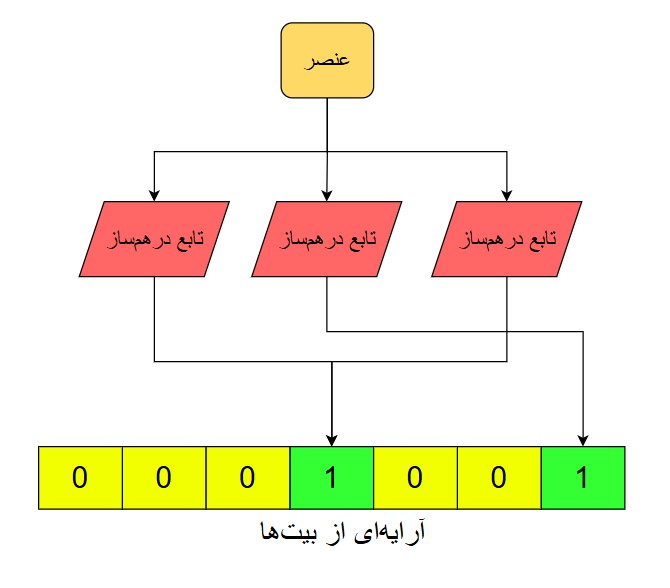
\includegraphics[width=0.9\textwidth]{figs/BloomFilter.jpg}
  \caption{شیوه‌ی درج عنصر با استفاده از بلوم فیلتر}
  \label{fig:BloomFilter}
\end{figure}




\فصل{کارهای پیشین}

در این فصل به بررسی کارها و پژوهش‌های پیشین در دو حوزه داده‌های ابعاد بالا و داده‌های در حال تغییر می‌پردازیم. ابتدا چالش‌های هر کدام را بررسی کرده و راه‌حل‌های موجود را بیان می‌کنیم. همچنین مزایا و معایب هر کدام ارائه می‌شود تا مناسب‌ترین راه‌حل مشخص شود.

\قسمت{داده‌های با ابعاد بالا}

هنگام جمع‌آوری داده‌های چندبُعدی با حفظ حریم خصوصی تفاضلی، کارپذیر ابتدا داده‌ی نوفه‌دار شده‌ی هر شخص یا برنامه کاربردی را دریافت کرده و سپس شروع به تحلیل آماری روی هر بعد می‌کند. در اغلب شیوه‌های رایجِ جمع‌آوری داده‌های چندبُعدی، برای صیانت از حریم خصوصی کاربران، هر ویژگی را جداگانه نوفه‌دار می‌کنند. با توجه به قانون ترکیب متوالی ناچارا بودجه‌ی محدود حریم خصوصی میان همهٔ ابعاد پخش می‌شود. کاهش بودجه موجب تزریق نوفه بیش از اندازه شده و در نتیجه سودمندی به شکل چشمگیری کاهش میابد.

به بیان دیگر در داده‌های با ابعاد بالا، چالش اصلی به همبستگی‌های احتمالی بین ابعاد مختلف بازمی‌گردد. این همبستگی‌ها باعث می‌شود تغییر در یک بعد به تغییرات در ابعاد دیگر منجر شود و حساسیت کل سیستم افزایش یابد. در اکثر الگوریتم‌های حافظ حریم خصوصی تفاضلی، افزایش حساسیت موجب اضافه‌شدن بیش از انداره‌ی نوفه به داده‌ها خواهد شد. بنابراین، یافتن رویکردهایی که بتوانند حساسیت را کاهش دهند یا از روش‌های هوشمندانه‌تر برای تخصیص نوفه استفاده کنند، ضروری است. 

برای نمونه، سازوکار کلاسیک لاپلاس \مرجع{dwork2006calibrating}، نوفه در توزیع لاپلاس را به صورت تصادفی روی تک‌تک بُعدها اعمال می‌کند. در این روش، مقدار نوفه به‌شکلی بیش‌ازخطی با تعداد ابعاد رشد می‌کند و بدین ترتیب سودمندی داده‌های چندبُعدی به‌شدّت افت خواهد کرد. در ادامه با راه‌حل‌های این چالش بیشتر آشنا می‌شویم.

\زیرقسمت{نمونه‌برداری}

معمولا مقالاتی که روی داده‌های با ابعاد بالا کار می‌کنند، از نمونه‌برداری استفاده می‌کنند. در واقع سعی می‌کنند بخشی از داده را به عنوان نماینده‌ی تمام داده‌ها در نظر گرفته و فقط برای آن بخش الگوریتم‌های حفظ حریم خصوصی تفاضلی اعمال شود. با این کار، تنها به بخشی از داده‌ها، نوفه تزریق می‌شود. البته یکی از مشکلات نمونه‌برداری این است که نیازمند تعداد بسیار زیادی کاربر خواهد بود تا بتوان اطلاعات آماری مفیدی از کل داده‌ها به دست آورد.

\زیرزیرقسمت{پژوهش دوچی و همکاران}

سازوکار تکه‌ای\پانویس{Piecewise} که توسط دوچی ارائه شده است \مرجع{Duchi2016MinimaxOP}، برای حل مشکل تقسیم بودجهٔ حریم خصوصی، سراغ نمونه‌گیری از داده می‌رود. در این پژوهش داده‌ها به صورت بردار و مختصات درنظر گرفته می‌شوند. در واقع هر رکورد (مثلاً یک کاربر، یک حسگر، یا یک آزمایش) داراری مجموعه‌ای از ویژگی‌ها است و می‌توانیم این ویژگی‌ها را مانند محورهای یک فضای چندبعدی تصور کنیم. فرض کنید سه ویژگی «سن»، «قد» و «درآمد» داریم؛ آن‌گاه هر فرد نقطه‌ای در فضای سه‌بعدی است که مختصاتش به‌ترتیب عدد سن، قد و درآمد اوست. برای نمونه اگر ۱۰۰ خصوصیت زیستی یا آماری داشته باشیم، همان نقطه اکنون در فضایی ۱۰۰‌بعدی قرار می‌گیرد و برداری با ۱۰۰ عدد پی‌درپی تشکیل می‌دهد. بنابراین «بردار» صرفاً لیستی منظم از مقادیر است و «مختصات» خانه‌های این لیست‌اند که به هر ویژگی برچسب می‌زنند. 

سازوکار تکه‌ای برای آن‌که بتواند تحلیل‌های آماری روی بردارهای با ابعاد بالا را با حفظ حریم خصوصی محلی انجام دهد، به‌جای افزودن نوفه مستقل به تک‌تک مختصات (کاری که در ابعاد زیاد دقّت را نابود می‌کند)، نوفه به بردارهای «خلاصه» شده وارد می‌شود. به صورت خلاصه، در یک عملیات پیچیده، کاربر با پرتاب سکه، یک نوفه‌ی خاص را روی جهت بردار اعمال می‌کند. به بیان دیگر نوفه فقط به مختصات مؤثر، تزریق می‌شود و اندازه‌ی بردار دستکاری نمی‌گردد.

چندین پژوهش تلاش کردند تا از ویژگی‌های همبسته نمونه برداری کنند. با این کار، بودجه‌ی حریم خصوصی را به شکل هوشمندانه بین ابعاد داده پخش می‌کنند. به منظور یافتن ویژگی‌های همبسته، معمولا از دو مفهوم آماری \مهم{اطلاعات متقابل} و \مهم{بی‌نظمی} استفاده می‌شود. 

اطلاعات متقابل معیاری ست که میزان اطلاعاتی را که یک متغیر تصادفی در مورد متغیر دیگر به ما می‌دهد، اندازه‌گیری می‌کند. یعنی اگر یکی را بدانیم، عدم قطعیتِ ما درباره‌ی دیگری تا چه حد کم می‌شود. هرچه مقدار این معیار بیشتر باشد، وابستگی یا هم‌بستگی میان آن دو متغیّر قوی‌تر است.

\شروع{تعریف}[اطلاعات متقابل]

از دید ریاضی، برای دو متغیّر تصادفی گسسته‌ی $X$ و $Y$ با توزیع مشترک $p(x,y)$ و توزیع‌های حاشیه‌ای $p(x)$ و $p(y)$، اطلاعات متقابل چنین تعریف می‌شود:

\begin{equation}
I(X;Y) = \sum_{x} \sum_{y} \hat{P}(x, y) \log \frac{\hat{P}(x, y)}{\hat{P}(x) \hat{P}(y)}
\label{equ:mutual}
\end{equation}

\برچسب{تعریف: اطلاعات متقابل}
\پایان{تعریف}

بی‌نظمی\پانویس{Entropy}، که در فیزیک و نظریه‌ی اطلاعات به نام «آنتروپی» شناخته می‌شود، معیاری برای سنجش پراکندگی حالت‌های یک سامانه است. هرچه تعداد حالت‌های ممکنِ سازگار با مشاهدهٔ ما بیش‌تر باشد، پیش‌بینی رفتار آینده‌ی سامانه دشوارتر و «بی‌نظمی» آن بالاتر است؛ برعکس، در سامانه‌های منظم، گزینه‌های کمتری برای چگونگی چیدمان اجزا وجود دارد و قطعیت بیش‌تری داریم. به زبان ساده، آنتروپی اندازه‌ای از بی‌خبری یا عدم قطعیت ما درباره‌ی وضعیت دقیق اجزاست.

\زیرزیرقسمت{پژوهش چن و همکاران}

پژوهش چن و همکاران \مرجع{chen2023locally} روشی به نام سم‌پرایو‌سین ارائه می‌دهد که براساس اطلاعات متقابل\پانویس{Mutual Information}، ارتباط میان ویژگی‌ها را بدست آورده و تنها از جفت ویژگی‌هایی که بیشترین ارتباط را دارند، نمونه‌برداری می‌کند. این پژوهش به‌جای ارسالِ کلِ رکورد و نوفه‌دار کردن همه‌ی ابعاد، تنها یک جفت ویژگی از هر کاربر را انتخاب و پس از نوفه‌دار کردن همان دو مقدار، به کارپذیر می‌فرستد. انتخاب این جفت ویژگی تصادفی نیست؛ احتمال برگزیده‌شدن هر زوج، متناسب با اطلاعات متقابل به‌روز‌شده‌ی آن‌ها است. زوج‌هایی که بیش‌ترین هم‌بستگی را دارند، با احتمال بیشتری انتخاب شده و ساختار واقعیِ داده تا حد ممکن حفظ می‌شود. سپس هر یک از دو مقدار انتخاب‌شده با بودجهٔ $\epsilon / 2$ نوفه‌دار می‌شود. بدین ترتیب کل فرایند همچنان $\epsilon {-}LDP$ باقی می‌ماند، در حالی که حجم ارتباطی و نوفه تزریق‌شده فقط به همان دو بُعد محدود می‌شود. در ادامه، این داده‌های نمونه‌برداری‌شده برای بازسازی مجموعه داده‌های مصنوعی به کار می‌روند و همچنان ارتباط میان ویژگی‌ها حفظ می‌شود.

\زیرزیرقسمت{پژوهش وانگ و همکاران}

پژوهشی که توسط وانگ و همکاران \مرجع{Wang2019CollectingAA} انجام شده است، یک الگوریتم حافظ حریم خصوصی تفاضلی برای جمع‌آوری داده‌های عددی ارائه می‌دهد. سپس الگوریتم خود را برای داده‌های چند بُعدی گسترش می‌دهد. این پژوهش ابتدا توضیح می‌دهد که واریانس\پانویس{Variance} کمتر در الگوریتم‌های حریم خصوصی به معنای دقت بیشتر در میانگین نتایج است. سازوکار تکه‌ای \مرجع{Duchi2016MinimaxOP} واریانس بالایی داشته و دقت نتایج پایین است. برای داده‌های چندبعدی، نویسندگان به دو مشکل اصلی سازوکار تکه‌ای اشاره می‌کنند. اول اینکه این الگوریتم پیچیدگی بالایی دارد و دوم اینکه تنها برای مقادیر عددی قابل استفاده است.
به همین دلیل، نویسندگان دو الگوریتم جدید به نام‌های پی‌-ام و اچ‌-ام معرفی می‌کنند که با کاهش واریانس، نتایج دقیق‌تری ارائه می‌دهند. \مهم{سازوکار پی-ام} برای هر عدد در بازه‌ی ‎$[{-}1, 1]‎$ سه ناحیه تعریف می‌کند: یک قطعه‌ی مرکزی و دو قطعه‌ی کناری‌ در چپ و راست. ابتدا با یک پرتاب تصادفی تصمیم می‌گیرد در کدام ناحیه نمونه بردارد. احتمال افتادن در قطعهٔ مرکزی عمداً بیشتر است تا خروجی غالباً به مقدار حقیقی نزدیک بماند، ولی اگر به قطعات کناری برود فاصله‌ی بیشتری با مقدار اصلی پیدا می‌کند. این فاصله همان نوفه‌ای است که باعث حفظ حریم خصوصی تفاضلی می‌شود. به این ترتیب داده همچنان در بازه‌ای محدود باقی می‌مانند و با کوچک‌تر شدن مقدار نوفه، واریانس نیز پایین می‌آید، در نتیجه دقّت حفظ می‌شود.

\مهم{سازوکار اِچ-اِم} ترکیبی هوشمندانه از پی-اِم و تکه‌ای است. هر بار که می‌خواهد داده را نوفه‌دار کند، سکه‌ای پرتاب می‌شود که با احتمال $\alpha$ شیر می‌آید. اگر شیر آمد، پی-اِم اجرا می‌شود؛ اگر خط آمد، همان روش تکه‌ای به کار می‌رود. مقدار $\alpha$ به‌طور تحلیلی طوری انتخاب می‌شود که کل واریانس نوفه را در بدترین حالت کمینه کند. با توجه به پی-ام ،برای $\epsilon$ بزرگ $\alpha$ تقریباً یک است، و  با توجه به روش تکه‌ای، برای $\epsilon$ خیلی کوچک $\alpha$ به صفر میل خواهد کرد. بنابراین اِچ-اِم در همهٔ شرایط از هر دو رقیب یا بهتر است یا دست‌کم بدتر نمی‌شود.

برای رفع مشکل داده‌های با ابعاد بالا، پژوهش یک الگوریتم جدید پیشنهاد می‌دهد. این الگوریتم بیان می‌کند که نیازی نیست همه ابعاد داده نوفه‌دار شوند. کافیست تنها به ابعاد محدودی که به صورت تصادفی انتخاب می‌شوند، نوفه اضافه کرد. اگر $k$ بُعد را انتخاب کنیم، باید بودجه‌ی حریم خصوصی $\epsilon / k$ را به هر بُعد اختصاص دهیم. چون $k$ معمولاً خیلی کوچک‌تر از تعداد کل ابعاد است، هر ویژگی سهم بودجه‌ی بزرگ‌تری می‌گیرد و نوفه‌ی کمتری به آن تزریق می‌شود. در نتیجه سامانه می‌تواند روی داده‌های با ابعاد بالا تحلیل‌های آماری مثل میانگین یا حتی گرادیان‌های یادگیری ماشین را با خطای کمی برآورد کند.

\زیرزیرقسمت{پژوهش آرکولزی و همکاران}

پژوهش \مرجع{Arcolezi2021ImprovingTU} نیز از نمونه‌برداری در الگوریتم خود استفاده کرده‌است. این مقاله یک راهکار جدید برای چالش جمع‌آوری داده‌های چندبُعدی و در حال تغییر تحت محدودیت‌های حریم خصوصی تفاضلی محلی ارائه می‌دهد. مشکل اصلی این است که وقتی چندین ویژگی از یک کاربر در بازه‌های زمانی مختلف جمع‌آوری می‌شود، حفظ حریم خصوصی به شدت دشوار شده و  سودمندی کاهش می‌یابد. این پژوهش با بهبود پروتکل‌های موجود و ارائه یک الگوریتم جدید به نام الومفری\پانویس{ALLOMFREE}، راهکار جامعی برای تخمین شمارش داده‌ها فراهم می‌کند.

راهکار این پژوهش برای مدیریت داده‌های با ابعاد بالا، بر یک ایده هوشمندانه استوار است. به جای اینکه هر کاربر بخشی از بودجه حریم خصوصی خود را به هر یک از ویژگی‌هایش اختصاص دهد، به صورت تصادفی تنها یک ویژگی را انتخاب کرده و تمام بودجه حریم خصوصی را به همان یک ویژگی اختصاص می‌دهد. روش الومفری برای حفظ کارایی به صورت تطبیقی و هوشمندانه عمل می‌کند. پس از اینکه کاربر یک ویژگی را به صورت تصادفی انتخاب کرد، روش الموفری بر اساس مشخصات آن ویژگی (به‌ویژه تعداد مقادیر ممکن برای آن) و پارامترهای حریم خصوصی، محاسبه می‌کند که کدام پروتکل از بین پاسخ تصادفی عمومی و کدگذاری یکانی متقارن خطای کمتری خواهد داشت.

در واقع پروتکلی که واریانس کمتری تولید می‌کند، برای ارسال داده انتخاب می‌شود. به عبارت دیگر، الومفری به‌جای استفاده از یک راه‌حل ثابت، بهترین ابزار را برای هر موقعیت خاص انتخاب می‌کند و در نتیجه دقت تخمین شمارش به شدت بهبود می‌یابد. این پژوهش علاوه بر فعالیت در زمینه‌ی داده‌های با ابعاد بالا، در خصوص داده‌های در حال تغییر نیز راه‌حل‌هایی ارائه می‌کند که در بخش‌های بعدی توضیح می‌دهیم.

\زیرزیرقسمت{پژوهش رحمان صیام و همکاران}

پژوهش رحمان صیام و همکاران \مرجع{Seeam2025FrequencyEO} یک راهکار نوآورانه به نام «پاسخ تصادفی همبسته» برای جمع‌آوری و تحلیل داده‌های چند بُعدی با حفظ حریم خصوصی تفاضلی محلی ارائه می‌دهد. این پژوهش برای غلبه بر مشکلات داده‌های با ابعاد بالا، یک رویکرد هوشمندانه را معرفی می‌کند که از همبستگی بین داده‌ها به نفع خود استفاده می‌کند. رویکرد معرفی شده شامل مراحل زیر است:

\شروع{فقرات}

\فقره یادگیری همبستگی‌ها به صورت خصوصی: در این مرحله، گروه کوچکی از کاربران تمام داده‌های خود را با استفاده از یک روش معمول حریم خصوصی تفاضلی محلی (که نوفه‌ی زیادی دارد) ارسال می‌کنند. هدف این است که کارپذیر مرکزی بتواند الگوها و روابط آماری (همبستگی) بین خصوصیات مختلف را به صورت کاملاً خصوصی و بدون دیدن داده‌های واقعی، تخمین بزند.

\فقره جمع‌آوری داده مبتنی بر همبستگی: اکنون هر کاربر به جای ارسال تمام اطلاعات، به صورت تصادفی فقط یکی از خصوصیات خود را انتخاب می‌کند. سپس تمام بودجه حریم خصوصی را فقط روی همان یک خصوصیت متمرکز کرده و آن را ارسال می‌کند. سایر خصوصیات فرد، به جای ارسال مستقیم، بر اساس همبستگی‌های یادگرفته شده در مرحله اول و مقدار ارسال‌شده‌ی همان یک خصوصیت، به صورت مصنوعی و احتمالی بازسازی می‌شوند.

\پایان{فقرات}

\زیرزیرقسمت{پژوهش یوان و همکاران}

پژوهش یوان و همکاران \مرجع{Yuan2025LocalDP} مانند پژوهش‌های پیشین راهکاری مبتنی بر نمونه‌برداری برای حفظ حریم خصوصی داده‌های چندبُعدی در سیستم‌های محاسباتی توزیع‌شده ارائه می‌دهد. راهکار پیشنهادی به جای اینکه به تمام اجزای داده نوفه اضافه کند، برای هر جزء از داده یک تصمیم احتمالی می‌گیرد:

\شروع{فقرات}

\فقره با احتمال بالا (مثلاً ۹۹٪)، مقدار اصلی داده را دست‌نخورده و بدون تغییر باقی می‌گذارد.

\فقره با احتمال پایین (مثلاً ۱٪)، به آن مقدار، نوفه کنترل‌شده (از نوع گوسی یا لاپلاس) اضافه می‌کند.

\پایان{فقرات}

این رویکرد باعث می‌شود که مجموع نوفه تزریق‌شده به کل داده به مراتب کمتر از روش‌های سنتی باشد. علاوه بر این، پژوهشگران نسخه‌ای پیشرفته‌تر از الگوریتم خود را نیز معرفی می‌کنند که در آن می‌توان با استفاده از یک «ماتریس وزن»، بخش‌های مهم‌تر یا حساس‌تر داده (مانند چهره افراد در یک تصویر) را شناسایی کرد و سطح بالاتری از حفاظت را برای آن‌ها اعمال نمود؛ در حالی که به بخش‌های کم‌اهمیت‌تر (مانند پس‌زمینه تصویر) نوفه‌ی کمتری اضافه می‌شود.


\زیرقسمت{خوشه‌بندی}

یک راه‌حل اساسی برای اختصاص هدفمند بودجه‌ی حریم خصوصی به ابعاد داده، خوشه‌بندی\پانویس{Clustering} است. معمولا ابعاد همبسته در یک دسته قرار می‌گیرند. با توجه به اینکه درون هر دسته چند ویژگی قرار می‌گیرد، می‌توان بودجه‌ی حریم خصوصی را به شکل بهتری تقسیم کرد. به بیان دیگر، باید به خوشه‌ای که اعضای بیشتری‌ دارد، بودجه‌ی بیشتری نیز تخصیص داد. زیرا بر اساس قانون ترکیب متوالی، بودجه‌ی هر دسته بین اعضای آن دسته تقسیم می‌شود و ممکن است بودجه‌ی بسیار کمی به یکی از ویژگی‌ها برسد. 

در بدترین حالت تمام ابعاد داده‌ی یک سامانه یا برنامه کاربردی داخل یک دسته قرار می‌گیرند. در این حالت بودجه‌ی حریم خصوصی ما باید بین تمام ویژگی‌ها تقسیم شود و در نتیجه بودجه‌ی بسیار کمی به هر ویژگی می‌رسد. از آنجایی که این بودجه‌ی کلی محدود است، سودمندی داده‌ها به شدت افت خواهد کرد.

پیش‌نیاز دسته‌بندی مناسب، پیدا کردن ابعاد همسته یا تقریبا همبسته است. پژوهش‌های مختلف روش‌های متنوعی برای پیدا کردن ابعاد وابسته به هم، ارائه کرده‌اند. از جمله این روش‌ها می‌توان به اندازه‌گیری اطلاعات متقابل، بی‌نظمی و یادگیری ماشین اشاره کرد.

\زیرزیرقسمت{پژوهش رِن و همکاران}

پژوهش \مرجع{ren2018textsf} جزو اصلی‌ترین پژوهش‌های مربوط به حوضه‌ی حفظ حریم خصوصی تفاضلی در داده‌های با ابعاد بالا است. این پژوهش راهکاری به اسم \مهم{لوپاب}\پانویس{LoPub} ارائه می‌دهد که دارای چهار گام اصلی است.

در گام اول داده‌ها به صورت محلی نوفه‌دار شده و حفاظت از حریم خصوصی در مبدأ انجام می‌شود. این گام اولین و حیاتی‌ترین مرحله برای تضمین حریم خصوصی تفاضلی محلی است. هر کاربر قبل از ارسال داده‌های خود به کارپذیر، دو کار روی آن انجام می‌دهد:

\شروع{شمارش}

\فقره استفاده از بلوم فیلتر و تبدیل ویژگی‌های کاربر به رشته‌ای از بیت‌ها: این کار داده‌ها را به یک فرمت استاندارد و قابل پردازش تبدیل می‌کند.

\فقره آشفته‌سازی داده‌ها با کمک سازوکار پاسخ تصادفی: پس از ایجاد رشته بیتی، هر بیت با یک احتمال مشخص به صورت تصادفی تغییر می‌کند.

\پایان{شمارش}

در نهایت، کاربر این رشته بیت‌های نوفه‌دار شده و بی‌معنی را به کارپذیر ارسال می‌کند و داده‌های اصلی هرگز از دستگاه کاربر خارج نمی‌شوند.

در گام دوم تخمین احتمال توزیع داده‌های چند بُعدی انجام می‌گیرد. اکنون کارپذیر مجموعه‌ای عظیم از رشته بیت‌های نوفه‌دار شده را در اختیار دارد. چالش این است که چگونه از این داده‌های آشفته، الگوهای آماری و احتمال توزیع مشترک داده‌های اصلی را بازسازی کند. مقاله سه الگوریتم برای این کار پیشنهاد می‌کند:

\شروع{شمارش}

\فقره الگوریتم مبتنی بر حداکثر تابع درست‌نمایی\پانویس{Expectation Maximization} (به اختصار، ای.اِم): روشی دقیق اما از نظر محاسباتی بسیار سنگین و کند است و برای داده‌های با ابعاد بالا عملی نیست.

\فقره الگوریتم مبتنی بر رگرسیون لاسو \پانویس{Lasso Regression}: روشی بسیار سریع‌تر و کارآمدتر که به خصوص برای داده‌های پراکنده مناسب است. این روش با تخمین تعداد واقعی شمارش‌ها از روی شمارش‌های نوفه‌دار شده کار می‌کند.

\فقره الگوریتم ترکیبی\پانویس{Hybrid}: این الگوریتم بهترین ویژگی‌های دو روش قبل را ترکیب می‌کند. ابتدا با استفاده از روش سریع لاسو یک تخمین اولیه و خوب از توزیع داده‌ها به دست می‌آورد و ترکیبات داده‌ای پرتکرار را شناسایی می‌کند. سپس با استفاده از روش دقیق ای.اِم این تخمین اولیه را روی داده‌های فیلتر شده پالایش می‌کند. این رویکرد تعادلی مناسب بین سرعت و دقت برقرار می‌کند.

\پایان{شمارش}

در گام سوم کاهش ابعاد\پانویس{Dimensionality Reduction} صورت می‌گیرد. پردازش همزمان تمام ویژگی‌ها در داده‌های با ابعاد بالا بسیار دشوار است. هدف در این مرحله، شناسایی و گروه‌بندی ویژگی‌های مرتبط با یکدیگر است تا بتوان آن‌ها را در دسته‌های کوچکتر پردازش کرد. با استفاده از توزیع‌های تخمین‌زده شده در گام قبل، میزان وابستگی از فرمول اطلاعات متقابل \رجوع{equ:mutual} محاسبه می‌شود. به منظور کاهش ابعاد، درخت اتصال\پانویس{Junction Tree} در چهار مرحله ساخته می‌شود:

\شروع{شمارش}

\فقره ابتدا یک گراف همبستگی ساخته شده که در آن گره‌ها، همان ویژگی‌ها هستند. همچنین یال‌ها نمایانگر وجود وابستگی قوی بین دو ویژگی هستند. به بیان دیگر اگر میزان اطلاعات متقابل بین دو ویژگی از یک آستانه مشخص بیشتر باشد، یک یال بین آن‌ها کشیده می‌شود.

\فقره در گراف وابستگی ممکن است دورهای طولانی وجود داشته باشد. یک دور، مسیری است که از یک گره شروع شده و دوباره به همان گره برمی‌گردد. وجود چنین دورهایی، تجزیه گراف به بخش‌های مستقل را بسیار دشوار می‌کند. به همین دلیل، مثلت‌سازی\پانویس{Triangulation} صورت می‌گیرد تا تمام این دورهای طولانی را از بین ببریم. در مثلث‌سازی، با رویکرد الگوریتمی یال‌هایی به گراف اضافه می‌شود.  با اضافه کردن این یال‌ها، هر دور طولانی به مجموعه‌ای از مثلث‌ها شکسته می‌شود.

\فقره در مرحله‌ی سوم «خوشه‌های بیشینه\پانویس{Maximal Clique}» شناسایی می‌شوند. به زیرمجموعه‌ای از گره‌های گراف که در آن هر گره به تمام گره‌های دیگر آن زیرمجموعه متصل است، خوشه می‌گویند. به خوشه‌ای که توان با اضافه کردن گره دیگری آن را بزرگتر کرد، خوشه‌ی بیشینه می‌گویند. این خوشه‌ها بزرگترین گروه‌های کاملاً همبسته در شبکه ما هستند.

\فقره اکنون که خوشه‌های بیشینه را داریم، باید آن‌ها را به هم وصل کنیم تا درخت اتصال ساخته شود. بین هر دو خوشه‌ی بیشنیه که گره‌های مشترکی دارند، یک یال می‌کشیم. وزن این یال برابر با تعداد گره‌های مشترک بین آن دو خوشه است. گراف حاصل، هنوز یک درخت کامل نیست و ممکن است دور داشته باشد. برای تبدیل آن به درخت، از الگوریتم درخت پوشای بیشینه\پانویس{Maximum Spanning Tree} استفاده می‌کنیم. این الگوریتم به ما تضمین می‌دهد که مجموع وزن یال‌ها بیشینه باشد و همچنین هیچ دوری در گراف نهایی وجود نداشته باشد.

\پایان{شمارش}

در شکل \رجوع{fig:junctionTree} یک مثال از ساخت درخت اتصال را مشاهده می‌کنید. این ساختار درختی تضمین می‌کند که ویژگی «تقاطع جاری\پانویس{Running Intersection Property}» برقرار باشد. یعنی اگر یک ویژگی در دو خوشه مختلف در درخت وجود داشته باشد، حتماً در تمام خوشه‌هایی که در مسیر بین آن دو قرار دارند نیز وجود دارد. این ویژگی برای انجام محاسبات احتمالی به صورت بهینه و دقیق حیاتی است. به این ترتیب، یک شبکه پیچیده از وابستگی‌ها به یک ساختار درختی منظم تبدیل می‌شود که می‌توان محاسبات را به صورت محلی روی هر خوشه انجام داد و نتایج را در طول درخت منتشر کرد.

\begin{figure}[h]
  \centering
  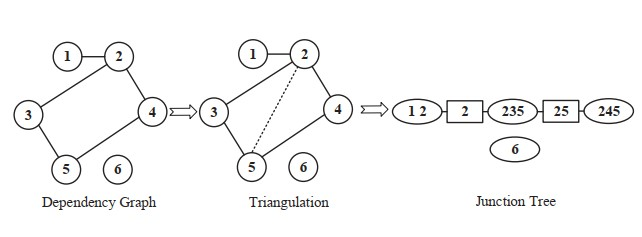
\includegraphics[width=0.9\textwidth]{figs/building_junction_tree.jpg}
  \caption{ساخت درخت اتصال از گراف همبستگی. برگرفته از \مرجع{ren2018textsf}}
  \label{fig:junctionTree}
\end{figure}

در گام چهارم  مجموعه داده مصنوعی تولید می‌شود. هدف انتشار یک مجموعه داده کاملاً جدید و مصنوعی است که از نظر آماری شبیه به داده‌های اصلی باشد اما حاوی اطلاعات هیچ کاربر واقعی نباشد. کارپذیر با استفاده از توزیع احتمال مشترکی که برای هر خوشه در گام‌های قبل محاسبه کرده، شروع به تولید رکوردهای جدید و مصنوعی می‌کند. این رکوردهای مصنوعی برای هر خوشه با هم ترکیب شده و رکوردهای کامل با ابعاد بالا را می‌سازند.

خروجی نهایی، یک مجموعه داده مصنوعی است که می‌توان آن را با خیال راحت برای تحلیل و داده‌کاوی منتشر کرد، زیرا ضمن حفظ الگوهای کلی داده‌های اصلی، حریم خصوصی تک‌تک مشارکت‌کنندگان را به طور کامل حفظ کرده است. به طور خلاصه، لوپاب به کاربران اجازه می‌دهد در پروژه‌های جمع‌سپاری داده با ابعاد بالا شرکت کنند، بدون آنکه نگران افشای اطلاعات شخصی خود، حتی به کارپذیر جمع‌آوری‌کننده، باشند.

\زیرزیرقسمت{پژوهش ماتاموروس و همکاران}

پژوهش ماتاموروس و همکاران \مرجع{HernandezMatamoros2024ComparativeAO} راهکار خود را در حوزه حریم خصوصی تفاضلی محلی برای حفاظت از داده‌های حساس، به ویژه در بخش مراقبت‌های بهداشتی، ارائه می‌دهد. مشکل داده‌های با ابعاد بالا به خصوص در داده‌های حوزه سلامت که ویژگی‌های متعددی با همبستگی بالا دارند (مانند سوابق پزشکی و نتایج آزمایش‌ها)، بسیار مشهود است. محققان برای غلبه بر این چالش‌ها، استفاده از «رگرسیون بیزی خطی\پانویس{Bayesian Ridge Regression}» را به جای روش‌های متداول پیشنهاد می‌کنند. راهکارهای قبلی مانند لوپاب از رگرسیون لاسو استفاده می‌کردند که در مواجهه با داده‌های با ابعاد بالا و همبستگی زیاد، کارایی خود را از دست می‌دهند.

محققان این پژوهش نشان می‌دهند که در مقابله با همبستگی بالا، استفاده از رگسیون بیزی خطی عملکرد بهتری داشته و با مصرف کمتر بودجه‌ی حریم خصوصی سودمندی بهتری کسب می‌شود.

\زیرزیرقسمت{پژوهش ژانگ و همکاران}

پژوهش ژانگ و همکاران \مرجع{zhang2023publishing} روشی به اسم \مهم{پرایو‌پی‌جِی}\پانویس{PrivPJ} ارائه می‌دهد که برای حفظ حریم خصوصی در هنگام انتشار داده‌های با ابعاد بالا کاربرد دارد. این روش به گونه‌ای طراحی شده است که ضمن محافظت از اطلاعات خصوصی کاربران، داده‌های مصنوعی تولید کند که از نظر آماری شباهت زیادی به داده‌های واقعی داشته باشند. روش پرایو‌پی‌جِی برای غلبه بر مشکلات داده‌های با ابعاد بالا در یک فرایند سه مرحله‌ای طراحی شده است.

مرحله‌ی اول مانند روش لوپاب، شامل آشفته‌سازی داده‌ها به صورت محلی می‌باشد. البته به جای ارسال تمام اطلاعات یک کاربر، به صورت تصادفی فقط یکی از ویژگی‌ها را انتخاب می‌کند. سپس اطلاعات این ویژگی انتخاب شده با استفاده از یک تکنیک پاسخ تصادفی نوفه‌دار می‌شود. این کار تضمین می‌کند که کارپذیر هرگز مقدار واقعی را به طور قطعی دریافت نمی‌کند. در نتیجه هر کاربر فقط یک گزارش کوچک و نوفه‌دار شده به کارپذیر ارسال می‌کند. این کار هم هزینه ارتباطی را کاهش می‌دهد و هم حریم خصوصی تفاضلی محلی را تضمین می‌کند.

در مرحله دوم تخمینی از توزیع مشترک داده‌ها تهیه می‌گردد.  پس از اینکه کارپذیر گزارش‌های نوفه‌دار شده را از تمام کاربران دریافت کرد، از الگوریتم جدیدی به نام خودکدگذار چند متغیره\پانویس{Multivariate Variational Autoencoder} (به اختصار اِم.وی.اِی.ای\پانویس{mVAE}) به منظور تخمین توزیع مشترک داده‌ها استفاده می‌کند. این الگوریتم یک مدل یادگیری عمیق است که می‌تواند توزیع احتمال مشترک بین تمام ویژگی‌ها را تخمین بزند. به بیان دیگر با تحلیل داده‌های آشفته شده، الگوها و همبستگی‌های بین ویژگی‌های مختلف را یاد می‌گیرد. این کار با به حداقل رساندن خطا بین توزیع حاشیه‌ای و توزیع مشترک انجام می‌شود و به طور موثر اثر نوفه را کاهش می‌دهد.

در مرحله سوم کاهش ابعاد و تولید داده مصنوعی صورت می‌گیرد. اکنون که کارپذیر مدل آماری داده‌ها را در اختیار دارد، باید از آن برای تولید یک مجموعه داده مصنوعی جدید استفاده کند. از آنجایی که کار با توزیع کامل داده‌های با ابعاد بالا همچنان پیچیده است، پرایو‌پی‌جِی از شبکه مارکوف\پانویس{Markov Network} برای ساده‌سازی این فرآیند استفاده می‌کند.

ساخت شبکه مارکوف به این صورت است که  ابتدا، کارپذیر با استفاده از اطلاعات همبستگی که در مرحله قبل به دست آورده، یک شبکه مارکوف می‌سازد. در این شبکه، هر ویژگی یک گره است و بین ویژگی‌هایی که همبستگی بالایی دارند، یک یال کشیده می‌شود. در قدم بعدی، شبکه مارکوف به ساختاری ساده‌تر به نام درخت اتصال تبدیل می‌شود. فرایند ساخت درخت اتصال مانند روش لوپاب است. شکل \رجوع{fig:PrivPJ} یک مثال از شبکه مارکوف و ساخت درخت اتصال را نمایش می‌دهد. این درخت، ویژگی‌ها را در خوشه‌هایی که همبستگی بالایی با هم دارند گروه‌بندی می‌کند. این کار به طور موثری ابعاد داده را کاهش می‌دهد. در نهایت، سرور از این درخت اتصال برای تولید داده‌های مصنوعی جدید استفاده می‌کند. این فرآیند با نمونه‌برداری از خوشه‌ها، روابط آماری پیچیده در داده‌های اصلی را بازسازی می‌کند.

\begin{figure}[h]
  \centering
  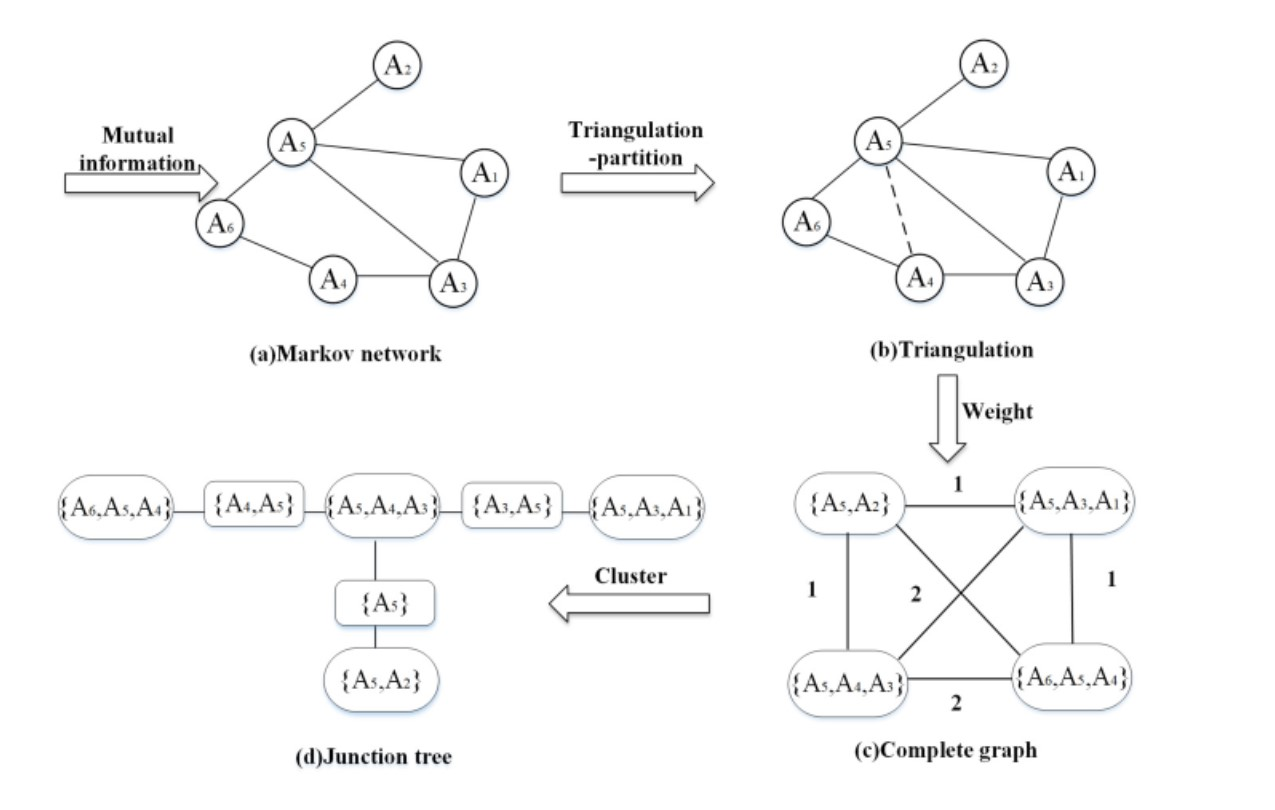
\includegraphics[width=0.9\textwidth]{figs/PrivPJ_Markov.jpg}
  \caption{استفاده از شبکه مارکوف در ساخت درخت اتصال. برگرفته از \مرجع{zhang2023publishing}}
  \label{fig:PrivPJ}
\end{figure}

نتیجه نهایی یک مجموعه داده با ابعاد بالا است که از نظر آماری بسیار شبیه به داده‌های اصلی است، اما چون از ابتدا بر پایه گزارش‌های آشفته ‌شده ساخته شده، حریم خصوصی هیچ‌یک از کاربران را نقض نمی‌کند.

\زیرزیرقسمت{پژوهش جیانگ و همکاران}

پژوهش جیانگ و همکاران \مرجع{jiang2023dp2}، راهکاری نوآورانه به نام دی.پی.تو.پاب\پانویس{DP2-Pub} به منظور حل چالش داده‌های با ابعاد بالا ارائه می‌دهد. هدف اصلی، به اشتراک گذاشتن این داده‌ها برای تحلیل و یادگیری ماشین است، بدون آنکه حریم خصوصی افراد در معرض خطر قرار گیرد. این راهکار در دو فاز اصلی و برای دو حالت متفاوت یعنی کارپذیر قابل اعتماد و کارپذیر نیمه‌صادق انجام می‌شود. 

در فاز اول خوشه‌بندی صفات انجام می‌شود. به جای کار با تمام ابعاد به صورت یکجا، ابتدا صفات مرتبط به هم را در گروه‌های کوچک‌تر و کم‌تعدادتر خوشه‌بندی می‌کند. در فاز دوم روی داده‌های هر خوشه، فرآیند افزودن نویز را برای تضمین حریم خصوصی اجرا می‌کند. 

این فرآیند در دو مدل امنیتی مختلف ارائه می‌شود:

\شروع{شمارش}

\فقره کارپذیر قابل اعتماد: در این مدل، فرض بر این است که یک کارپذیر مرکزی به داده‌های اصلی دسترسی دارد و تمام عملیات حفظ حریم خصوصی روی آن انجام می‌شود. به منظور خوشه‌بندی صفات از شبکه بیزی\پانویس{Bayesian Network} استفاده می‌شود. الگوریتم با استفاده از روش حریم خصوصی تفاضلی، یک شبکه بیزی از روی داده‌ها می‌سازد. این شبکه وابستگی‌ها و روابط شرطی بین تمام صفات را مدل می‌کند. به عنوان مثال در شکل \رجوع{fig:dp2pub} یک شبکه‌ی بیزی از پنج ویژگی ساخته می‌شود.

\begin{figure}[h]
  \centering
  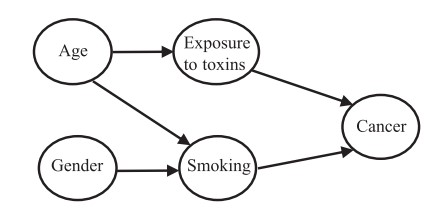
\includegraphics[width=0.9\textwidth]{figs/dp2pub_bayesian.jpg}
  \caption{ساخت شبکه بیزی از پنج ویژگی. برگرفته از \مرجع{jiang2023dp2}}
  \label{fig:dp2pub}
\end{figure}

پس از ساخت شبکه، برای هر صفت، «پوشش مارکوف\پانویس{Markov Blanket}» آن شناسایی می‌شود. پوشش مارکوف یک صفت، مجموعه‌ای حداقلی از صفات همسایه آن است که تمام اطلاعات لازم برای پیش‌بینی آن صفت را در خود دارد \مرجع{Yu2017MarkovBF}. الگوریتم با گروه‌بندی هر ویژگی به کمک پوشش مارکوف، داده‌های با ابعاد بالا را به چندین خوشه کم‌بعد و مستقل از هم تقسیم می‌کند.

\شروع{تعریف}[پوشش مارکوف]

در یک شبکه بیزی، پوشش مارکوف برای یک گره $x$، مجموعه‌ای از گره‌هاست که از نظر احتمالی، $x$ را از بقیه شبکه محافظت یا جدا می‌کنند. به این معنا که اگر مقادیر گره‌های موجود در پوشش مارکوف را بدانیم، گره $x$ از تمام گره‌های دیگر شبکه مستقل می‌شود.

\begin{equation}
MB(x) = Pa(x) \cup Ch(x) \cup \{Pa(y)|y \in Ch(x)\}
\end{equation}

در عبارت بالا:
\شروع{فقرات}

\فقره $MB(x)$: پوشش مارکوف گره $x$.
\فقره $Pa(x)$: مجموعه گره‌های والد گره $x$.
\فقره $Ch(x)$: مجموعه گره‌های فرزند گره $x$.

\پایان{فقرات}

\برچسب{تعریف: پوشش مارکوف}
\پایان{تعریف}

پس از خوشه‌بندی، باید روی داده‌ها آشفته‌سازی انجام شود. البته لازم است که کمترین آسیب به اطلاعات آماری کلان وارد شود. پژوهش الگوریتمی نوآورانه به نام پی.آر.اِی.اِم\پانویس{PRAM} ارائه می‌کند. در این روش، مقادیر داده‌ها با یک احتمال مشخص به مقادیر دیگر تغییر می‌کنند. نکته‌ی مهم این است که الگوریتم پی.آر.اِی.اِم تضمین می‌کند که توزیع آماری کلی داده‌ها پس از افزودن نوفه، بدون تغییر باقی بماند. این کار باعث حفظ حداکثری کارایی داده می‌شود. به طور دقیق‌تر، ابتدا یک بار داده‌ها را با نوفه استاندارد آشفته می‌کند. سپس، با تخمین توزیع اصلی از روی داده‌های نوفه‌دار شده، یک آشفتگی دوم و معکوس اعمال می‌کند تا اثرات منفی نوفه بر توزیع کلی را خنثی کند.

\فقره کارپذیر نیمه‌صادق: در این مدل، کاربران به کارپذیر اعتماد ندارند و می‌خواهند داده‌هایشان قبل از ارسال به کارپذیر، تصادفی‌سازی شود. هر کاربر ابتدا روی داده‌های خود یک فرآیند تصادفی‌سازی اعمال می‌کند تا داده‌هایش به صورت محلی آشفته شوند. سپس این داده‌های نوفه‌دار شده را به کارپذیر ارسال می‌کند. کارپذیر داده‌ها را از تمام کاربران جمع‌آوری کرده و سپس همان فرآیند دو فازی یعنی خوشه‌بندی و  پی.آر.اِی.اِم را روی این داده‌ها اجرا می‌کند تا همبستگی‌ها را بازسازی کرده و کارایی نهایی داده‌ها را بهبود بخشد.

\پایان{شمارش}

\زیرزیرقسمت{پژوهش دیو و همکاران}

پژوهش دیو و همکاران \مرجع{du2021collecting} الگوریتمی ارائه می‌دهد که هم حریم خصوصی کاربران حفظ شود و هم داده‌های جمع‌آوری شده کیفیت و کارایی بالایی داشته باشند. روش‌های قدیمی فرض می‌کنند که تمام ویژگی‌های داده کاملاً به هم مرتبط هستند (بدترین حالت ممکن)، در حالی که در دنیای واقعی اینطور نیست. برای مثال، دمای یک اتاق و میزان روشنایی آن ممکن است همبستگی داشته باشند، اما این همبستگی کامل و صددرصدی نیست. این پژوهش نشان می‌دهد که اگر بتوانیم میزان همبستگی بین ویژگی‌های مختلف را اندازه‌گیری کنیم، می‌توانیم نوفه را به شکل هوشمندانه‌تر و بهینه‌تری توزیع کرده و کیفیت نهایی داده‌ها را به شدت افزایش دهیم. یک پروتکل جدید به نام آشفتگی محدود به همبستگی\پانویس{Correlation-Bounded Perturbation} (به اختصار، سی.بی.پی\پانویس{CBP}) معرفی می‌گردد. این پروتکل بر اساس یک مدل حریم خصوصی جدید و منعطف‌تر به نام حریم خصوصی تفاضلی محلی با تسلط تک‌متغیره\پانویس{Univariate Dominance LDP} کار می‌کند. 

این مدل یک نسخه انعطاف‌پذیرتر از حریم خصوصی تفاضلی محلی است که به طور خاص برای یک ویژگی واحد در داده‌های با ابعاد بالا طراحی شده است. به زبان ساده، این مدل تضمین می‌کند که اگر مقدار واقعی یک ویژگی را تغییر دهیم، احتمال اینکه الگوریتم یک خروجی نوفه‌دار شده‌ی مشخص تولید کند، تفاوت چندانی نخواهد کرد. این عدم قطعیت باعث می‌شود که یک مهاجم با دیدن خروجی، نتواند با اطمینان بگوید که مقدار اصلی چه بوده است.

\شروع{تعریف}[حریم خصوصی تفاضلی محلی با تسلط تک‌متغیره]

برای هر ویژگی دلخواه $x$ و برای هر دو ورودی ممکن $s$ و $s'$، سازوکار $M$، شرایط حریم خصوصی تفاضلی محلی با تسلط تک‌متغیره را برآورده می‌کند، اگر برای هر خروجی ممکن $Y$ از دامنه سازوکار $M$، شرط زیر برقرار باشد:

\begin{equation}
e^{-\epsilon} \le \frac{P[\mathcal{M}(x = s) = Y]}{P[\mathcal{M}(x = s') = Y]} \le e^{\epsilon}
\end{equation}

\برچسب{حریم خصوصی تفاضلی محلی با تسلط تک‌متغیره}
\پایان{تعریف}

کارپذیر با استفاده از داده‌های تاریخی یا دانش قبلی، ویژگی‌هایی را که به هم مرتبط هستند، شناسایی و دسته‌بندی می‌کند. سپس به جای تقسیم مساوی بودجه حریم خصوصی، پروتکل سی.بی.پی این بودجه را به صورت هوشمندانه بر اساس میزان همبستگی بین ویژگی‌ها تخصیص می‌دهد. ویژگی‌هایی که همبستگی بیشتری دارند، می‌توانند به شکل مؤثرتری بودجه حریم خصوصی را به اشتراک بگذارند.

در بسیاری از کاربردهای اینترنت اشیاء، پهنای باند یک محدودیت جدی است و نمی‌توان همیشه تمام داده‌ها را ارسال کرد. برای حل این مشکل، مقاله پروتکل سی.بی.پی را گسترش داده و از نمونه‌برداری نیز استفاده می‌کند. به این صورت که نه تنها بودجه حریم خصوصی را بهینه تخصیص می‌دهد، بلکه احتمال نمونه‌برداری از هر ویژگی را نیز بر اساس میزان اهمیت و همبستگی آن تعیین می‌کند. این کار باعث می‌شود که حتی با ارسال تعداد محدودی از ویژگی‌ها، بیشترین اطلاعات ممکن با حفظ حریم خصوصی استخراج شود.

از مشکلات این پژوهش می‌توان به این نکته اشاره کرد که وجود داده‌های تاریخی یا دانش قبلی همیشه میسر نخواهد بود. اگر این دانش را نداشته باشیم، نمی‌توانیم میزان همبستگی بین ابعاد داده را محاسبه کنیم و در نتیجه خوشه‌بندی مناسبی نخواهیم داشت.

\زیرزیرقسمت{پژوهش گوهوا شِن و همکاران}

پژوهش گوهوا شِن و همکاران \مرجع{Shen2024LoHDPAL} نیز مانند پژوهش‌های پیشین راهکاری مبتنی بر خوشه‌بندی برای انتشار داده‌های چندبُعدی ارائه می‌دهد که حریم خصوصی افراد را با استفاده از روش حریم خصوصی تفاضلی محلی حفظ می‌کند. ایده اصلی این راهکار بر دو بخش استوار است.

ابتدا محاسبه‌ی توزیع حاشیه‌ای انجام می‌شود. به جای تقسیم بودجه حریم خصوصی که باعث کاهش دقت می‌شود، این روش از تکنیک‌های مبتنی بر نمونه‌گیری برای افزودن نوفه به داده‌های کاربران استفاده می‌کند. سپس به صورت هوشمند و انطباقی، توزیع حاشیه‌ای از ویژگی‌های داده را محاسبه می‌کند. این کار به کارپذیر اجازه می‌دهد تا الگوهای آماری مهم را با دقت بیشتری تخمین بزند.

سپس ویژگی‌ها به صورت مؤثر خوشه‌بندی می‌شوند. این راهکار با یک روش کارآمد، میزان ارتباط و وابستگی بین ویژگی‌های مختلف داده را اندازه‌گیری می‌کند. سپس ویژگی‌های مرتبط را در خوشه‌هایی دسته‌بندی کرده و با استفاده از شبکه مارکوف، این ارتباطات را مدل‌سازی می‌نماید. در نهایت، کارپذیر مرکزی با استفاده از توزیع‌های آماری و خوشه‌های به‌دست‌آمده، یک مجموعه داده مصنوعی تولید می‌کند. 

\زیرزیرقسمت{پژوهش کیکوچی و همکاران}

پژوهش کیکوچی و همکاران \مرجع{Kikuchi2024PrivacyPreservingCF} نیز از خوشه‌بندی استفاده کرده تا چالش موجود در داده‌های با ابعاد بالا را حل کند. ابتدا به جای تحلیل تمام ابعاد داده به صورت یکجا، ویژگی‌های مرتبط و وابسته به یکدیگر را در خوشه‌های کوچکتر دسته‌بندی می‌کند. وابستگی میان صفات بدون افشای مقادیر اصلی و خصوصی داده‌ها تخمین زده می‌شود. در نهایت نوفه بر اساس خوشه‌ها تزریق می‌شود.

\زیرزیرقسمت{پژوهش سانگ و همکاران}

پژوهش سانگ و همکاران \مرجع{Song2024MultiDimensionalDC} راهکار خود را برای جمع‌آوری داده‌های چند‌بُعدی به این صورت بیان می‌کند که ابتدا خوشه‌بندی انجام شود و سپس مقدار نوفه بر اساس این خوشه‌بندی بهینه شود. این تحقیق در ابتدا سازوکار‌های جدیدی برای جمع‌آوری داده‌های عددی ارائه می‌دهد که دقت بالاتری نسبت به راهکارهای موجود دارند و واریانس نوفه در آن‌ها کمتر است. سپس، این سازوکارها برای داده‌های چندبعدی که شامل هر دو نوع داده‌های عددی و غیر عددی هستند، گسترش داده می‌شوند.


\زیرقسمت{کاهش ابعاد}

در بعضی از پژوهش‌هایی که قبل‌تر ذکر کردیم نیز کاهش ابعاد صورت می‌گرفت. برای مثال، خوشه‌بندی موجب کاهش ابعاد داده می‌شود. پژوهش‌هایی هم وجود دارند که خوشه‌بندی انجام نداده‌اند ولی به نوعی ابعاد داده را کاهش داده‌اند تا بودجه‌ی حریم خصوصی به صورت مناسب پخش شود.

\زیرزیرقسمت{پژوهش دونگیو ژانگ و همکاران}

پژوهش دونگیو ژانگ و همکاران \مرجع{Zhang2023LocallyDP} یک راهکار نوآورانه به نام \مهم{پی.پی.اِم.سی}\پانویس{PPMC} برای جمع‌آوری داده‌های چندبعدی با حفظ حریم خصوصی تفاضلی محلی ارائه می‌دهد.پژوهش برای غلبه بر این چالش داده‌های با ابعاد بالا، یک فرآیند هوشمندانه سه مرحله‌ای را با استفاده از \مهم{تبدیل هار}\پانویس{Haar Transform} پیشنهاد می‌کند. شکل \رجوع{fig:PPMC} این سه مرحله را به خوبی نمایش می‌دهد. ایده اصلی این است که به جای افزودن نوفه به تک‌تک ابعاد داده‌ی اصلی، ابتدا ساختار داده را تغییر داده، ابعاد آن را کاهش دهیم و سپس به داده‌ی تبدیل‌شده نوفه اضافه کنیم.

\begin{figure}[h]
  \centering
  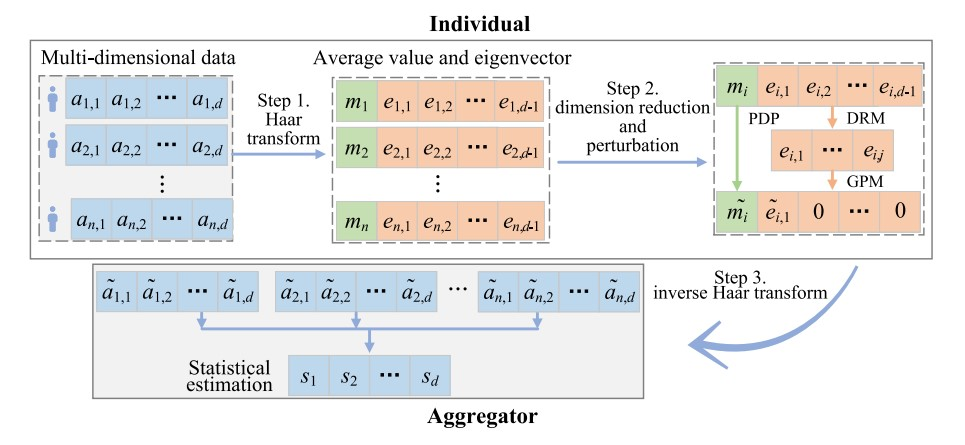
\includegraphics[width=0.9\textwidth]{figs/PPMC.jpg}
  \caption{ساختار روش پی.پی.اِم.سی. برگرفته از \مرجع{Zhang2023LocallyDP}}
  \label{fig:PPMC}
\end{figure}

تبدیل هار یکی از قدیمی‌ترین، ساده‌ترین و در عین حال بنیادی‌ترین ابزارهای ریاضی در خانواده تبدیل‌های موجک\پانویس{Wavelet Transforms} است. این تبدیل، یک سیگنال یا مجموعه‌ای از داده‌ها (مانند یک تصویر یا یک فایل صوتی) را به دو بخش اصلی تجزیه می‌کند:

\شروع{فقرات}

\فقره اطلاعات کلی

\فقره اطلاعات جزئی

\پایان{فقرات}

به بیان دیگر تبدیل هار یک تبدیل خطی است که سیگنال یا ورودی خاص را را به نمایشی تبدیل می‌کند که الگوها و جزئیات داده را در مقیاس‌های مختلف برجسته می‌کند. در رابطه با کاربرد این تبدیل در حریم خصوصی تفاضلی محلی، تبدیل هار، داده‌ها را به دو بخش اصلی تجزیه می‌کند:

\شروع{فقرات}

\فقره مقدار میانگین\پانویس{Average Value}: این یک مقدار واحد است که یک تقریب کلی و چکیده از تمام ابعاد داده را در خود نگه می‌دارد. بخش عمده‌ای از اطلاعات مهم داده‌ها در همین مقدار میانگین متمرکز می‌شود.

\فقره بردار ویژه\پانویس{Eigenvector}: این بردار، اطلاعات جزئی‌تر و تفاوت‌های بین ابعاد مختلف را نشان می‌دهد. این مقادیر معمولاً کوچک‌تر هستند و اطلاعات کمتری نسبت به مقدار میانگین در خود دارند.

\پایان{فقرات}

مزیت کلیدی این کار این است به جای داشتن تعداد زیادی بُعد که همگی به یک اندازه مهم به نظر می‌رسند، ما یک «مقدار میانگین» بسیار مهم و یک «بردار ویژه» با اهمیت کمتر داریم. این‌ها پایه و اساس کاهش ابعاد را فراهم می‌کنند. در ادامه با یک مثال نحوه‌ی عملکرد این تبدیل را مشخص کنیم.

تصور کنید یک لیست از اعداد مانند $[9, 7, 3, 5, 8, 4, 5, 7]$ داریم. به راحتی با جمع تک تک اعداد و تقسیم بر تعداد آنها، مقدار میانگین را محاسبه می کنیم:

$$m = \frac{7+5+4+8+5+3+7+9}{8} = 6$$

برای محاسبه‌ی بردار ویژه، ابتدا یک درخت دودویی کامل می‌سازیم که برگ‌های درخت همان اعداد (ابعاد داده) اصلی هستند. سپس، برای هر گره داخلی $N$، مقدار ویژه $e = (ml {-} mr)/2$ محاسبه می‌شود، که در آن $ml$ و $mr$ مقدار میانگین گره‌های برگ در زیردرخت‌های چپ و راست $N$ است. پس از پردازش تمام گره‌های داخلی، با نوشتن آنها به ترتیب جستجوی اول سطح\پانویس{Breadth First Search} مقدار بردار ویژه بدست می‌آید. دقت کنید مقدار میانگین را می‌توان به عنوان اطلاعات اصلی داده‌های چند بعدی در نظر گرفت و هر مقدار ویژه را می‌توان به چشم اطلاعات محلی داده‌های چند بعدی مشاهده کرد. بنابراین، هر بعد را می‌توان به عنوان مجموعه‌ای از مقدار میانگین و مقادیر ویژه در نظر گرفت. شکل \رجوع{fig:haar_tree} تبدیل هار را روی داده‌های چند بعدی نشان می‌دهد.

$$E = [0, 2, 0, 1, -1, 2, -1]$$

\begin{figure}[h]
  \centering
  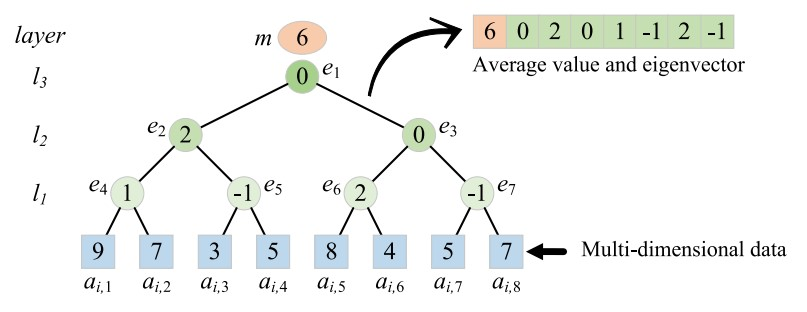
\includegraphics[width=0.9\textwidth]{figs/haar_tree.jpg}
  \caption{نحوه‌ محاسبه‌ی بردار ویژه در تبدیل هار. $a_{i,j}$ نشان‌دهنده‌ی ویژگی $j$ام از کاربر $i$ام است. برگرفته از \مرجع{Zhang2023LocallyDP}}
  \label{fig:haar_tree}
\end{figure}

نکته کلیدی: این فرآیند بازگشت‌پذیر است. یعنی با داشتن میانگین و بردار ویژه، می‌توان داده اصلی را دقیقاً بازسازی کرد. برای پیدا کردن مقدار هر داده (که در برگ‌های درخت قرار دارد)، از ریشه درخت (که همان مقدار میانگین m است) شروع کرده و با اضافه یا کم کردن مقادیر ویژه‌ای که در مسیر رسیدن به آن برگ قرار دارند، به مقدار نهایی می‌رسیم:

\begin{equation}
a_{i,j} = m + \sum_{k=1}^{l} (g_k \cdot e_k)
\label{equ:inverse_haar}
\end{equation}

$$g_k =
\begin{cases} 
1, & \text{if} \quad a_{i,j} \text{ of subtree left the in } e_k, \\[10pt]
-1, & \text{if} \quad a_{i,j} \text{ of subtree right the in } e_k.
\end{cases}$$

$$l = \lfloor \log(d+1) - 1 \rfloor$$

به عبارت دیگر، برای بازسازی یک مقدار، از میانگین کل شروع می‌کنیم و سپس در هر مرحله از مسیر درخت، مقدار ویژه آن مرحله را بر اساس اینکه در سمت چپ یا راست آن قرار داریم، اضافه یا کم می‌کنیم. به عنوان مثال در شکل \رجوع{fig:haar_tree} ویژگی $a_{i,7}$ دارای اجداد $e_7$، $e_3$ و $e_1$ است. معکوس تبدیل هار برای این ویژگی به شکل زیر محاسبه می‌شود:

$$a_{i,7} = m - e_1 - e_3 + e_7 = 5$$


همانطور که می‌بینید، مقدار بازسازی شده دقیقاً با مقدار اصلی در داده‌های خام (عدد ۵) برابر است، که نشان می‌دهد فرآیند معکوس به درستی کار می‌کند.

سادگی و سرعت محاسباتی تبدیل هار باعث شده تا در حوزه‌های مختلفی کاربرد داشته باشد:

\شروع{فقرات}

\فقره فشرده‌سازی داده‌ها\پانویس{Data Compression}: فشرده‌سازی یکی از مهم‌ترین کاربردهای تبدیل هار است. بسیاری از داده‌ها (مانند تصاویر) شامل ضرایبی با مقادیر کوچک و نزدیک به صفر هستند. با حذف این ضرایب کم‌اهمیت و نگهداری ضرایب تقریبی و بزرگ، می‌توان حجم داده را به شدت کاهش داد بدون اینکه کیفیت آن به طور محسوس افت کند. فرمت تصویر \lr{JPEG} از نسخه‌های پیشرفته‌تر موجک‌ها (که بر پایه همین ایده هستند) استفاده می‌کند.

\فقره تشخیص لبه\پانویس{Edge Detection}: ضرایب جزئی در یک تصویر، نماینده تغییرات ناگهانی روشنایی هستند که دقیقاً همان لبه‌های اشیاء را مشخص می‌کنند.

\فقره کاهش نوفه\پانویس{Denoising}: نوفه در تصویر معمولاً به صورت ضرایب جزئی کوچک ظاهر می‌شود. با حذف این ضرایب و بازسازی تصویر، می‌توان نوفه را تا حد زیادی از بین برد.

\فقره تحلیل سیگنال‌های دیجیتال: برای بررسی و تحلیل فرکانس‌های مختلف در سیگنال‌های صوتی یا دیگر سیگنال‌های دیجیتال استفاده می‌شود.

\فقره پایگاه داده: برای جستجوی سریع‌تر و بهینه در پایگاه داده‌های بزرگ به کار می‌رود.

\پایان{فقرات}

به طور خلاصه، تبدیل هار یک ابزار قدرتمند برای تجزیه داده‌ها به بخش‌های کلی و جزئی است که این ویژگی آن را برای کاربردهای متنوعی از فشرده‌سازی گرفته تا حفظ حریم خصوصی، بسیار مفید می‌سازد. پژوهش \مرجع{Zhang2023LocallyDP} در سه مرحله چالش حفظ حریم خصوصی برای داده‌های با ابعاد بالا را حل کرده است:

اولین و مهم‌ترین قدم، استفاده از تبدیل هار برای تبدیل داده‌های چندبعدی هر کاربر است. 

در مرحله‌ی بعد حفاظت از حریم خصوصی داده‌های تبدیل‌شده صورت می‌گردد. اکنون به جای کار با داده خام، الگوریتم روی دو بخش تبدیل‌شده کار می‌کند و برای هر کدام، یک سازوکار بهینه‌سازی‌شده برای افزودن نوفه ارائه می‌دهد:

\شروع{فقرات}

\فقره حفاظت از مقدار میانگین:  برای محافظت از مقدار میانگین، مقاله یک سازوکار به نام آشفته‌سازی مبتنی بر چگالی احتمال\پانویس{Probability Density-based Perturbation} (به اختصار، \مهم{پی.دی.پی}\پانویس{PDP}) طراحی کرده است. این سازوکار به جای افزودن نوفه‌ی کاملاً تصادفی، به صورت هوشمندانه عمل می‌کند. مقدار نوفه به گونه‌ای اضافه می‌شود که مقدار نهایی با احتمال بالاتری نزدیک به مقدار واقعی باقی بماند و با احتمال کمتری از آن دور شود. این کار باعث می‌شود که با حفظ حریم خصوصی، دقت و کارایی این مقدار کلیدی تا حد امکان حفظ شود. به طور دقیق‌تر، مقدار نوفه‌دار شده‌ی $\tilde{m} \in [-b,b]$ از رابطه‌ی زیر بدست می‌آید.

\begin{equation}
\text{PDF}[\psi(m) = \tilde{m}] = 
\begin{cases} 
q \cdot e^{\epsilon} & \text{if } \quad \tilde{m} \in L(\Delta, m), \\
q & \text{otherwise},
\end{cases}
\end{equation}

در عبارت بالا $q$ یک مقدار ثابت است که باعث می‌شود مجموع همه احتمالات در تابع چگالی احتمال برابر با 1 شود. پارامترهای دیگر عبارت به صورت زیر بهینه سازی می‌شوند:
$$L(\delta, m) = \left[m - \frac{\delta}{2}, m + \frac{\delta}{2}\right]$$
$$\Delta = \frac{24}{e^{\epsilon/6}(6+5\epsilon)-6}$$
$$b = \frac{(e^{\epsilon}-1)\Delta(\Delta+2)}{2[(e^{\epsilon}-1)\Delta-2]}$$
$$q = \frac{2}{(e^{\epsilon}-1)\Delta(2b-\Delta)}$$

در شکل \رجوع{fig:PDP} مثالی از آشفته‌سازی مقدار میانگین نمایش داده شده است.

\begin{figure}[h]
  \centering
  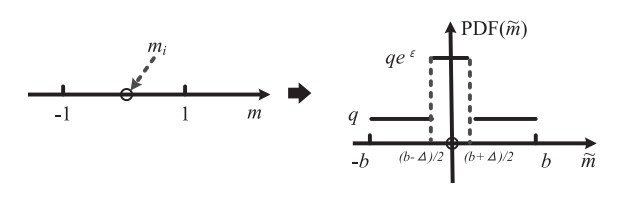
\includegraphics[width=0.9\textwidth]{figs/PDP.jpg}
  \caption{آشفته‌سازی مقدار $m_i$ بر اساس پی.دی.پی. برگرفته از \مرجع{Zhang2023LocallyDP}}
  \label{fig:PDP}
\end{figure}

\فقره حفاظت از بردار ویژه: برای این بخش که هنوز چندبعدی است، ابتدا کاهش ابعاد صورت می‌گیرد. از آنجایی که بسیاری از مقادیر در بردار ویژه کوچک و کم‌اهمیت هستند، این مدل مقادیری را که از یک آستانه مشخصی کوچک‌تر هستند، حذف کرده و آن‌ها را با صفر جایگزین می‌کند. سپس از سازوکاری به اسم آشفته‌سازی سراسری\پانویس{Global Perturbation Mechanism} (به اختصار \مهم{جی.پی.اِم}\پانویس{GPM}) به منظور اضافه کردن نوفه به بردار ویژه استفاده می‌شود. به جای تقسیم بودجه حریم خصوصی بین ابعاد باقی‌مانده‌ی بردار ویژه، این نوفه کل بردار را به عنوان یک واحد در نظر گرفته و به صورت سراسری به آن نوفه اضافه می‌کند. این رویکرد از تقسیم بیش از حد بودجه جلوگیری کرده و کارایی آماری را به مراتب بهتر حفظ می‌کند. رویکرد اضافه کردن نوفه به بردار ویژه در الگوریتم \رجوع{الگوریتم: سازوکار آشفته‌سازی بردار ویژه} نوشته شده است.

ابتدا کاهش ابعاد با استفاده از حد آستانه (خطوط ۱ تا ۵) انجام می‌شود. این مرحله یک پیش‌پردازش برای بهینه‌سازی است. الگوریتم تک‌تک مقادیر داخل بردار ویژه را بررسی می‌کند. اگر قدر مطلق یک مقدار از آستانه $\theta$ کوچک‌تر باشد، آن را با صفر جایگزین می‌کند. مقادیر بسیار کوچک در بردار ویژه، اطلاعات کمی را در خود دارند اما همچنان بخشی از بودجه حریم خصوصی را مصرف می‌کنند. با حذف (صفر کردن) آن‌ها، الگوریتم می‌تواند بودجه حریم خصوصی را برای محافظت از مقادیر مهم‌تر متمرکز کند.

سپس یک بردار دودویی به نام $\tilde{V}$ ایجاد می‌شود. این بردار مشخص می‌کند که به هر بعد از بردار ویژه چه نوع نوفه‌ای اضافه شود. نکته هوشمندانه اینجاست که خودِ این بردار $\tilde{V}$ به روشی انتخاب می‌شود که حریم خصوصی را تضمین کند. الگوریتم دو مجموعه از بردارهای ماسک را تعریف می‌کند:

\شروع{فقرات}

\فقره مجموعه $A$: تمام بردارهای ماسک ممکنی که تعداد زوجی از عدد 1 دارند.

\فقره مجموعه $B$: تمام بردارهای ماسک ممکنی که تعداد فردی از عدد ۱ دارند.

\پایان{فقرات}

سپس با یک پرتاب سکه (متغیر $X$) که احتمال آن به بودجه حریم خصوصی $\epsilon$ بستگی دارد، تصمیم می‌گیرد که بردار ماسک نهایی را از مجموعه $A$ انتخاب کند یا از مجموعه $B$. به بیان دیگر حفظ حریم خصوصی از عدم قطعیتی ناشی می‌شود که ناظر خارجی نمی‌داند ماسک نهایی از کدام مجموعه انتخاب شده است. اکنون که بردار ماسک انتخاب شده است، نوبت به افزودن نوفه به مقادیر بردار ویژه می‌رسد.

الگوریتم به ازای هر مقدار $e_i$ از بردار ویژه، به بیت متناظر آن در بردار ماسک نگاه می‌کند. اگر بیت متناظر برابر ۰ بود، مقدار $e_i$ با انتخاب یک عدد تصادفی از بازه توزیع یکنواخت باریک، نوفه‌دار می‌شود. در غیر این صورت مقدار $e_i$ با انتخاب یک عدد تصادفی از یک بازه‌ی پهن‌تر، نوفه‌دار می‌شود. بازه این توزیع‌ها به دقت و بر اساس بودجه حریم خصوصی طراحی شده‌اند تا کل فرآیند، حریم خصوصی تفاضلی محلی را برآورده کند.

\شروع{الگوریتم}{سازوکار آشفته‌سازی بردار ویژه}
\ورودی بردار ویژه‌ی  $e_i \in [-1, 1]^{d-1}$ و بودجه‌ی حریم خصوصی $\epsilon_2$ و حد آستانه‌ی $\theta$.
\خروجی مقدار نوفه‌دار شده‌ی $\tilde{e}_i \in [-\frac{e^{\epsilon}+1}{e^{\epsilon}-1}, \frac{e^{\epsilon}+1}{e^{\epsilon}-1}]^{d-1}$

\For{هر $e_i$ از بردار ویژه}
    \If{$|e_i| \leq \theta$}
        \State $e_i = 0$
    \EndIf
\EndFor
\دستور $V = \{0\}^{d-1-\theta d}$
\دستور به صورت تصادفی $k$ بیت از لیست $V$ را 1 قرار بده.
\دستور قرار بده $A$ را برابر با لیست‌هایی که $k$ی آنها زوج است.
\دستور قرار بده $B$ را برابر با لیست‌هایی که $k$ی آنها فرد است.
\دستور یک متغیر برنولی $X$ را با احتمال $\frac{e^{\epsilon}}{e^{\epsilon}+1}$ مقدار 1 قرار بده.

\If{$X = 1$}
    \دستور لیست $\tilde{V}$ را به صورت تصادفی یکنواخت از $A$ انتخاب کن.
\Else
    \دستور لیست $\tilde{V}$ را به صورت تصادفی یکنواخت از $B$ انتخاب کن.
\EndIf
\For{هر $e_i$ از بردار ویژه}
    \If{$v_i = 0$}
        \دستور مقدار $\tilde{e}_i$ را به صورت تصادفی یکنواخت از $[\frac{e_i \cdot e^{\epsilon}-1}{e^{\epsilon}-1}, \frac{e_i \cdot e^{\epsilon}+1}{e^{\epsilon}-1}]$ انتخاب کن.
    \Else
        \دستور مقدار $\tilde{e}_i$ را به صورت تصادفی یکنواخت از $[-\frac{e^{\epsilon}+1}{e^{\epsilon}-1}, \frac{e_i \cdot e^{\epsilon}-1}{e^{\epsilon}-1}) \cup (\frac{e_i \cdot e^{\epsilon}+1}{e^{\epsilon}-1}, \frac{e^{\epsilon}+1}{e^{\epsilon}-1}]$ انتخاب کن.
    \EndIf
\EndFor
\دستور $\tilde{e}_i \in [-\frac{e^{\epsilon}+1}{e^{\epsilon}-1}, \frac{e^{\epsilon}+1}{e^{\epsilon}-1}]^{d-1}$ را برگردان

\پایان{الگوریتم}

\پایان{فقرات}

در مرحله سوم بازسازی داده‌ها شکل می‌گیرد. پس از اینکه هر کاربر مقدار میانگین و بردار ویژه‌ی نوفه‌دار شده‌ی خود را ارسال کرد، کارپذیر با استفاده از تبدیل معکوس هار \رجوع{equ:inverse_haar}، این دو قطعه اطلاعات را با هم ترکیب کرده و یک نسخه‌ی تقریبی از داده چندبعدی اصلی را بازسازی می‌کند. نکته مهم این است که کارپذیر هرگز به داده‌های خام و اصلی کاربران دسترسی نداشته و تمام فرآیند بازسازی بر اساس داده‌های نوفه‌دار شده انجام می‌شود که حریم خصوصی آن‌ها تضمین شده است. این رویکرد باعث می‌شود که داده‌های جمع‌آوری‌شده با وجود حفظ حریم خصوصی، کارایی آماری بسیار بالاتری نسبت به روش‌های قبلی داشته باشند.

\قسمت{داده‌های در حال تغییر}

در اکثر اوقات، نیاز به جمع‌آوری و تحلیل داده‌ها در طول زمان و به صورت مداوم  وجود دارد. به عنوان مثال، یک شرکت نرم‌افزاری ممکن است بخواهد آمار استفاده از یک قابلیت خاص را به صورت روزانه یا هفتگی رصد کند. این کار مستلزم پرسش‌های مکرر از داده‌های کاربران است. چالش اصلی این است که حتی اگر هر پاسخ به صورت جداگانه با استفاده از سازوکارهای حفظ حریم خصوصی محافظت شود، تکرار این فرآیند می‌تواند به مرور زمان حریم خصوصی را تضعیف کند.

یکی از بزرگترین خطرات در پرسش‌های مکرر، حملات میانگین‌گیری\پانویس{Averaging Attacks} است. در این نوع حمله، یک مهاجم با جمع‌آوری چندین پاسخ تصادفی‌شده از یک کاربر در طول زمان، می‌تواند با میانگین‌گیری از آن‌ها، نوفه‌ی اضافه شده را کاهش داده و به مقدار واقعی داده‌های کاربر نزدیک‌تر شود. این امر به ویژه زمانی خطرناک است که مقدار واقعی داده‌های کاربر در طول زمان ثابت باقی بماند.

به بیان دیگر بر اساس قضیه ترکیب متوالی در حریم خصوصی تفاضلی، هر بار که یک پرسش در مورد داده‌های یک فرد پرسیده می‌شود، مقداری از بودجه حریم خصوصی مصرف می‌شود. تکرار پرسش‌ها باعث انباشت این مصرف و در نتیجه افت حریم خصوصی می‌شود. یعنی با هر پرسش جدید، تضمین‌های حریم خصوصی ضعیف‌تر می‌شوند.

روش حفظ کردن (در قسمت بعد شرح می‌دهیم) تا حد قابل قبولی مشکل پرسش‌های مکرر را حل کرده است ولی در حوزه‌ی داده‌های در حال تغییر همچنان مشکلاتی وجود دارد. داده‌های بسیاری از کاربران در دنیای واقعی ثابت نیستند و در طول زمان تغییر می‌کنند. به عنوان مثال، موقعیت مکانی یک فرد یا میزان استفاده از یک برنامه کاربردی، همگی در حال تحول هستند. این داده‌های در حال تغییر چالش‌های منحصر به فردی را ایجاد می‌کنند:

\شروع{فقرات}

\فقره ردیابی تغییرات داده‌ها: اگر یک کاربر مقدار داده خود را تغییر دهد (مثلاً از یک مکان به مکان دیگر برود)، حتی با استفاده از روش حفظ کردن، یک پاسخ تصادفی‌شده جدید باید تولید شود. مهاجم با مشاهده این تغییر در پاسخ تصادفی‌شده، می‌تواند متوجه شود که داده‌های کاربر تغییر کرده است. اگرچه ممکن است مهاجم نتواند مقادیر دقیق قبلی و فعلی را بفهمد، اما صرفاً آگاهی از زمان و تعداد تغییرات، خود یک نوع نشت اطلاعاتی محسوب می‌شود که می‌تواند در تحلیل‌های پیشرفته‌تر مورد سوءاستفاده قرار گیرد.

\فقره افزایش خطی افت حریم خصوصی با تغییرات ریز داده: وجود تغییرات کوچک در داده باعث می‌شود قانون ترکیب متوالی در این شرایط هم صدق کرده و بدین ترتیب حریم خصوصی نقض شود. این حالت معمولا در ویژگی‌هایی که دامنه‌ی ورودی بزرگی دارند رخ می‌دهد.

\فقره یافتن الگوری تغییرات: در بعضی حالات مهاجم می‌تواند با مشاهده تطابق بین داده‌های تغییر یافته و داده‌های اصلی، الگوی تغییرات حساس داده را شناسایی کرده و اطلاعات شخصی کاربران را استنتاج نماید.

\پایان{فقرات}


\زیرقسمت{حفظ کردن}

همانطور که قبل‌تر گفتیم، در حوزه‌ی پرسش‌های مکرر، مهاجم می‌تواند از نتایج تصادفی‌سازی میانگین گرفته تا به اطلاعات شخصی کاربران نزدیک‌تر شود. دلیل وجود این مشکل هم قانون ترکیب متوالی است. به بیان دیگر، اگر برای هر بار تصادفی‌سازی، از بودجه‌ی حریم خصوصی استفاده کنیم، در نهایت بودجه‌ی محدود ما رو به اتمام می‌رود.

روش حفظ کردن\پانویس{Memoization} یک رویکرد بسیار ساده ولی کارآمد است. به این صورت که کافیست با یکبار تصادفی‌سازی داده، مقدار حاصل ذخیره شده و در صورت پرسش دوباره روی همان داده، مقدار ذخیره‌شده برگردانده شود. اینکار از مصرف چند باره‌ی بودجه‌ی حریم خصوصی جلوگیری می‌کند. همچنین سرعت اجرای سازوکار افزایش میابد زیرا برای هر داده فقط یکبار آشفته‌سازی انجام می‌شود.

\زیرزیرقسمت{پژوهش الینگسون و همکاران}

پژوهش الینگسون و همکاران\مرجع{erlingsson2014rappor} روشی به اسم رپور\پانویس{Rappor} به منظور حفظ حریم خصوصی تفاضلی محلی ارائه می‌دهد. به بیان دیگر رپور یک فناوری توسعه‌یافته توسط گوگل است که به شرکت‌ها اجازه می‌دهد آمار کلی رفتار کاربران را جمع‌آوری کنند، بدون اینکه بتوانند به اطلاعات خصوصی یک کاربر خاص دسترسی پیدا کنند. رپور دارای یک فرایند چهار مرحله‌ای است: 

\شروع{شمارش}

\فقره تبدیل داده با استفاده از بلوم فیلتر: ابتدا، داده خام کاربر توسط بلوم فیلتر به یک رشته از صفر و یک تبدیل می‌شود. این کار داده‌ها را استاندارد و غیرقابل شناسایی می‌کند.

\فقره پاسخ تصادفی دائمی\پانویس{Permanent Randomized Response}:  این مرحله کلید اصلی حفظ حریم خصوصی بلندمدت\پانویس{Longitudinal Privacy} است. سیستم یک بار و برای همیشه، روی رشته‌ی تولید شده از مرحله قبل، یک پاسخ تصادفی اعمال می‌کند. یعنی برخی از بیت‌های ۰ به ۱ و برعکس، با یک احتمال مشخص تغییر می‌کنند. نتیجه این مرحله در دستگاه کاربر ذخیره می‌شود. این ذخیره‌سازی باعث می‌شود حتی اگر کاربر بارها گزارشی درباره همان داده ارسال کند، از حملات میانگین‌گیری جلوگیری شود. به صورت دقیق‌تر، برای هر رشته‌ی $B$ تولید شده توسط بلوم فیلتر، رشته‌ی تصادفی‌سازی شده‌ی $B'$ با استفاده از سازوکار زیر تولید می‌شود:

$$B_i' = 
\begin{cases} 
1, & \text{probability with } \hspace{5pt} \frac{1}{2}f \\
0, & \text{probability with } \hspace{5pt} \frac{1}{2}f \\
B_i, & \text{probability with } \hspace{5pt} 1 - f 
\end{cases}$$

در عبارت بالا، $B_i$ نشان‌دهنده‌ی بیت $i$ام از رشته‌ی $B$ است. $f$ یک پارامتر قابل تنظیم برای کاربر است که سطح ضمانت حریم خصوصی را کنترل می‌کند. بدین ترتیب، $B'$ به عنوان پایه‌ای برای تمام گزارش‌های آینده مورد استفاده مجدد قرار می‌گیرد.

\فقره پاسخ تصادفی آنی\پانویس{Instantaneous Randomized Response}: قبل از ارسال گزارش به کارپذیر، یک بار دیگر نوفه اضافه می‌شود. این بار، روی نتیجه پاسخ تصادفی دائمی، مجدداً یک فرآیند پاسخ تصادفی اجرا می‌شود. این کار باعث می‌شود هر گزارش ارسالی، حتی برای یک داده یکسان، با گزارش قبلی متفاوت به نظر برسد. این مرحله از ردیابی کاربر بر اساس گزارش‌های متوالی جلوگیری کرده و از شفاف شدن الگوی تغییرات جلوگیری می‌کند. به طور دقیق‌تر، آرایه‌ی تمام صفر $S$ با اندازه $B'$ ساخته می‌شود. سپس هر بیت از این آرایه با احتمال زیر، 1 می‌شود:

$$P(S_i = 1) = 
\begin{cases} 
q, & \text{if } \hspace{5pt} B'_i = 1 \\ 
p, & \text{if } \hspace{5pt} B'_i = 0 
\end{cases}$$

\فقره ارسال گزارش به کارپذیر: در نهایت، این رشته بیت که دو بار دستخوش تغییر تصادفی شده، سمت کارپذیر ارسال می‌شود. گزارش نهایی برای کارپذیر به تنهایی بی‌معنی و پر از نوفه است. اما قدرت رپور زمانی مشخص می‌شود که میلیون‌ها گزارش از کاربران مختلف جمع‌آوری شود. کارپذیر با استفاده از تکنیک‌های آماری پیشرفته، می‌تواند نوفه‌های تصادفی را از داده‌های تجمیع‌شده حذف کرده و الگوهای واقعی را در سطح کل جمعیت کشف کند. برای مثال، می‌تواند بفهمد که چند درصد از کاربران از یک وب‌سایت خاص به عنوان صفحه اصلی خود استفاده می‌کنند، بدون اینکه بداند کدام کاربران این کار را انجام داده‌اند.

\پایان{شمارش}

این روش توسط گوگل در مرورگر کروم برای جمع‌آوری آمار درباره تنظیمات کاربران (مانند صفحه اصلی، موتور جستجوی پیش‌فرض و افزونه‌های نصب‌شده) استفاده شده است. همچنین گوگل می‌تواند بدون نقض حریم خصوصی، نرم‌افزارهای مخربی که این تنظیمات را بدون اجازه تغییر می‌دهند، شناسایی کند.

\زیرقسمت{رُند کردن}

پژوهش رپور فرض می‌کند که داده‌ها تغییر نکرده یا به ندرت تغییر می‌کنند. اگر اطلاعات کاربر در طول زمان دچار تغییرات کوچک ولی مداوم باشد، رپور دیگر کارآمد نخواهد بود. به عنوان مثلا در هنگام جمع‌آوری میزان مصرف انرژی دستگاه کاربران، هر بار که کارپذیر بخواهد این اطلاعات را دریافت کند، کاربران باید به داده‌های خود نوفه اضافه کرده و آنرا حفظ کنند. ولی از آنجایی که این داده هر بار تغییر کوچکی خواهد کرد، کاربران باید هر بار عملیات تصادفی‌سازی را انجام داده و از بودجه‌ی حریم خصوصی مصرف کنند. 

نکته مهم اینجاست که داده‌‌ی تصادفی شده هر بار تغییر کوچکی کرده و از یک جنس خواهد بود. پس قانون ترکیب متوالی روی آن اعمال شده و با هر بار آشفته‌سازی، بخشی از بودجه‌ی کل حریم خصوصی مصرف می‌شود. این اتفاق معمولا در داده‌های با دامنه‌ی بزرگ رخ خواهد داد.

ایده‌ی رُند کردن، روشی ساده ولی موثر برای حل این مشکل است. مشکل ما در هنگام تغییرات کوچک بوجود می‌آمد، پس کافیست کاربر پس از هر تغییر، داده‌ی خود را به یک مقدار مشخص سوق دهد و از تصادفی‌سازی دوباره جلوگیری کند. به بیان دیگر، داده‌ها به مقادیر گسسته و با دامنه‌ی کوچکتر تبدیل می‌شوند.

\زیرزیرقسمت{پژوهش دینگ و همکاران}

پژوهش دینگ و همکاران \مرجع{ding2017collecting} تغییرات کوچک را از طریق سازوکار رُند کردن مدیریت می‌کند. این پژوهش یک چارچوب جدید و قدرتمند برای جمع‌آوری داده‌های دورسنجی (مانند آمار استفاده از برنامه‌های کاربردی) به صورت مکرر و در طول زمان ارائه می‌دهد، در حالی که حریم خصوصی کاربران به طور کامل حفظ می‌شود. همچنین این روش در محصول ویندوز\پانویس{Windows} مایکروسافت برای جمع‌آوری داده‌های مربوط به میزان استفاده از اپلیکیشن‌ها پیاده‌سازی شده است.


مشکل داده‌های در حال تغییر به خصوص برای داده‌های شمارنده\پانویس{Counter Data} جدی است؛ داده‌هایی که مقادیر عددی دارند و به طور مکرر اما با تغییرات جزئی عوض می‌شوند (مثلاً زمان استفاده از یک اپلیکیشن که بر حسب ثانیه گزارش می‌شود). نویسندگان مقاله برای حل این مشکل یک چارچوب جامع با چهار جزء اصلی معرفی می‌کنند:

\شروع{شمارش}

\فقره سازوکار تک بیتی: سازوکاری ساده به منظور حفظ حریم خصوصی تفاضلی محلی هنگام جمع‌آوری داده در یک مرحله را نشان می‌دهد. به طور دقیق‌تر، هر کاربر $i$ یک بیت $b_i(t)$ را در زمان $t$ با احتمال زیر مقداردهی کرده و برای کارپذیر می‌فرستد.

$$b_i(t) = 
\begin{cases} 
1, & \text{probability with} \hspace{5pt} \frac{1}{e^\epsilon+1} + \frac{x_i(t)}{m} \cdot \frac{e^\epsilon-1}{e^\epsilon+1}, \\
0, & \text{otherwise.} 
\end{cases}$$

سپس کارپذیر بیت‌های $n$ کاربر را جمع‌آوری کرده و مقدار میانگین $\hat{\sigma}(t)$ را تخمین می‌زند:

$$\hat{\sigma}(t) = \frac{m}{n} \sum_{i=1}^{n} \frac{b_i(t) \cdot (e^{\epsilon} + 1) - 1}{e^{\epsilon} - 1}.$$

این روش را \مهم{یک.بیت.فلیپ.پی.ام}\پانویس{1BitFlipPM} می‌نامد. البته این مقاله روش دیگری به نام \مهم{دی.بیت.فلیپ.پی.ام}\پانویس{dBitFlipPM} نیز ارائه می‌دهد که در آن هر کاربر به جای ارسال یک بیت، $d$ بیت را برای کارپذیر ارسال می‌کند. یک.بیت.فلیپ.پی.ام نسخه‌ای بهینه با $d=1$ است که کمترین هزینه ارتباطی و قوی‌ترین تضمین حریم خصوصی را ارائه می‌دهد، اما ممکن است دقت کمتری داشته باشد. دی.بیت.فلیپ.پی.ام سازوکاری عمومی‌تر است که به شما اجازه می‌دهد با افزایش $d$، دقت را بالا ببرید، اما هزینه ارتباطی افزایش یافته و کاهش جزئی در سطح حریم خصوصی بوجود می‌آید. یک.بیت.فلیپ.پی.ام با تعداد زیاد کاربر (در حد چند میلیون) دقت قابل قبولی کسب می‌کند، پس اگر تعداد کاربران کمتر باشد، بهتر است از دی.بیت.فلیپ.پی.ام استفاده کرد. جدول \رجوع{جدول:مقایسه‌ی یک.بیت.فلیپ.پی.ام و دی.بیت.فلیپ.پی.ام} مقایسه‌ای از این دو روش را نمایش می‌دهد.


\شروع{لوح}[ht]
\تنظیم‌ازوسط
\شرح{مقایسه‌ی یک.بیت.فلیپ.پی.ام و دی.بیت.فلیپ.پی.ام}

\شروع{جدول}{|c|c|c|}
\خط‌پر 
\سیاه ویژگی & \سیاه دی.بیت.فلیپ.پی.ام (حالت عمومی) & \سیاه یک.بیت.فلیپ.پی.ام (حالت خاص) \\ 
\خط‌پر \خط‌پر 
تعداد بیت ارسالی & $d$ بیت & یک بیت \\ 
دقت  & معمولاً بالاتر است & معمولاً پایین‌تر است \\
حریم خصوصی &  قوی & قوی‌ترین حالت ممکن \\ 
\خط‌پر
\پایان{جدول}

\برچسب{جدول:مقایسه‌ی یک.بیت.فلیپ.پی.ام و دی.بیت.فلیپ.پی.ام}
\پایان{لوح}


\فقره گرد کردن نقطه آلفا\پانویس{$\alpha$-point}: یک روش گرد کردن هوشمندانه و تصادفی برای مقابله با تغییرات جزئی داده‌ها را ارائه می‌کند. هدف اصلی این روش، تبدیل یک مقدار عددی (مانند ۲۳۷ ثانیه) به یک مقدار گسسته (مثلاً ۲۰۰ یا ۳۰۰) است، اما به گونه‌ای که دو مشکل بزرگ را حل کند:

\شروع{فقرات}

\فقره حفظ حریم خصوصی: از نشت اطلاعات به دلیل تغییرات جزئی جلوگیری کند.

\فقره حفظ دقت آماری: از خطاهای منطقی که باعث کاهش دقت در سطح کلان می‌شود، جلوگیری کند.

\پایان{فقرات}

مشکل روش گرد کردن معمولی: فرض کنید می‌خواهیم زمان استفاده روزانه از یک برنامه کاربردی را جمع‌آوری کنیم و برای حفظ حریم خصوصی، تصمیم می‌گیریم مقادیر را به نزدیک‌ترین مضرب ۱۰ گرد کنیم (یعنی به نقاط ثابت ۰، ۱۰، ۲۰، ۳۰، ...). اکنون یک حالت بد را در نظر بگیرید. فرض کنید ۱۰۰۰ کاربر داریم که همگی در یک روز خاص، دقیقاً ۱۹ دقیقه از اپلیکیشن استفاده کرده‌اند. نتیجه گرد کردن معمولی این می‌شود که همه این ۱۰۰۰ نفر مقدار خود را به ۲۰ گرد کنند.

دقت کنید میانگین واقعی استفاده ۱۹ دقیقه است، اما میانگین تخمینی ما ۲۰ دقیقه می‌شود. این یک خطای منطقی و بزرگ است. ما همیشه به سمت بالا خطا داریم. اگر همه کاربران ۱۱ دقیقه استفاده می‌کردند، همگی به ۱۰ گرد می‌کردند و ما همیشه به سمت پایین خطا داشتیم. از این رو برای جمع‌آورنده داده (مانند مایکروسافت) که به دنبال آمار دقیق است، فاجعه‌ رخ می‌دهد.

در راهکار هوشمندانه‌ی گرد کردن نقظه آلفا، هر کاربر مقیاس شخصی خود را برای گرد کردن دارد. در واقع به جای اینکه همه کاربران مقادیر خود را به نقاط ثابتی گرد کنند (مثلاً ۰، ۱۰ و ۲۰)، هر کاربر به صورت تصادفی و مستقل یک نقطه شروع برای گرد کردن انتخاب می‌کند. برای مثال، کاربر علی مقادیر خود را به نزدیک‌ترین مضرب از {2، 12 و 22} و  محمد به نزدیک‌ترین مضرب از {۷، ۱۷ و ۲۷} گرد می‌کند. این کار باعث می‌شود خطاهای ناشی از گرد کردن در سطح کل جمعیت خنثی شوند و دقت کلی بالا بماند.

وقتی میلیون‌ها کاربر این کار را انجام دهند، به طور میانگین، خطاهای گرد کردن به سمت بالا و پایین یکدیگر را خنثی می‌کنند. در نهایت، میانگینی که جمع‌آورنده داده به دست می‌آورد، به شکل شگفت‌انگیزی به میانگین واقعی نزدیک خواهد بود. یعنی خطای منطقی که قبل‌تر ذکر شد، از بین می‌رود. همچنین این روش به یکی از اهداف پژوهش، یعنی حفظ کردن، کمک می‌کند. فرض کنید روز بعد، علی به جای ۱۹ دقیقه، ۱۸ دقیقه از اپلیکیشن استفاده کند. مقدار گرد شده او همچنان ۲۲ خواهد بود (چون ۱۸ هنوز به ۲۲ نزدیک‌تر از ۱۲ است). بنابراین، پاسخ ارسالی او تغییر نمی‌کند و اطلاعات جدیدی درباره این تغییر جزئی فاش نمی‌شود.

به طور خلاصه، گرد کردن نقطه آلفا یک تکنیک گرد کردن تصادفی است که با دادن یک نقطه شروع تصادفی به هر کاربر، باعث می‌شود خطاهای گرد کردن در سطح جمعیت خنثی شوند. این کار هم دقت آماری را به شدت بالا می‌برد و هم زیربنای لازم برای حفظ حریم خصوصی در جمع‌آوری داده‌های مداوم را فراهم می‌کند.

\فقره حفظ کردن: عملیات حفظ کردن داده‌های تصادفی‌سازی شده به منظور جلوگیری از نشت اطلاعات در گزارش‌های تکراری انجام می‌شود. پس از گرد کردن، هر کاربر پاسخ‌های رمزگذاری‌شده (یک بیت ۰ یا ۱) برای هر بازه ممکن را یک‌بار محاسبه و ذخیره می‌کند. از آن پس، تا زمانی که مقدار واقعی داده کاربر در همان بازه گرد شده باقی بماند، او همان پاسخ ذخیره‌شده قبلی را ارسال می‌کند. این کار از نشت اطلاعات به دلیل تغییرات کوچک و مکرر جلوگیری می‌کند، زیرا پاسخ کاربر ثابت می‌ماند.

\فقره ایجاد اختلال در خروجی: لایه‌ای از نوفه برای پنهان کردن زمان دقیق تغییر رفتار کاربر تزریق می‌شود. یکی از محدودیت‌های روش حفظ کردن این است که اگر رفتار کاربر به طور قابل توجهی تغییر کند (مثلاً استفاده از یک اپلیکیشن را به طور کامل متوقف کند)، پاسخ ارسال‌شده او تغییر می‌کند و جمع‌آورنده داده متوجه چنین تغییری می‌شود. برای حل این مشکل، مقاله اختلال در خروجی را پیشنهاد می‌دهد. سیستم با احتمال بسیار کمی، پاسخ نهایی کاربر را قبل از ارسال برعکس می‌کند (۰ را به ۱ یا برعکس). این کار باعث می‌شود جمع‌آورنده داده هرگز نتواند با قاطعیت بگوید که آیا تغییر در پاسخ به دلیل تغییر واقعی در رفتار کاربر بوده یا صرفاً یک اختلال تصادفی است.

\پایان{شمارش}

مقاله مفهومی به نام «الگوی رفتاری\پانویس{Behavior Pattern}» را معرفی می‌کند که به دنباله مقادیر گردشده کاربر در طول زمان اشاره دارد. این چارچوب تضمین می‌کند که اگر دو کاربر الگوی رفتاری یکسانی داشته باشند (مثلاً هر دو در اکثر روزها از یک اپلیکیشن به میزان کمی استفاده می‌کنند)، جمع‌آورنده داده نمی‌تواند آن‌ها را از یکدیگر تشخیص دهد.


\زیرقسمت{ارسال تغییرات داده}

چندین پژوهش به جای ارسال داده برای کارپذیر، \مهم{تغییرات داده} را می‌فرستند. این روش به خصوص برای داده‌های سری زمانی\پانویس{Time-Series} که مقادیرشان به تدریج در طول زمان تغییر می‌کند، بسیار کارآمد است. پس از محاسبه‌ی تغییرات، باید آنها را نوفه‌دار کرد و برای کارپذیر فرستاد. به بیان دیگر دستگاه کاربر فقط تغییر نوفه‌دار را برای جمع‌آورنده داده ارسال می‌کند. کارپذیر مقدار تخمینی قبلی کاربر را نگه می‌دارد و با دریافت تغییر جدید، مقدار تخمینی فعلی را بازسازی می‌کند.

این رویکرد از چند جنبه کلیدی، تضمین‌های قدرتمندی برای حریم خصوصی ایجاد می‌کند:

\شروع{شمارش}

\فقره محدود کردن حساسیت\پانویس{Bounding Sensitivity}

محدود کردن حساسیت مهم‌ترین مزیت فنی این روش است. در حریم خصوصی تفاضلی، میزان نوفه‌ای که باید به داده اضافه کنیم مستقیماً به حساسیت آن بستگی دارد. فرض کنید مقدار زمان استفاده از یک برنامه کاربردی می‌تواند بین ۰ تا ۱۴۴۰ دقیقه (۲۴ ساعت) باشد. این بازه بسیار بزرگ است و برای پوشش آن به نوفه‌ی زیادی نیاز داریم که دقت را کاهش می‌دهد.

نکته اینجاست که تغییر روزانه در استفاده از یک برنامه کاربردی معمولاً بسیار کمتر است. مثلاً می‌توانیم منطقاً فرض کنیم که استفاده یک کاربر در یک روز نسبت به روز قبل، بیشتر از ۶۰ دقیقه تغییر نمی‌کند. پس بازه تغییرات بین $[-60, 60]$ است. چون بازه تغییرات بسیار کوچک‌تر از بازه مقادیر است، حساسیت مقدار کمی دارد. بنابراین می‌توانیم با افزودن نوفه بسیار کمتر، به همان سطح از حریم خصوصی (مثلاً $\epsilon{-}LDP$) برسیم. نوفه‌ی کمتر به معنای دقت بالاتر در تخمین نهایی است.

\فقره پنهان کردن نقطه شروع

وقتی کاربران فقط تغییرات را ارسال کنند، جمع‌آورنده داده هرگز از مقدار مطلق داده کاربران باخبر نمی‌شود. مگر اینکه مقدار اولیه را داشته باشد ولی آن هم به صورت نوفه‌دار شده ارسال می‌شود. این ویژگی باعث می‌شود که داده‌های حساس مانند موقعیت مکانی (ارسال تغییرات مختصات به جای خود مختصات) یا داده‌های مالی با امنیت بسیار بیشتری جمع‌آوری شوند.

\پایان{شمارش}

نقطه ضعف ذاتی و مهم این روش \مهم{انباشت خطا}\پانویس{Error Accumulation} است. از آنجا که کارپذیر هر روز مقدار جدید را بر اساس مقدار تخمینی دیروز محاسبه می‌کند، اگر در تخمین یک روز خطایی رخ دهد، آن خطا به تمام روزهای بعد نیز منتقل می‌شود. برای مدیریت این مشکل، معمولاً از راهکارهایی مانند ارسال مجدد مقدار کامل به صورت تصادفی‌شده در بازه‌های زمانی طولانی (مثلاً هر ماه یک بار) استفاده می‌شود تا خطاها بازنشانی\پانویس{Reset} شوند.

\زیرزیرقسمت{پژوهش کیائو ژو و همکاران}

پژوهش کیائو ژو و همکاران \مرجع{Xue2023DDRMAC} یک راهکار جدید به نام دی.دی.آر.اِم\پانویس{DDRM} برای جمع‌آوری مداوم داده‌ها (مانند داده‌های سری زمانی) با حفظ حریم خصوصی کاربران ارائه می‌دهد. در این روش به جای گزارش خودِ داده، تفاوت آن را با داده قبلی گزارش می‌شود.

در بسیاری از داده‌های سری زمانی، مقادیر برای مدتی ثابت می‌مانند. در این حالت، تفاوت آن‌ها صفر می‌شود. روش دی.دی.آر.اِم یک پروتکل آشفته‌سازی ویژه طراحی کرده است که وقتی تغییر نداشته باشیم، مقدار صفر برگردانده شده و هیچ بخشی از بودجه حریم خصوصی کاربر مصرف نمی‌شود. همچنین از آنجایی که در هر مرحله یک نوفه تازه تزریق می‌شود، دیگر یک نگاشت ثابت بین داده واقعی و داده تصادفی‌شده وجود ندارد. این کار باعث می‌شود مهاجم نتواند زمان دقیق تغییر داده‌ها را تشخیص دهد. همچنین با استفاده از ساختار درختی و گزارش تغییرات در بازه‌های زمانی مختلف، از انباشته شدن خطا در طول زمان جلوگیری می‌کند.



روند کار دی.دی.آر.اِم شامل چند مرحله کلیدی در سمت کاربر و سمت کارپذیر می‌باشد. هر کاربر مراحل زیر را به صورت محلی روی دستگاه خود انجام می‌دهد:

\شروع{شمارش}

\فقره ساخت و به‌روزرسانی «درخت تفاوت\پانویس{Difference Tree}»

مقاله برای ثبت تغییرات داده در بازه‌های زمانی مختلف، از ساختاری به نام درخت تفاوت استفاده می‌کند. در هر لحظه کاربر تفاوت مقدار فعلی با مقدار قبلی را محاسبه می‌کند. این تفاوت یک گره برگ جدید در درخت محسوب می‌شود. گره‌های بالاتر در درخت، جمع تغییرات گره‌های فرزند خود هستند. برای مثال، ریشه درخت نشان‌دهنده تغییر کلی در یک بازه زمانی طولانی‌تر است. این ساختار به سیستم اجازه می‌دهد تغییرات را در مقیاس‌های زمانی مختلف ببیند.

برای مثال در درخت شکل \رجوع{fig:ddrmDifferenceTree} ، برگ ها تغییر دو مقدار متوالی را نمایش می دهند و هر گره غیر برگ حاصل جمع فرزندان خود است. همچنین چون داده‌ها دودویی هستند ، مقادیر ممکن برای هر گره فقط می‌تواند از سه مقدار 0 ، 1 و 1- باشد. کاربر در هر مرحله یکی از گره های نارنجی رنگ را انتخاب کرده و بعد از تصادفی‌سازی آن ، به همراه ارتفاع درخت ، سمت کارپذیر می‌فرستد.

\begin{figure}[h]
    \centering
    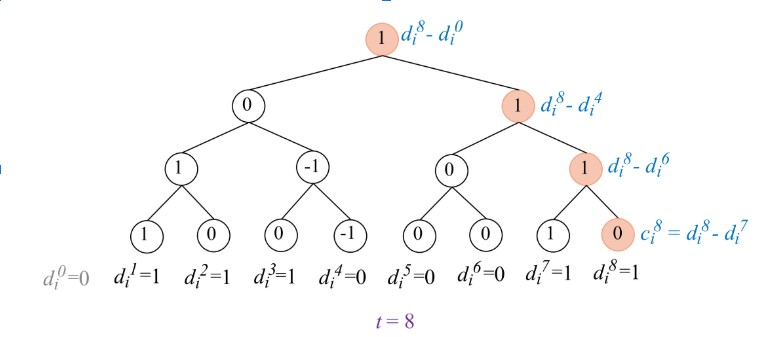
\includegraphics[width=0.9\textwidth]{figs/ddrm.jpg}
    \caption{تهیه‌ی درخت تفاوت از داده‌ها. برگرفته از \مرجع{Xue2023DDRMAC}}
    \label{fig:ddrmDifferenceTree}
\end{figure}

\فقره تصادفی‌سازی گره ارسالی

پس از انتخاب گره، باید به آن نوفه اضافه کنیم. با توجه به مقدار گره، طبق الگوریتم \رجوع{الگوریتم: سازوکار آشفته‌سازی گره ارسالی} عمل می‌کنیم. اگر مقدار گره 0 باشد (داده تغییر نکرده)، با احتمال برابر به 1+ یا 1- تبدیل می‌شود و هیچ بودجه حریم خصوصی مصرف نمی‌کند. اگر مقدار گره غیر 0 باشد (داده تغییر کرده)، با احتمال خاصی که حریم خصوصی تفاضلی را ارضا کند، مقدار 1+ یا 1- تنظیم می‌شود.  این فرآیند بخشی از بودجه حریم خصوصی کاربر را مصرف می‌کند.

\شروع{الگوریتم}{سازوکار آشفته‌سازی گره ارسالی}
\ورودی گره $v \in \{-1, 0, 1\}$ و بودجه‌ی حریم خصوصی $\epsilon$
\خروجی مقدار نوفه‌دار شده‌ی $\tilde{v}$

\If {$v = 0$}
    \دستور  $\tilde{v} = 
        \begin{cases} 
        \phantom{-}1, & \text{w.p. } \hspace{5pt} 0.5 \\
        -1, & \text{w.p. } \hspace{5pt} 0.5
        \end{cases}$
\Else
    \دستور $\tilde{v} = 
        \begin{cases} 
        \phantom{-}1, & \text{w.p. } \hspace{5pt} \frac{1}{2} + \frac{v}{2} \cdot \frac{e^{\epsilon}-1}{e^{\epsilon}+1} \\
        -1, & \text{w.p. } \hspace{5pt} \frac{1}{2} - \frac{v}{2} \cdot \frac{e^{\epsilon}-1}{e^{\epsilon}+1}
        \end{cases}$
\EndIf

\دستور $\tilde{v}$ را برگردان

\پایان{الگوریتم}

\فقره مدیریت بودجه حریم خصوصی

مقاله یک پارامتر به نام $k$ تعریف می‌کند. هر کاربر تنها $k$ بار مجاز است مقادیر غیرصفر را گزارش دهد. پس از آن، بودجه حریم خصوصی او تمام شده تلقی می‌شود و برای جلوگیری از نشت اطلاعات، همیشه مقادیر تصادفی ارسال می‌کند. همچنین روشی بهینه برای تعیین مقدار k ارائه می‌شود تا دقت کلی به حداکثر برسد.

\پایان{شمارش}


کارپذیر داده‌های تصادفی را از همه کاربران دریافت می‌کند. سپس با روش‌های آماری، سعی می‌کند نوفه را حذف کند. از آنجایی که در هر لحظه دو نوع گزارش دریافت شده (از گره‌های برگ و گره‌های ریشه)، جمع‌کننده این دو تخمین را با یک میانگین وزنی هوشمند ترکیب می‌کند تا به یک تخمین نهایی و دقیق‌تر از فرکانس داده‌ها برسد. شکل \رجوع{fig:ddrmOverview} به صورت خلاصه، عملکرد روش دی.دی.آر.اِم را به تصویر می‌کشد.


\begin{figure}[h]
    \centering
    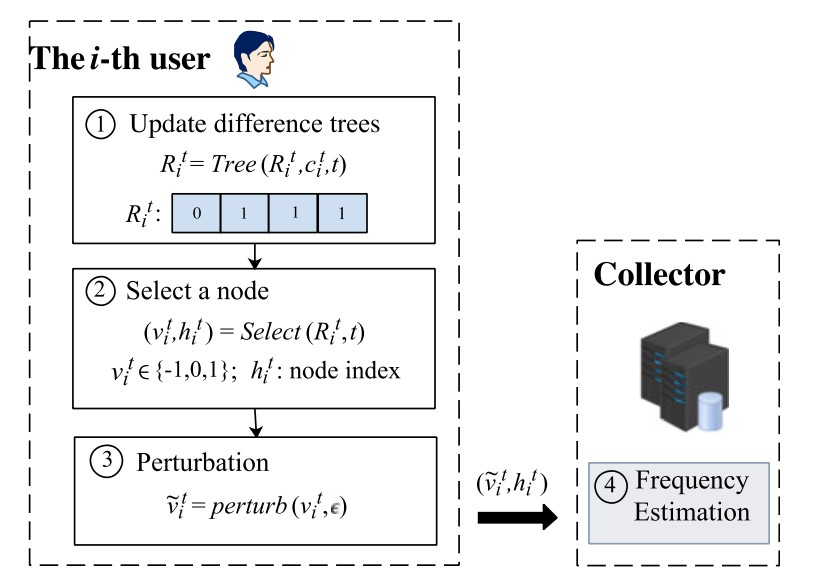
\includegraphics[width=0.9\textwidth]{figs/DDRM_overview.jpg}
    \caption{نحوه عملکرد روش دی.دی.آر.اِم. برگرفته از \مرجع{Xue2023DDRMAC}}
    \label{fig:ddrmOverview}
\end{figure}

درخت تفاوتی که این پژوهش ارائه می‌دهد مختص داده‌های دودویی است. با این حال مقاله راه حلی برای داده‌های غیر دودویی نیز بیان می‌کند. به این صورت که ورودی باید ابتدا با استفاده از کدگذاری یکانی به یک رشته دودویی تبدیل گردد. سپس برای هر بیت از این رشته، یک درخت تفاوت ساخته می‌شود.

روش دی.دی.آر.اِم با یک روش منحصر به فرد، مشکل داده‌های در حال تغییر را حل کرده است. ولی همچنان از معایب آن می‌توان به این مورد اشاره کرد که با افزایش دامنه‌ی داده‌ها، رسم درخت‌های تفاوت سربار زیادی سمت کاربر اعمال کرده و سودمندی نهایی کاهش پیدا می‌کند. 

\زیرقسمت{درهم‌سازی محلی}

درهم‌سازی، فرآیندی است که داده‌های ورودی با هر طولی را به یک خروجی با طول ثابت تبدیل می‌کند. این فرآیند چند ویژگی کلیدی دارد:

\شروع{فقرات}

\فقره یک‌طرفه بودن: از روی مقدار در‌هم‌سازی، نمی‌توان به داده اصلی دست یافت.

\فقره اثر بهمنی\پانویس{Avalanche Effect}: کوچکترین تغییری در داده ورودی، منجر به تغییری بزرگ و غیرقابل پیش‌بینی در خروجی می‌شود.

\فقره طول ثابت خروجی: صرف‌نظر از حجم داده ورودی، خروجی همواره طول ثابتی دارد.

\پایان{فقرات}

در روش درهم‌سازی محلی، هر کاربر قبل از ارسال داده خود، ابتدا آن را به صورت محلی درهم‌سازی می‌کند و سپس با استفاده از سازوکارهای حریم خصوصی تفاضلی محلی مانند پاسخ تصادفی، مقدار نتیجه را نوفه‌دار کرده و آن را برای کارپذیر ارسال می‌کند. درهم‌سازی محلی با ویژگی‌های ذاتی خود، راه‌حل‌های مؤثری برای این چالش‌ها ارائه می‌دهد:

\شروع{شمارش}

\فقره کارایی و کاهش سربار محاسباتی و ذخیره‌سازی

از آنجایی که خروجی تابع هش همواره طولی ثابت دارد، فرقی نمی‌کند که داده اصلی یک کاربر چقدر حجیم باشد؛ در نهایت یک مقدار با اندازه ثابت تولید می‌شود. این ویژگی به شدت حجم داده‌های ارسالی را کاهش داده و فرآیندهای محاسباتی و ذخیره‌سازی را در سمت سرور بهینه‌تر می‌کند.

\فقره مدیریت بهینه تغییرات در داده‌ها
 
هنگام وجود داده‌های پویا، اطلاعات یک کاربر ممکن است به طور مداوم تغییر کند. به لطف اثر بهمنی در توابع درهم‌ساز، هر تغییر جزئی در داده‌های کاربر، نتیجه‌ی کاملاً متفاوت ایجاد می‌کند. این ویژگی باعث می‌شود که سیستم بتواند به سرعت تغییرات را ثبت کند، بدون آنکه نیاز به مقایسه کامل داده‌های جدید و قدیم باشد.

\فقره افزایش حریم خصوصی در طول زمان

در داده‌های جریانی، یک مهاجم ممکن است تلاش کند با جمع‌آوری داده‌های یک فرد در طول زمان، به اطلاعات حساس او دست پیدا کند. از آنجایی که درهم‌سازی یک فرآیند یک‌طرفه است و با افزودن نوفه همراه می‌شود، حتی اگر مهاجم بتواند چندین داده تصادفی از یک کاربر را در طول زمان جمع‌آوری کند، بازسازی داده‌های اصلی یا مسیر تغییرات دقیق آنها عملاً غیرممکن خواهد بود.

\فقره سادگی در پیاده‌سازی و انطباق‌پذیری

الگوریتم‌های درهم‌ساز به طور گسترده‌ای در دسترس بوده و پیاده‌سازی آنها نسبتاً ساده است. این سادگی باعث می‌شود که بتوان به راحتی آنها را در سیستم‌های مختلف، از دستگاه‌های اینترنت اشیا با منابع محدود گرفته تا برنامه‌های کاربردی موبایل، به کار گرفت.

\پایان{شمارش}

در نتیجه، درهم‌سازی محلی با تبدیل داده‌های حجیم و متغیر به یک نمایش ثابت، فشرده و غیرقابل بازگشت، به یک ابزار قدرتمند در زرادخانه حریم خصوصی تفاضلی محلی تبدیل شده است. این روش نه تنها به حفظ حریم خصوصی کاربران در برابر جمع‌آورندگان داده کمک می‌کند، بلکه با بهینه‌سازی فرآیندها، تحلیل داده‌های پویا را در مقیاس بزرگ امکان‌پذیر می‌سازد.

\زیرزیرقسمت{پژوهش تیانهائو وانگ و همکاران}

پژوهش تیانهائو وانگ و همکاران \مرجع{Wang2017LocallyDP} یک کار تحقیقاتی مهم در زمینه حریم خصوصی تفاضلی است. این مقاله یک چارچوب کلی برای تحلیل و مقایسه پروتکل‌های مبتنی بر حریم خصوصی تفاضلی محلی معرفی می‌کند و سپس با استفاده از این چارچوب، پروتکل‌های موجود را بهینه‌سازی کرده و پروتکل‌های جدیدی ارائه می‌دهد.

مقاله نشان می‌دهد که پروتکل‌هایی مانند بازتاب ماتریس تصادفی\پانویس{Random Matrix Projection} در واقع یک نوع درهم‌سازی محلی دودویی\پانویس{Binary Local Hashing} هستند. در این روش، داده‌ی هر کاربر به یک بیت (۰ یا ۱) تبدیل می‌شود. این کار باعث از دست رفتن حجم زیادی از اطلاعات، حتی قبل از اضافه کردن نوفه برای حفظ حریم خصوصی می‌شود و دقت را کاهش می‌دهد.

محققان با شناسایی این ضعف، روشی به نام درهم‌سازی محلی بهینه\پانویس{Optimized Local Hashing} (به اختصار اُ.اِل.اِچ\پانویس{OLH}) را معرفی می‌کنند. ایده اصلی این است که به جای درهم‌سازی داده به یک بیت، آن را به دامنه‌ای بزرگتر با اندازه $g$ تبدیل می‌کنند. مهم‌ترین نوآوری مقاله این است که به صورت ریاضی ثابت می‌کند مقدار بهینه برای اندازه دامنه $g$ برابر با $e^\epsilon + 1$ است. با انتخاب این مقدار بهینه، به حداکثر دقت ممکن برای تخمین فرکانس دست می‌یابیم.

نتیجه نهایی، ارائه پروتکلی است که هم دقت بسیار بالایی دارد و هم هزینه ارتباطی بسیار پایینی در حد $O(\log n)$ دارد، که آن را برای کاربردهایی با مقادیر داده بسیار متنوع و زیاد، ایده‌آل می‌سازد. در مقاله، اثبات حفظ حریم خصوصی برای پروتکل عمومی درهم‌سازی محلی ارائه شده است. احتمال اینکه مقدار درهم‌سازی صحیح، به درستی گزارش شود را $p$ می‌نامیم. همچنین احتمال اینکه یک مقدار درهم‌سازی غلط، به اشتباه به جای مقدار صحیح گزارش شود را $q$ می‌نامیم.

این احتمالات را بر اساس بودجه حریم خصوصی و اندازه دامنه به شکل زیر تعریف می‌شوند:

$$p = \frac{e^\epsilon}{e^\epsilon + g - 1}$$
$$q = \frac{1}{e^\epsilon + g - 1}$$


برای اثبات حریم خصوصی، کافی است نشان دهیم که نسبت احتمال مشاهده خروجی برای هر دو ورودی دلخواه، از $e^\epsilon$ بیشتر نشود. این نسبت در بدترین حالت برابر با $\frac{p}{q}$ است.

\begin{equation}
\frac{p}{q} = \frac{ \frac{e^\epsilon}{e^\epsilon + g - 1} }{ \frac{1}{e^\epsilon + g - 1} } = e^\epsilon
\label{equ:worstCaseLDP}
\end{equation}

از آنجایی که این نسبت دقیقاً برابر با $e^\epsilon$ است، پروتکل تعریف‌شده، معیار حریم خصوصی تفاضلی محلی را برآورده می‌کند. یعنی حتی اگر مهاجم به خروجی دسترسی پیدا کند، اطلاعات بسیار محدودی درباره ورودی اصلی کاربر به دست می‌آورد.


\زیرقسمت{ترکیب حفظ کردن و درهم‌سازی محلی}

برای اینکه بتوانیم هم مزایای درهم‌سازی را داشته باشیم و هم مشکل پرسش‌های مکرر را حل کنیم، باید قبل از درهم‌سازی نتیجه را ذخیره کرده تا بعد‌تر از آن استفاده کنیم.

\زیرزیرقسمت{پژوهش آرکولزی و همکاران}

پژوهش آرکولزی و همکاران \مرجع{Arcolezi2022FrequencyEO} با معرفی یک پروتکل جدید به نام \مهم{لولوها}\پانویس{LOLOHA} حریم خصوصی را روی داده‌های در حال تغییر تضمین می‌کند. پروتکل‌های موجود مانند رپور گوگل یا دی.بیت.فلیپ.پی.اِم مایکروسافت، در مواجهه با داده‌هایی که مدام تغییر می‌کنند، با یک مشکل جدی روبرو هستند. عملکرد کلی در این پروتکل‌ها با افزایش دامنه مقادیر ورودی کاهش پیدا می‌کند. برای مثال، اگر بخواهیم آدرس وب‌سایت‌های بازدید شده را جمع‌آوری کنیم، مقدار دامنه یک عدد میلیونی خواهد بود و این باعث می‌شود حفظ حریم خصوصی در طولانی‌مدت تقریبا غیرممکن شود.

لولوها از نقاط قوت پروتکل‌های قبلی الهام گرفته اما ضعف بزرگ آن‌ها را برطرف می‌کند. عملکرد این پروتکل در سه قدم اصلی خلاصه می‌شود:

\شروع{شمارش}

\فقره کاهش دامنه

به جای کار با دامنه بزرگ $k$، هر کاربر قبل از هر کاری، داده واقعی خود را با استفاده از یک تابع درهم‌ساز، به یک عدد در یک دامنه بسیار کوچک‌تر به نام g تبدیل می‌کند. پس از این کار تعداد زیادی از مقادیر اصلی به یک مقدار یکسان نگاشت می‌شوند. بنابراین یک لایه ابهام و عدم قطعیت ایجاد می‌شود، زیرا کارپذیر حتی با داشتن نتیجه درهم‌سازی، مقدار واقعی را نمی‌داند.

\فقره تصادفی‌سازی و حفظ کردن نتیجه

پس از اینکه داده به یک مقدار در دامنه کوچک تبدیل شد، به آن نوفه اضافه کرده و نتیجه را در حافظه دستگاه ذخیره می‌کند. اگر در آینده داده کاربر تغییر کند اما مقدار درهم‌سازی آن همان مقدار قبلی باشد، پروتکل همان گزارش نوفه‌دار قبلی را دوباره ارسال می‌کند. این کار از هدر رفتن بودجه حریم خصوصی جلوگیری کرده و سرعت عملیات را بالا می‌برد.

به منظور آشفته‌سازی از سازوکار پاسخ تصادفی عمومی استفاده می‌شود. مقادیر $p$ و $q$ بر اساس قاعده‌ی \رجوع{equ:GRR} به صورت زیر مقداردهی می‌شوند. دقت کنید از $k$ به عنوان دامنه‌ی جدید استفاده شده است.

\begin{equation}
p = \frac{e^\epsilon}{e^\epsilon + k - 1}, \quad q = \frac{1-p}{k-1}
\label{equ:set-p-q}
\end{equation}

برای تخمین شمارش هر ورودی $v \in V$، تعداد باری که $v$ گزارش شده است را می‌شماریم (با نماد $C(v)$) و در فرمول زیر جایگزاری می‌کنیم:

\begin{equation}
\hat{f}(v) = \frac{C(v) - nq}{n(p - q)}
\end{equation}

در عبارت بالا، $n$ تعداد کاربران را نمایش می‌دهد. در پژوهش تیانهائو وانگ و همکاران \مرجع{Wang2017LocallyDP} اثبات می‌شود که ارزش مورد انتظار\پانویس{Expected Value} $\hat{f}(v)$ برابر با شمارش واقعی داده‌ها است.

$$E(\hat{f}(v)) = f(v)$$

\فقره تصادفی‌سازی دوباره

روش لولوها برای افزایش بیشتر امنیت و جلوگیری از حملات ردیابی، یک قدم دیگر نیز اضافه می‌کند. مانند رپور قبل از ارسال نهایی گزارش، یک لایه‌ی دیگر از نوفه به نتیجه مرحله قبل اضافه می‌کند. این کار باعث می‌شود حتی اگر مقدار درهم‌سازی کاربر تغییر کند، تشخیص این تغییر برای کارپذیر بسیار دشوار شود و حریم خصوصی کاربر در برابر تحلیل‌های زمانی محافظت شود.

تصادفی‌سازی مانند مرحله‌ی قبل انجام می‌شود. از آنجایی که دوبار از پاسخ تصادفی عمومی استفاده شده است، باید از عبارت زیر برای تخمین شمارش داده‌ها استفاده کنیم:

\begin{equation}
\hat{f}_L(v) = \frac{\frac{C(v) - nq_2}{(p_2 - q_2)} - nq_1}{n(p_1 - q_1)} = \frac{C(v) - nq_1(p_2 - q_2) - nq_2}{n(p_1 - q_1)(p_2 - q_2)}
\label{equ:estimateFrequency}
\end{equation}

در عبارت بالا، $p_1$ و $q_1$ ضرایب احتمالی تصادفی سازی اول، و $p_2$ و $q_2$ ضرایب احتمالی تصادفی‌سازی دوم هستند.

\پایان{شمارش}

این پژوهش دو پارامتر $\epsilon_1$ و $\epsilon_\infty$ را روی بودجه‌ی حریم خصوصی معرفی می‌کند. $\epsilon_\infty$ حد نهایی برداشت از بودجه‌ی حریم خصوصی شما برای یک داده خاص است. مهم نیست چند بار آن داده‌ را گزارش می‌کنید، کل هزینه حریم خصوصی که برای این داده می‌پردازید، هرگز از $\epsilon_\infty$  بیشتر نخواهد شد. این پارامتر به صورت مستقیم در تصادفی‌سازی دائمی (مرحله اول تصادفی سازی) استفاده می‌شود.

پارامتر $\epsilon_1$ هزینه اولین گزارش شما برای آن داده خاص است. این هزینه، میزان نشت اطلاعات در اولین باری که داده‌ را گزارش می‌دهید، مشخص می‌کند. از $\epsilon_1$ در محاسبه‌ی بودجه‌ی حریم خصوصی برای لایه دوم نوفه استفاده می‌شود. ما می‌خواهیم تضمین کنیم که حریم خصوصی کل برای یک گزارش واحد پس از دو مرحله تصادفی‌سازی، دقیقاً برابر با $\epsilon_1$ باشد.  پس باید بودجه‌ی حریم خصوصی تصادفی‌سازی آنی (مرحله دوم تصادفی سازی) را طوری تنظیم کنیم تا مجموع این دو لایه نوفه، ما را دقیقاً به $\epsilon_1$ برساند.


احتمال پاسخ نهایی صحیح به دو صورت ممکن است رخ دهد:

\شروع{فقرات}

\فقره سازوکار اول و دوم هر دو پاسخ درست را برگردانند.

$$p = p_1 \times p_2$$

\فقره سازوکار اول جواب غلط برگرداند ولی سازوکار دوم با تغییر پاسخ این اشتباه را جبران کند.

$$p = q_1 \times q_2$$
\پایان{فقرات}

پس احتمال کل پاسخ صحیح برابر است با:
$$p_{total} = (p_1 \times p_2) + (q_1 \times q_2)$$

احتمال پاسخ نهایی غلط نیز به دو صورت ممکن است رخ دهد:

\شروع{فقرات}

\فقره سازوکار اول جواب درست را برگردانده ولی سازوکار دوم پاسخ اشتباه را ارائه دهد.

$$q = p_1 \times q_2$$

\فقره سازوکار اول جواب غلط برگرداند و سازوکار با تغییر ندادن پاسخ، نتیجه را ثابت نگه دارد.

$$q = q_1 \times p_2$$
\پایان{فقرات}

پس احتمال کل پاسخ غلط برابر است با:
$$q_{total} = (p_1 \times q_2) + (q_1 \times p_2)$$

اکنون با توجه به عبارت \رجوع{equ:worstCaseLDP} می‌توان مقدار $\epsilon_1$ را محاسبه کرد:

$$\epsilon_1 = \ln \left( \frac{p_{total}}{q_{total}} \right) = \ln \left( \frac{p_1 p_2 + q_1 q_2}{p_1 q_2 + q_1 p_2} \right)$$

همچنین مقادیر $\epsilon_\infty$ و $\epsilon_{IRR}$ بر اساس عبارت \رجوع{equ:worstCaseLDP} به صورت زیر بدست می‌آیند:

$$\epsilon_\infty = \ln \left( \frac{p_1}{q_1} \right), \quad \epsilon_{IRR} = \ln \left( \frac{p_2}{q_2} \right)$$

اکنون با توجه به عبارات قبل، مقدار $\epsilon_{IRR}$ به صورت زیر بدست می‌آید:
$$\epsilon_{IRR} = \ln \left( \frac{e^{\epsilon_{\infty}+\epsilon_1} - 1}{e^{\epsilon_{\infty}} - e^{\epsilon_1}} \right)$$

الگوریتم \رجوع{الگوریتم: عملکرد لولوها سمت کاربر} نحوه‌ی عملکرد لولوها در سمت کاربر را نشان می‌دهد. این پژوهش دو رویکرد فراهم می‌کند تا مدیران سامانه بتوانند بر اساس نیاز خود بین حریم خصوصی و دقت، توازن برقرار کنند:

\شروع{فقرات}

\فقره لولوهای دودویی\پانویس{BiLOLOHA}: با انتخاب مقدار 2 برای $g$، می‌توان به قوی‌ترین سطح از حریم خصوصی طولی دست یافت که برای شرایط بسیار حساس ایده‌آل است.

\فقره لولوهای بهینه\پانویس{OLOLOHA}: پروتکل می‌تواند مقدار بهینه $g$ را برای به حداکثر رساندن دقت آماری پیدا کند، در حالی که همچنان هزینه حریم خصوصی بسیار پایین‌تر از پروتکل‌های دیگر باقی می‌ماند.

\پایان{فقرات}

\شروع{الگوریتم}{عملکرد لولوها سمت کاربر}
\ورودی مقادیر ورودی کاربر $[v_1, v_2, \ldots, v_\tau]$، توابع درهم‌ساز $\mathcal{H}$ و بودجه‌های حریم خصوصی $0 < \epsilon_1 < \epsilon_\infty$ 
\خروجی ارسال مقدار نوفه‌دار شده‌ی $x''_t$ به و تابع درهم‌سازی $H$ کارپذیر

\دستور انتخاب تابع $H$ از $\mathcal{H}$ به صورت تصادفی و ارسال به کارپذیر

\دستور $\epsilon_{IRR} = \ln \left( \frac{e^{\epsilon_{\infty}+\epsilon_1} - 1}{e^{\epsilon_{\infty}} - e^{\epsilon_1}} \right)$

\For{هر واحد زمانی $t \in [1..\tau]$}
    \دستور $x = H(v_t)$
    \If{$x$ حفظ نشده بود}
        \دستور $x' = M_{\text{GRR}}(x; \epsilon_\infty)$ \Comment{تصادفی‌سازی دائمی}
        \دستور حفظ کن مقدار $x'$ را برای $x$
    \Else
        \دستور بازسازی مقدار $x'$ برای $x$
    \EndIf
    \دستور $x''_t = M_{\text{GRR}}(x'; \epsilon_{IRR})$ \Comment{تصادفی‌سازی آنی}
    \دستور ارسال $x''_t$ 
\EndFor

\پایان{الگوریتم}

\زیرقسمت{سایر روش‌ها}

\زیرزیرقسمت{پژوهش سونر و همکاران}

پژوهش سونر و همکاران \مرجع{Aydin2024BayesianFE} یک چارچوب جدید و تطبیقی برای جمع‌آوری داده‌های حساس از کاربران با حفظ حریم خصوصی تفاضلی محلی ارائه می‌دهد. در اکثر روش‌های موجود برای آشفته‌سازی، پاسخ هر فرد از طریق انتخاب یک پاسخ تصادفی با افزودن نوفه همراه می‌شود. این پاسخ تصادفی از میان تمام گزینه‌های موجود انتخاب می‌شود.

این پژوهش، راهکار نوینی بر اساس پاسخ تصادفی به طور تصادفی محدود شده است، را ارائه می‌دهد.  سازوکار هوشمند و پویایی که به جای تصادفی‌سازی پاسخ از میان تمام گزینه‌ها، به شکل زیر عمل می‌کند:

\شروع{فقرات}

\فقره یادگیری از گذشته: الگوریتم با استفاده از داده‌هایی که تاکنون به صورت نوفه‌دار شده جمع‌آوری کرده است، یاد می‌گیرد که کدام پاسخ‌ها در کل جمعیت محتمل‌تر هستند.

\فقره محدود کردن گزینه‌ها: برای هر کاربر جدید، به جای در نظر گرفتن همه پاسخ‌های ممکن، الگوریتم یک زیرمجموعه کوچک از محتمل‌ترین گزینه‌ها را پیش‌بینی می‌کند.

\فقره تصادفی‌سازی هوشمند: سپس، فرآیند پاسخ تصادفی‌شده را فقط در داخل همین زیرمجموعه محدود و محتمل اجرا می‌کند.

\پایان{فقرات}

این الگوریتم به طور خاص برای مدیریت داده‌هایی که توزیع آن‌ها در طول زمان تغییر می‌کند، طراحی شده است. الگوریتم منتظر نمی‌ماند تا حجم زیادی از داده‌ها جمع‌آوری شود و بعد یک مدل ثابت بسازد. بلکه هر داده جدید را به محض دریافت، به صورت ترتیبی و لحظه به لحظه پردازش می‌کند. با دریافت پاسخ نوفه‌دار شده‌ی هر کاربر جدید، از روش‌های تخمین بیزی\پانویس{Bayesian Estimation} استفاده می‌کند تا مدل خود را کمی اصلاح و به‌روز کند. از این رو، بازتاب دقیق‌تری از وضعیت فعلی داده‌ها دارد. در نهایت چون فضای تصادفی‌سازی کوچک‌تر و مرتبط‌تر است، نوفه‌ی کمتری به داده‌ها اضافه می‌شود.

\زیرزیرقسمت{پژوهش یومین و همکاران}

پژوهش یومین و همکاران \مرجع{Zhang2024FederatedHH} یک راهکار جدید برای تحلیل داده‌های پرتکرار با حفظ حریم خصوصی تفاضلی محلی ارائه می‌دهد. به بیان دیگر سازوکار جدیدی به نام درخت پیشوندی هدف-تراز\پانویس{Target-Aligning Prefix Tree} برای شناسایی داده‌های پرتکرار، ارائه می‌شود. راهکار پیشنهادی این پژوهش دو رویکرد اصلی را معرفی می‌کند:

\شروع{فقرات}

\فقره رویکرد توسعه انطباقی: این روش به جای استفاده از یک رویکرد ثابت، به صورت هوشمند و با توجه به توزیع فراوانی داده‌ها، تصمیم می‌گیرد که کدام پیشوندها برای شناسایی موارد پرتکرار مناسب‌تر هستند. این کار به افزایش دقت و کاهش نوفه همراه است.

\فقره رویکرد هرس مبتنی بر اجماع\پانویس{Consensus-Based Pruning}: در این راهکار، از دانش قبلی که به صورت تصادفی از کاربران به دست آمده، برای حذف نامزدهای غیرضروری استفاده می‌شود.

\پایان{فقرات}

\زیرزیرقسمت{پژوهش ژِنگ و همکاران}

پژوهش ژِنگ و همکاران \مرجع{Liu2025LocallyDP}، یک راهکار نوآورانه به نام «پاسخ تصادفی مشترک» را برای بهبود فرآیندهای مبتنی بر حریم خصوصی تفاضلی محلی ارائه می‌دهد. در روش‌های قدیمی مانند پاسخ تصادفی، هر فرد به صورت مستقل داده‌های خود را قبل از ارسال، کمی تغییر می‌دهد تا حریم خصوصی‌اش حفظ شود. مشکل اصلی این است که هرچه سطح حفاظت از حریم خصوصی بالاتر باشد، دقت و کارایی داده‌های جمع‌آوری‌شده برای تحلیل آماری (مانند تخمین فراوانی) کاهش می‌یابد.

در راهکار پیشنهادی این پژوهش به جای اینکه هر فرد به تنهایی عمل کند، کاربران به صورت تصادفی به گروه‌های دونفره تقسیم می‌شوند. سپس، اعضای هر گروه داده‌های خود را به صورت هماهنگ و مشترک تغییر می‌دهند. نکته کلیدی این است که هویت اعضای هر گروه برای تحلیلگر داده مخفی باقی می‌ماند. در نهایت همان سطح از ضمانت حریم خصوصی را که روش‌های قدیمی داشتند، ارائه می‌کند، اما در عین حال، دقت تخمین فراوانی را بهبود می‌بخشد.

\زیرزیرقسمت{پژوهش یونفی لی و همکاران}

پژوهش یونفی لی و همکاران \مرجع{Li2024MultidomainsPL} مدلی جدید به نام «حریم خصوصی تفاضلی محلی شخصی‌سازی‌شده چند دامنه‌ای» را معرفی می‌کند. یکی از مشکلات روش‌های فعلی این است که در جمع‌آوری داده‌ها، نیازهای کاربران برای تجمیع اطلاعات در دامنه‌های مختلف داده و همچنین ترجیحات شخصی آن‌ها برای سطوح مختلف حریم خصوصی را نادیده می‌گیرند.

راهکار ارائه شده در این مدل به کاربران این امکان را می‌دهد که بر اساس ترجیحات شخصی خود، آزادانه هم دامنه داده و هم بودجه حریم خصوصی را انتخاب کنند. بنابراین کاربران می‌توانند با انتخاب دامنه‌های کوچک‌تر، از کاهش سودمندی ناشی از افزودن نوفه جلوگیری کنند. همچنین این مدل به نیازهای متنوع کاربران برای حفاظت از داده‌هایشان در سطوح مختلف پاسخ می‌دهد و به آن‌ها کنترل بیشتری بر روی حریم خصوصی خود می‌دهد.

\زیرزیرقسمت{پژوهش بو جیانگ و همکاران}

پژوهش بو جیانگ و همکاران \مرجع{Jiang2024WhenFE} یک راهکار جامع و چندوجهی برای جمع‌آوری و تحلیل داده‌ها با حفظ حریم خصوصی تفاضلی محلی ارائه می‌دهد. به طور خلاصه، راهکار این پژوهش در دو بخش اصلی قابل توضیح است:

\شروع{فقرات}

\فقره بهبود تخمین شمارش برای داده‌های شناخته‌شده: پژوهشگران یک سازوکار جدید و انعطاف‌پذیر را معرفی می‌کنند که در آن، روش‌های موجود را به طور قابل توجهی بهبود می‌یابند و تعادل بهتری میان سه عامل حریم خصوصی، دقت و هزینه ارتباطی برقرار می‌شود.

\فقره جمع‌آوری داده‌ها با دامنه‌ی ناشناخته: برای حل چالش جمع‌آوری داده‌هایی که از قبل مشخص نیستند (مانند کلمات جدید در یک زبان)، این پژوهش یک راهکار کاملاً نوآورانه ارائه می‌دهد. این راهکار از یک معماری پیشرفته مبتنی بر رمزنگاری، درهم‌سازی و تحلیل  استفاده می‌کند. داده‌های هر کاربر قبل از ارسال، روی دستگاه خود او رمزنگاری می‌شود. یک کارپذیر واسط، پیام‌های رمزنگاری‌شده از کاربران مختلف را با هم مخلوط می‌کند تا ارتباط بین کاربر و پیامش از بین برود. سپس کارپذیر دیگری، پیام‌های درهم‌شده را دریافت کرده و بدون اینکه به محتوای اصلی داده‌ها دسترسی داشته باشد، به فراوانی داده‌ها را محاسبه می‌کند.

\پایان{فقرات}


\زیرزیرقسمت{پژوهش ماریراس نتو و همکاران}

پژوهش ماریراس نتو و همکاران \مرجع{MarreirasNeto2024LocallyDP} به چگونگی حفظ حریم خصوصی کاربران حین تخمین شمارش داده‌های طولی می‌پردازد. این مقاله پروتکل جدیدی ارائه نمی‌دهد، بلکه به صورت جامع و روش‌مند، عملکرد ترکیبی از پروتکل‌های حریم خصوصی تفاضلی محلی برای داده‌های طولی ارزیابی می‌کند. هدف این است که مشخص شود کدام روش، بهترین سودمندی را ضمن حفظ حریم خصوصی ارائه می‌دهد. بر اساس تحلیل‌های انجام‌شده، بهینه شده‌ی روش‌های کدگذاری یکانی متقارن و لولوها به عنوان کارآمدترین پروتکل‌ها برای تخمین شمارش در داده‌های طولی شناسایی شدند.

\قسمت{نتیجه‌گیری}

با بررسی سازوکارهای مروبط به حل چالش داده‌های با ابعاد بالا، مشکلاتی یافت می‌شود:

\شروع{فقرات}

\فقره نمونه‌برداری: سازوکارهای مربوط به این روش با در نظر گرفتن بخشی از داده به عنوان نماینده‌ی کل داده، موجب کاهش دقت تحلیل‌های آماری می‌شوند. مخصوصا اگر حجم داده‌ی دریافتی از کاربران کم باشد، سودمندی به شدت کاهش میابد.

\فقره خوشه‌بندی: خوشه‌بندی به خودی خود روشی کارامد محسوب می‌شود. منتها برای بدست آوردن خوشه‌های مناسب، باید میزان وابستگی میان ابعاد داده مشخص گردد. طبیعتا سمت کاربر نمی‌توان این وابستگی‌ها را مشخص کرد، زیرا هم حجم داده سمت یک کاربر کم بوده و همچنین منابع محاسباتی محدودی خواهد داشت. پس کاربران باید داده‌ی خود را برای کارپذیر فرستاده و سپس کارپذیر همبستگی میان ابعاد را مشخص کند. اگر در همین ابتدا، کاربران داده‌ی خود را به صورت خام برای کارپذیر بفرستند، حریم خصوصی نقض می‌گردد. بنابراین باید به داده‌های خود نوفه اضافه کنند تا حریم خصوصی حفظ گردد. با اضافه کردن نوفه، دیگر نمی‌توان تخمین درستی از احتمال توزیع مشترک داده‌ها بدست آورد. درنتیجه خوشه‌بندی انجام شده توسط کارپذیر سالم نخواهد بود و سودمندی الگوریتم‌ها زیر سوال می‌رود.

\فقره یافتن میزان همبستگی با کمک داده‌های تاریخی یا دانش قبلی: به این نکته هم اشاره کردیم که نمی‌توان همیشه روی داشتن این اطلاعات حساب باز کرد و بنابراین نیازمند الگوریتم مطمئن‌تری هستیم.

\پایان{فقرات}

همچنین در حوزه‌ی داده‌های در حال تغییر، الگوریتم‌هایی مانند رپور و دی.دی.آر.اِم  کارایی خود را با افزایش دامنه ورودی از دست می‌دهند. در پژوهش آرکولزی و همکاران \مرجع{Arcolezi2022FrequencyEO} اثبات می‌شود که روش دی.بیت.فلیپ.پی.اِم با اینکه سودمندی مناسبی دارد، ولی در وضعیت‌هایی حریم خصوصی آن نقض می‌شود. 

با وجود مشکلات بالا، الگوریتم پی.پی.اِم.سی با استفاده از تبدیل هار و روش لولوها با کمک درهم‌سازی محلی توانسته‌اند توازن خوبی بین حریم خصوصی و سودمندی بدست آورند. بنابراین در فصل بعد راهکاری ارائه می‌دهیم که با ترکیب روش لولوها و تبدیل هار، حریم خصوصی داده‌های با ابعاد بالا و در حال تغییر را به صورت یکجا تضمین کند. 





\فصل{راهکار پیشنهادی}

راهکار پیشنهادی شامل ترکیب بهبود یافته‌ی روش پی.پی.اِم.سی و لولوها می‌شود. این راهکار به طور همزمان دو چالش اساسی در دنیای حریم خصوصی تفاضلی محلی برای داده‌های با ابعاد بالا و در حال تغییر را هدف قرار می‌دهد. در این فصل ابتدا کلیت ساختار الگوریتم و نحوه‌ی عملکرد آن در طول زمان شرح داده‌ می‌شود. سپس جزئیات پیاده‌سازی به تفصیل بیان خواهد شد، در نهایت نیز راهکار پیشنهادی حاضر مورد ارزیابی قرار خواهد گرفت.

\قسمت{بررسی چارچوب راهکار پیشنهادی}

به صورت خلاصه، با استفاده از تبدیل هار تمام داده‌ها به دو جزء میانگین و بردار ویژه تجزیه شده، در فرایند تصادفی‌سازی قرار گرفته و سمت کارپذیر ارسال می‌شوند. مسیر ذکر شده، \مهم{فرایند اصلی} راهکار پیشنهادی را بیان می‌کند. منتها قبل از شروع این فرایند، باید اعمال اضافه‌تری روی داده‌های در حال تغییر انجام داد تا بتوان آنها را وارد فرایند اصلی کرد. شکل \رجوع{fig:thesisClient} به طور کلی رفتار الگوریتم سمت کاربر را نشان می‌دهد.

\begin{figure}[h]
  \centering
  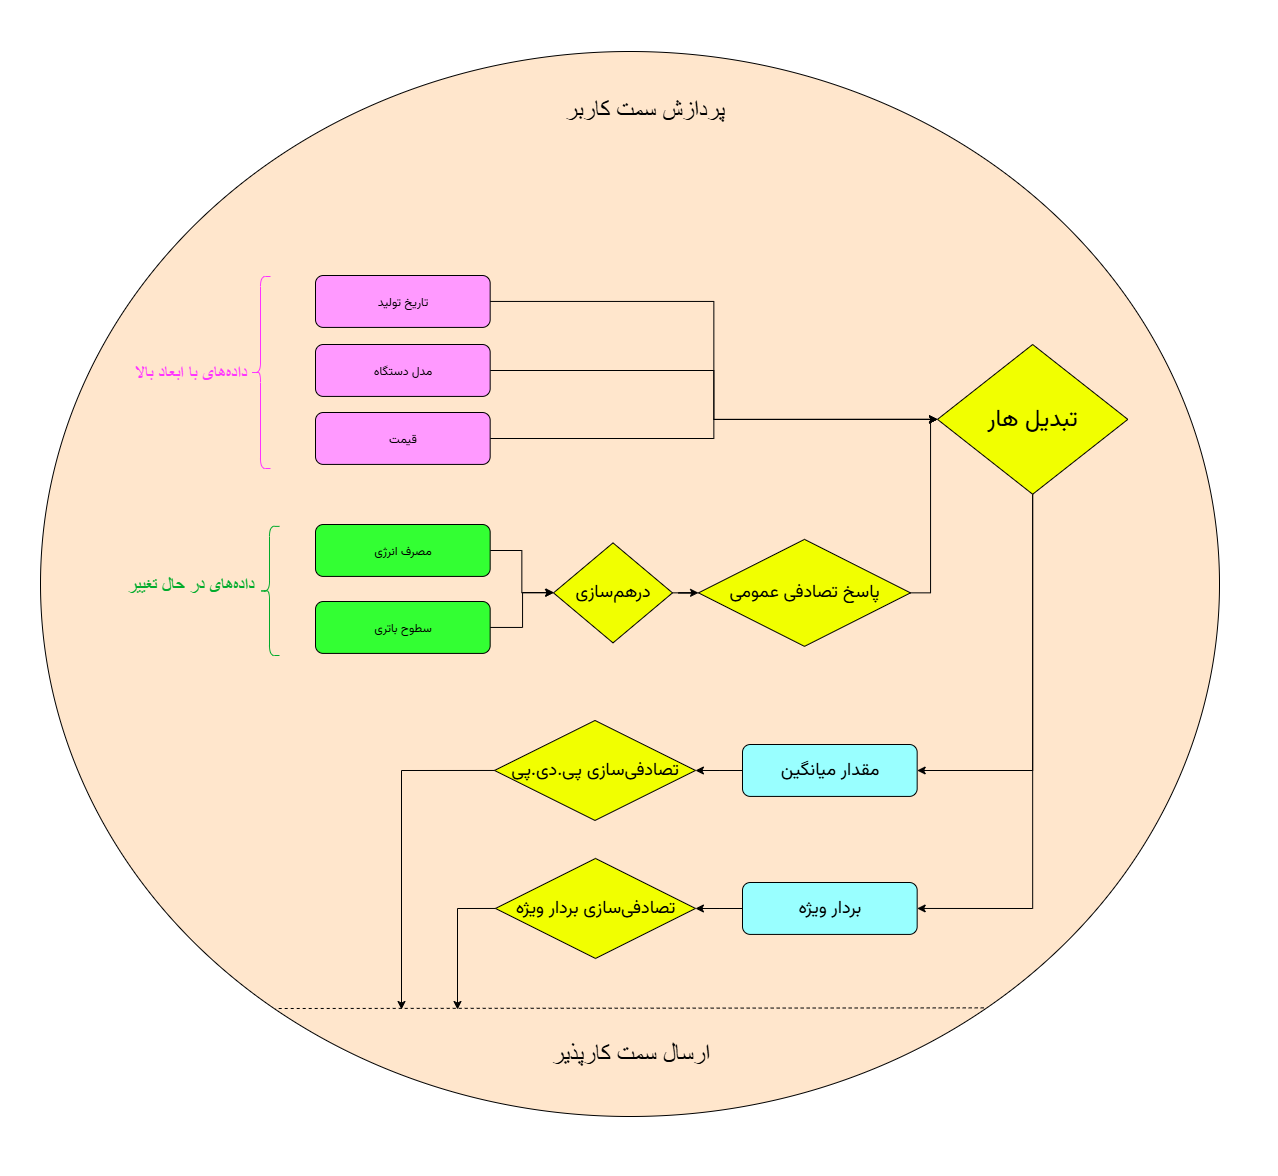
\includegraphics[width=0.9\textwidth]{figs/thesis-client.png}
  \caption{عملکرد روش پیشنهادی سمت کاربر}
  \label{fig:thesisClient}
\end{figure}


\زیرقسمت{فرایند مربوط به داده‌های در حال تغییر سمت کاربر}

پس از مشخص کردن داده‌های در حال تغییر، باید روش لولوها را روی این داده‌ها اعمال کنیم. هر کاربر یک تابع درهم‌ساز تصادفی انتخاب کرده و با استفاده از آن، دامنه‌ی داده‌ها را کاهش می‌دهد. درنتیجه چندین مقدار از دامنه اصلی به یک مقدار در دامنه کوچک نگاشت می‌شوند. این تصادم‌ها به صورت ذاتی یک لایه ابهام ایجاد می‌کنند که به حفظ حریم خصوصی کمک می‌کند. همچنین مطمئن می‌شویم که افزایش دامنه، تأثیر چندانی روی سودمندی نمی‌گذارد. سپس با کمک پاسخ تصادفی عمومی، شروع به آشفته‌سازی داده‌ها می‌کنیم. دقت کنید که این آشفته‌سازی از قوانین حفظ کردن پیروی می‌کند. الگوریتم \رجوع{الگوریتم: فرایند مربوط به یک بعد از داده‌های در حال تغییر سمت کاربر} این مرحله را به خوبی نمایش می‌دهد. 

در هنگام آشفته‌سازی مانند روش رپور از دو لایه تصافی‌سازی دائمی و آنی بهره گرفته و کاملا طبق الگوریتم \رجوع{الگوریتم: عملکرد لولوها سمت کاربر} پیاده‌سازی می‌شود. پس از این فرایند چند بعد از داده‌های ایمن ساخته‌ می‌شود و در کنار دیگر ابعاد ایستا به عنوان ورودی در فرایند اصلی قرار می‌گیرند.

\شروع{الگوریتم}{فرایند مربوط به یک بعد از داده‌های در حال تغییر سمت کاربر}
\ورودی مقادیر ورودی کاربر و متغیر در طول زمان $V = [v_1, v_2, \ldots, v_\tau]$ و بودجه‌های حریم خصوصی $\epsilon_\infty$ برای کل فرایند و $\epsilon_1$ برای تصادفی کردن یک گزارش واحد 
\خروجی بُعد نوفه‌دار شده با دامنه $g$

\دستور محاسبه‌ی اندازه دامنه‌ی جدید $g$ به صورت بهینه

\دستور انتخاب تابع درهم‌ساز $H$ به صورت تصادفی

\دستور کاهش دامنه: $hashed = H(V, g)$

\دستور تصادفی سازی: $perturbed = GRR(hashed, \epsilon_\infty, \epsilon_1)$

\دستور ارسال $perturbed$ سمت کارپذیر

\پایان{الگوریتم}

\زیرقسمت{فرایند اصلی مربوط به داده‌های با ابعاد بالا سمت کاربر}

ابتدا تمام داده‌ها باید در بازه‌‎ی $[-1, 1]$ یکنواخت\پانویس{Normalize} شوند. سپس با استفاده از تبدیل هار، داده‌های چند بعدی به دو مؤلفه مقدار میانگین و بردار ویژه تجزیه می‌شوند. مقدار میانگین با استفاده از روش پی.دی.پی نوفه‌دار می‌شود. به منظور تصادفی‌سازی بردار ویژه نیز از بهبودیافته‌ی الگوریتمی که در پی.پی.اِم.سی مطرح شد، استفاده ‌می‌کنیم. همچنین در هر دو تصادفی‌سازی از روش حفظ کردن بهره می‌گیریم تا هم در برابر پرسش‌های مکرر ایمن باشیم و هم سرعت عملیات را افزایش دهیم. در نهایت همگی داده‌ها برای کارپذیر ارسال می‌شوند. الگوریتم \رجوع{الگوریتم: فرایند اصلی مربوط به داده‌های با ابعاد بالا سمت کاربر} این مرحله را به صورت کلی نشان می‌دهد.

\شروع{الگوریتم}{فرایند اصلی مربوط به داده‌های با ابعاد بالا سمت کاربر}
\ورودی داده‌های با ابعاد بالا $A = [a_1, a_2, \ldots, a_d]$، دامنه تغییرات $domains$ و بودجه‌ی حریم خصوصی $\epsilon_\infty$
\خروجی میانگین و بردار ویژه به صورت نوفه‌دار شده

\دستور یکنواخت سازی در بازه‌ی $[-1, 1]$ : $normalized = normalize(A, domains)$

\دستور استخراج میانگین و بردار ویژه: $avg, eigenvector = HaarTransform(A)$

\دستور اضافه کردن نوفه به میانگین: $avg' = PDP(avg, \epsilon_\infty)$

\دستور اضافه کردن نوفه به بردار ویژه: $eigenvector' = improvedGPM(eigenvector, \epsilon_\infty)$

\دستور ارسال $avg'$ و $eigenvector'$ سمت کارپذیر

\پایان{الگوریتم}

\زیرقسمت{جمع‌آوری و تحلیل داده‌ها توسط کارپذیر}

کارپذیر پس از دریافت مقدار میانگین و بردار ویژه‌ی نوفه‌‌دار شده، معکوس تبدیل هار را اجرا کرده و داده‌هایی نزدیک به داده‌های اصلی را بدست می‌آورد. به منظور ارزیابی، روی داده‌های در حال تغییر تخمین شمارش صورت گرفته و روی دیگر ابعاد دو معیار احتمال توزیع داده‌ها و خطای مجذور میانگین\پانویس{Mean Square Error} اندازه‌گیری می‌شود.

از آنجایی که داده‌ها کاملا اعشاری هستند، باید ابتدا به نزدیک‌ترین مقدار صحیح رُند شده و سپس بر اساس روش تجمیع بیان‌شده در لولوها تخمین شمارش انجام شود. این اقدامات در الگوریتم فلان مشخص شده اند.


\شروع{الگوریتم}{جمع‌آوری و تحلیل داده‌ها توسط کارپذیر}
\ورودی میانگین $avg'$ و بردار ویژه $eigenvector'$ به صورت نوفه‌دار شده، تعداد ابعاد $d$ و دامنه تغییرات $domains$
\خروجی محاسبه‌ی تقریبی داده‌های اصلی به منظور انجام تحلیل آماری

\دستور بازگردانی ابعاد با کمک معکوس تبدیل هار: $\hat{D} = inverseHaar(avg', eigenvector', d)$

\دستور بازگردانی داده‌ها به بازه‌ی اصلی: $\hat{D} = denormalize(\hat{D}, domains)$

\دستور استفاده از $\hat{D}$ به منظور انجام تحلیل‌های آماری

\دستور جداسازی ابعاد در حال تغییر: $\hat{E} = \hat{D}\{d_i | d_i \hspace{5pt} \text{evolving is}\}$

\دستور رُند کردن به نزدیک‌ترین مقدار صحیح: $rounded = round(\hat{E})$

\دستور تخمین شمارش روی $\hat{E}$ با استفاده از فرمول \رجوع{equ:estimateFrequency}

\پایان{الگوریتم}

\قسمت{محاسبه‌ی اندازه دامنه‌ی جدید به صورت بهینه}

مقدار $g$ در پروتکل لولوها، اندازه دامنه جدید و کاهش‌یافته است که از طریق درهم‌سازی به دست می‌آید. انتخاب درست $g$ تعادل بین حریم خصوصی و سودمندی را برقرار می‌کند. با کاهش این مقدار ذکر شده، حریم خصوصی افزایش میابد ولی سودمندی افت خواهد کرد. از طرفی بزرگ بودن دامنه، باعث کاهش تصادم‌ها شده و در نتیجه، سودمندی افزایش میابد.

در آمار، سودمندی یا دقت یک تخمین‌گر، معمولاً به صورت معکوس با واریانس آن سنجیده می‌شود. واریانس بالا یعنی تخمین‌های ما پراکندگی زیادی حول مقدار واقعی دارند و غیرقابل اعتماد هستند. از طرفی واریانس پایین به این معناست که تخمین‌های ما به مقدار واقعی بسیار نزدیک هستند. بنابراین، هدف ما انتخاب یک $g$ مناسب است که به موجب آن، واریانس تخمین شمارش کمینه شود.


با توجه به فرمول \رجوع{equ:estimateFrequency} که تخمین شمارش بر اساس ورودی‌های پاسخ تصادفی عمومی را بیان می‌کند، می‌توان مقدار واریانس را به صورت تقریبی بدست آورد:

\begin{equation}
\mathbb{V}^*[\hat{f}_L(v)] = \frac{(p_2q_1 - q_2(q_1-1))(-p_2q_1 + q_2(q_1-1)+1)}{n(p_1-q_1)^2(p_2-q_2)^2}
\end{equation}

برای پیدا کردن نقطه‌ای که یک تابع در آن کمینه می‌شود، از مشتق استفاده می‌کنیم. پس از تابع واریانس نسبت به $g$ مشتق گرفته و برابر صفر قرار می‌دهیم تا نقاط بحرانی را پیدا کنیم.

$$\frac{\partial V^*(g)}{\partial g} = 0$$

با حل معادله‌ی بالا، مقدار بهینه‌ی $g$ را بدست می‌آوریم. برای ساده‌تر کردن نمایش فرمول نهایی، از دو متغیر کمکی استفاده شده است.

$$b = e^{\epsilon_\infty}, \quad a = e^{\epsilon_1}$$
\begin{equation}
g_{\text{optimal}} = 1 + \max\left(1, \left\lfloor \frac{1-a^2+\sqrt{a^4-14a^2+12ab(1-ab)+12a^3b+1}}{6(a-b)} \right\rfloor \right)
\end{equation}
\قسمت{درهم‌سازی}

برای پیاده‌سازی الگوریتم درهم‌سازی از کتابخانه‌ی ایکس.ایسک.هش\پانویس{xxhash} \مرجع{XxhashCitekeyMisc} در پایتون\پانویس{python} استفاده می‌کنیم. این کتابخانه از الگوریتمی استفاده می‌کند که سرعت بالایی داشته و عملکرد بهتری نسبت به الگوریتم‌هایی مانند اِم.دی.5\پانویس{MD5} و شا.وان\پانویس{SHA-1} دارد. این الگوریتم در مواردی مانند بررسی یکپارچگی داده‌ها، شناسایی فایل‌های تکراری و عملیات جستجو که سرعت در آنها اهمیت بالایی دارد، بسیار مناسب است.

قطعه کد \رجوع{code:xxhash} با استفاده از الگوریتم ایکس.ایسک.اچ.32\پانویس{xxh32}، هر یک از مقادیر موجود در ردیف داده‌های کاربر را به یک عدد صحیح درهم‌سازی کرده و سپس با استفاده از عملیات باقیمانده، آن را به یک محدوده مشخص نگاشت می‌دهد. این تابع یک مقدار اولیه $seed$ به عنوان ورودی درهم‌ساز دریافت می‌کند. مقدار اولیه برای هر کاربر به صورت تصادفی تولید می‌شود. در نتیجه ما از این عدد به عنوان تابع درهم‌ساز شخصی کاربران یاد می‌کنیم.

\LRE{
\begin{lstlisting}[language=Python, label=code:xxhash]
def reduce_domain_row(user_data_row, g, user_hash_function):
    return [
      (xxhash.xxh32(str(value), seed=user_hash_function).intdigest() % g)
      for value in user_data_row
    ]
\end{lstlisting}
}

\قسمت{یکنواخت‌سازی}

روش پی.پی.اِم.سی از تمام ابعاد میانگین گرفته و سمت کارپذیر می‌فرستد. در میانگین‌گیری اگر مقدار یک بُعد با اختلاف زیادی بیشتر از دیگر ابعاد باشد، نتیجه به سمت آن ویژگی سو می‌گیرد. پس قبل از تبدیل هار تمام ابعاد باید در یک بازه‌ی مشخص قرار گیرند. در روش پیشنهادی مانند الگوریتم پی.پی.اِم.سی تمام ابعاد در بازه‌ی $[-1, 1]$ یکنواخت می‌شوند.

این عملیات طبق کد \رجوع{code:normalization} با استفاده از روش مقیاس‌بندی کمینه-بیشینه\پانویس{Min-Max Normalization} پیاده‌سازی شده است.

\LRE{
\begin{lstlisting}[language=Python, label=code:normalization]
def normalize(x, domain):
    max_domain = max(domain)
    min_domain = min(domain)
    return ((2*(x-min_domain)) / (max_domain-min_domain)) - 1
\end{lstlisting}
}

\قسمت{بهبود روش جی.پی.اِم}

الگوریتم \رجوع{الگوریتم: سازوکار آشفته‌سازی بردار ویژه} روش جی.پی.اِم را به طور کامل توضیح داده است. خط 3 این الگوریتم تمام مقادیری از بردار ویژه که کمتر از حد آستاته هستند را صفر کرده و نوفه‌ای روی آنها اعمال نمی‌کند. از آنجایی که نوفه‌ی اضافی حذف شده است، سودمندی کمی بهبود یافته است ولی با صفر کردن این مقادیر، دقت نهایی به دشت افت خواهد کرد. فرض کنید تعداد زیادی از عناصر بردار ویژه مقداری کمتر از حد آستانه دارند؛ در این صورت تمام این عناصر مقدار صفر پیدا کرده و با انجام معکوس تبدیل هار، نتیجه اختلاف زیادی با مقدار اصلی پیدا می‌کند.

شاید با پیدا کردن حد آستانه مناسب بتوانیم مشکل ذکر شده را حل کنیم؛ ولی حد آستانه‌ی مناسب کاملا وابسته به داده‌ها و نوع اطلاعاتی است که کاربران ذخیره می‌کنند. اگر بخواهیم الگوریتم مستحکمی ارائه دهیم که با کمترین تغییر اکثر نیازمندی‌های ما را پوشش دهد، باید روش دیگری اتخاذ کنیم.

به منظور پیدا کردن راهکاری مناسب برای رسیدن به دقت بالاتر، کافیست این مقادیر کمتر از حد آستانه در همان مقدار خود باقی بمانند و فقط نوفه روی آنها اعمال نشود. نتایج ارزیابی روی چند مجموعه داده‌ی مختلف نشان داده است که این راهکار با حفظ حریم خصوصی تفاضلی، سودمندی بهتری خواهد داشت.

$$\tilde{e}_i = 
\begin{cases} 
e_i, & |e_i| \leq \theta \\
\text{from random at uniformly Sample} \hspace{5pt} [\frac{e_i \cdot e^{\epsilon}-1}{e^{\epsilon}-1}, \frac{e_i \cdot e^{\epsilon}+1}{e^{\epsilon}-1}], & v_i = 0 \\
\text{from random at uniformly Sample} \hspace{5pt} [-\frac{e^{\epsilon}+1}{e^{\epsilon}-1}, \frac{e_i \cdot e^{\epsilon}-1}{e^{\epsilon}-1}) \cup (\frac{e_i \cdot e^{\epsilon}+1}{e^{\epsilon}-1}, \frac{e^{\epsilon}+1}{e^{\epsilon}-1}], & v_i = 1 
\end{cases}$$


\قسمت{تضمین حریم خصوصی تفاضلی}

در این بخش به اثبات ریاضی امن بودن روش پیشنهادی می‌پردازیم. روش پیشنهادی از دو راهکار تبدیل هار و درهم‌سازی محلی استفاده شده است. در راهکار تبدیل هار، از دو سازوکار آشفته‌سازی پی.دی.پی و جی.پی.اِم استفاده می‌شود. در ادامه اثبات امن بودن این دو سازوکار بیان می‌شود.

\زیرقسمت{اثبات امن بودن سازوکار جی.پی.اِم}

سازوکار آشفته‌سازی سراسری برای حفاظت از حریم خصوصی بردار ویژه طراحی شده است. در این سازوکار، مجموعه‌ای شامل بردارهای دودویی به صورت تصادفی و مستقل از ورودی ساخته می‌شود. سپس به دو مجموعه‌ی $A$ و $B$ افراز خواهد شد. مجموعه‌ی $A$ شامل تمام بردارهایی است که تعداد اعضای 1 در آن‌ها زوج است. همچنین مجموعه‌ی $B$ شامل تمام بردارهایی است که تعداد اعضای 1 در آن‌ها فرد است. بر اساس قضیه‌ی دوجمله‌ای اندازه‌ی این دو مجموعه کاملا برابر خواهد بود. سپس یک متغیر تصادفی $X$ تعریف می‌شود که با احتمالی وابسته به $\epsilon$، یکی از دو مجموعه $A$ یا $B$ را انتخاب کرده و یک بردار به صورت تصادفی از مجموعه‌ی انتخاب شده استخراج می‌شود. در نهایت بر اساس بردار استخراج شده، بردار ویژه نوفه‌دار می‌شود.
 
برای اثبات باید نسبت احتمال تولید خروجی یکسان برای ورودی‌های متفاوت را بدست آوریم و نشان دهیم که این عدد کوچکتر یا مساوری $e ^ \epsilon$ خواهد بود. اکنون می‌خواهیم نسبت احتمال را برای یک خروجی دلخواه $y$ بررسی کنیم.

$$\Pr[X = 1] = \frac{e^{\varepsilon}}{e^{\varepsilon} + 1}
\quad
\Pr[X = 0] = \frac{1}{e^{\varepsilon} + 1}$$
$$
\Pr[y = v \mid V] =
\begin{cases}
\dfrac{e^{\varepsilon}}{e^{\varepsilon}+1} \cdot \dfrac{1}{|A|}, & v \in A, \\[10pt]
\dfrac{1}{e^{\varepsilon}+1} \cdot \dfrac{1}{|B|}, & v \in B .
\end{cases}$$

نسبت خروجی در بدترین حالت برای دو ورودی از دو مجموعه‌ی مختلف به صورت زیر بدست‌ می‌آید.
$$
\text{since } \hspace{5pt} |A| = |B|, \quad
\frac{\dfrac{e^{\varepsilon}}{e^{\varepsilon}+1}\cdot \dfrac{1}{|A|}}
     {\dfrac{1}{e^{\varepsilon}+1}\cdot \dfrac{1}{|B|}}
\;\;=\;\;
\frac{\dfrac{e^{\varepsilon}}{e^{\varepsilon}+1}}
     {\dfrac{1}{e^{\varepsilon}+1}}
\;\;=\;\; e^{\varepsilon}
$$

عبارت بالا نشان می‌دهد که مقدار بدست آمده همیشه کمتر از $e ^ \epsilon$ است. بنابراین سازوکار جی.پی.اِم به دلیل ساختار احتمالی و مستقل از ورودی خود، حریم خصوصی را تضمین می‌کند.

\زیرقسمت{اثبات امن بودن سازوکار پی.دی.پی}

سازوکار تصادفی یک مقدار آشفته‌شده را از یک توزیع احتمالی تولید می‌کند که شکل آن به ورودی الگوریتم بستگی دارد. توزیع احتمال به این صورت است که در ناحیه‌ی نزدیک به مقدار ورودی، احتمال انتخاب خروجی بیشتر از نواحی دیگر خواهد بود. برای اثبات $\epsilon{-}LDP$ بودن الگوریتم، باید نسبت تولید یک خروجی یکسان برای دو ورودی دلخواه را محاسبه کرده و بیشترین مقدار ممکن این نسبت را پیدا کنیم. بیشترین مقدار زمانی حاصل می‌شود که خروجی داخل بازه‌ی نزدیک به ورودی اول بوده و همچنین خارج از بازه‌ی نزدیک به ورودی دوم باشد: 


$$\frac{Pr[M(m_1) = y]}{Pr[M(m_2) = y]} = \frac{q.e^\epsilon}{q} = e^\epsilon$$


\زیرقسمت{اثبات امن بودن درهم‌سازی محلی}

در روش درهم‌سازی محلی از سازوکار تصادفی‌سازی عمومی برای نوفه‌دار کردن داده استفاده می‌شود. این سازوکار با توجه به مقادیر انتخابی $p$ و $q$، حریم خصوصی تفاضلی محلی را ارضا می‌کند. نحوه‌ی تنظیم این مقادیر در توضیح روش لولوها \رجوع{equ:set-p-q} به تفصیل بیان شده است.

\زیرقسمت{نتیجه‌گیری}

نشان دادیم که سازوکارهای مذکور همگی حریم خصوصی تفاضلی محلی را ارضا می‌کنند. روی داده‌های غیر پویا تنها سازوکارهای جی.پی.اِم و پی.دی.پی اجرا می‌شوند. پس با توجه به امن بودن چنین سازوکارهایی، می‌توان گفت حریم خصوصی برای داده‌های غیر پویا تضمین می‌شود. از طرفی روی داده‌های در حال تغییر هر سه سازوکار جی.پی.اِم، پی.دی.پی و تصادفی‌سازی عمومی به صورت متوالی انجام می‌شوند. این عملیات شامل قانون ترکیب متوالی نخواهد شد؛ زیرا ورودی سازوکارهای جی.پی.اِم و پی.دی.پی، خروجی سازوکار تصادفی‌سازی عمومی هستند و نمی‌‌توان گفت هر سه سازوکار روی یک داده‌ی ورودی اجرا می‌شوند. بنابراین می‌توان نتیجه گرفت راهکار پیشنهادی با موفقیت حریم خصوصی تفاضلی محلی را ارضا می‌کند.









\فصل{ارزیابی روش پیشنهادی}

در این فصل به ارزیابی روش پیشنهادی و مقایسه‌ی آن با چهار روش پی.اِم، دوچی، رپور و دی.بیت.فلیپ.پی.اِم می‌پردازیم. معیارهای خطای مجذور میانگین و اختلاف احتمال توزیع داده‌ها برای داده‌های با ابعاد بالا (روش‌های پی.اِم و دوچی) در نظر گرفته شده است. همچنین تخمین شمارش داده‌ها در مقایسه با پژوهش‌های مربوط به داده‌های در حال تغییر (روش‌های رپور و دی.بیت.فلیپ.پی.اِم) بررسی می‌شود. 

در این بخش ابتدا مجموعه داده ورودی معرفی شده و سپس نتایج ارزیابی روی دو دسته‌ی مذکور از داده‌ها بیان می‌شود. لازم به ذکر است که روش پیشنهادی همواره روی مجموعه‌ای از داده‌ها اجرا شده است که هم دارای ابعاد بالا بوده و هم به صورت مکرر تغییر می‌کنند. نتایج نشان می‌دهد که روش پیشنهادی با حفظ حریم خصوصی تفاضلی محلی، کارایی بهتری نسبت به الگوریتم‌های پیشین دارد.

\قسمت{مجموعه داده‌ی ورودی}

 به منظور ارزیابی راهکار پیشنهادی از مجموعه داده‌ی بزرگسالان\پانویس{Adult} استفاده شده است. این پایگاه داده از سرشماری سال ۱۹۹۴ ایالات متحده استخراج شده و یکی از معروف‌ترین مجموعه داده‌ها در حوزه یادگیری ماشین برای کارهای طبقه‌بندی است.

داده‌ها از نوع اعداد صحیح بوده و شامل اطلاعات شخصی و جمعیت‌شناختی افراد است. در این مجموعه داده ویژگی‌هایی مانند سن، سطح تحصیلات، وضعیت تاهل، نژاد و جنسیت وجود دارد. 15 ویژگی و 45222 رکورد از کاربران در این مجموعه داده گنجاده شده است و برای تست عملکرد الگوریتم روی داده‌های غیر دودویی و عددی که دارای همبستگی‌های پیچیده بین ویژگی‌های مختلف هستند، بسیار مفید است.

به منظور ارزیابی عملکرد راهکار پیشنهادی روی داده‌های در حال تغییر، از مجموعه‌ داده‌ی گردآوری شده در پژوهش لولوها استفاده شده است. نویسندگان این پژوهش یک مجموعه داده‌ی مصنوعی به اسم «سین\پانویس{Syn}» تهیه کرده اند. این مجموعه داده برای شبیه‌سازی دنیای واقعی طراحی شده است که در آن، داده‌ها به صورت دوره‌ای و مکرر (هر 6 ساعت یکبار) جمع‌آوری شده اند.

اندازه دامنه ۳۶۰ است که در واقع همان تعداد دقایق در یک بازه ۶ ساعته است. مجموعه داده سین از 10000 کاربر به تعداد 120 بار جمع‌آوری شده است. نحوه ساخت این داده‌ها طوری است که به خوبی وضعیت داده‌های در حال تغییر را شبیه سازی می‌کند.

به منظور ساخت مجموعه داده‌ای که هر دو ویژگی مطرح را داشته باشد باید دو مجموعه داده‌ی ذکر شده را با یکدیگر ترکیب کنیم. مطابق شکل \رجوع{fig:dataset} مجموع داده‌ی سین به صورت یک بُعد در کنار 15 بُعد مجموعه داده بزرگسالان قرار می‌گیرد.

\begin{figure}[h]
  \centering
  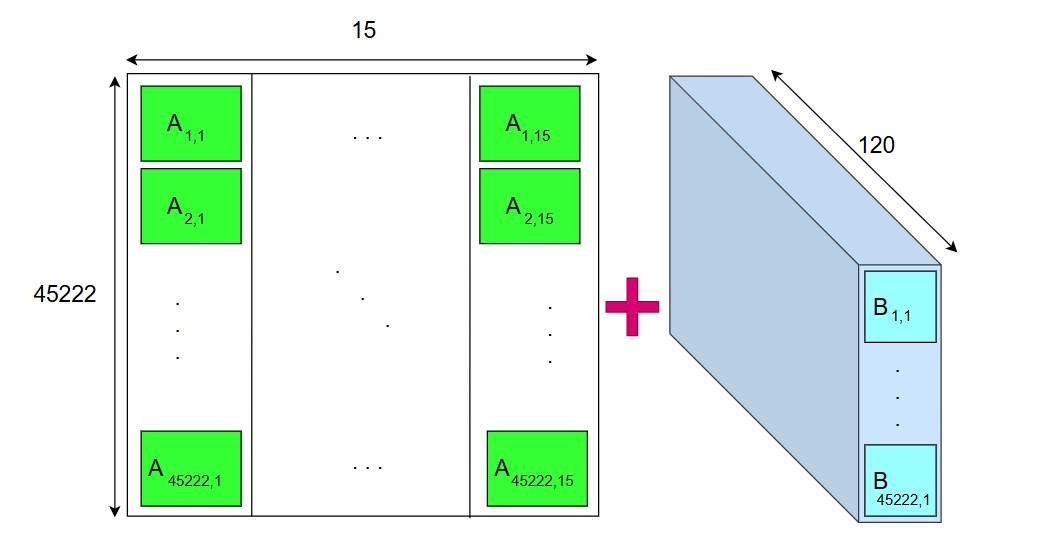
\includegraphics[width=0.9\textwidth]{figs/dataset.jpg}
  \caption{نحوه ترکیب دو مجموعه داده‌ی بزرگسالان و سین. مشخصه‌ی $A_{i,j}$ نشان دهنده‌ی ویژگی $j$ام از کاربر $i$ام است. همچنین نشان $B_{i,t}$، داده‌ی پویای کاربر $i$ام در واحد زمانی $t$ام را نمایش می‌دهد.}
  \label{fig:dataset}
\end{figure}

\قسمت{ارزیابی روی داده‌های با ابعاد بالا}

در این بخش معیار میانگین مربعات خطا و میانگین اختلاف توزیع احتمال داده‌ها با دو روش پی.اِم و دوچی مقایسه می‌شود.

\زیرقسمت{ارزیابی حین تغییر بودجه‌ی حریم خصوصی}

نمودار \رجوع{fig:eps_mse}، میانگین مربعات خطا را برای سه روش مختلف حفظ حریم خصوصی در برابر بودجه‌ی حریم خصوصی مقایسه می‌کند. محور عمودی نشان‌دهنده خطای روش و محور افقی، میزان بودجه حریم خصوصی است؛ هرچه $\epsilon$ بزرگ‌تر باشد، سطح حریم خصوصی کمتر و دقت مورد انتظار بالاتر است.

همانطور که در نمودار مشخص است، روش پیشنهادی (خط آبی) در تمام نقاط، به طور مداوم کمترین میزان خطا را نسبت به دو روش دیگر، یعنی روش پی.اِم و روش دوچی، به ثبت رسانده است. این موضوع بیانگر عملکرد برتر و دقت بالاتر الگوریتم ارائه‌شده است. روش دوچی در مقادیر پایین $\epsilon$، خطای بسیار بالایی دارد که با افزایش $\epsilon$ به سرعت کاهش می‌یابد اما همچنان بالاتر از دو روش دیگر باقی می‌ماند. روش پی.اِم عملکرد بهتری نسبت به روش دوچی دارد اما کماکان خطای آن به مراتب بیشتر از روش پیشنهادی ما است. این نتایج به وضوح نشان می‌دهد که الگوریتم جدید توانسته است مصالحه بهتری میان حفظ حریم خصوصی و دقت نتایج برقرار کند و کارایی بالاتری در تحلیل داده‌ها داشته باشد.

\begin{figure}[h]
  \centering
  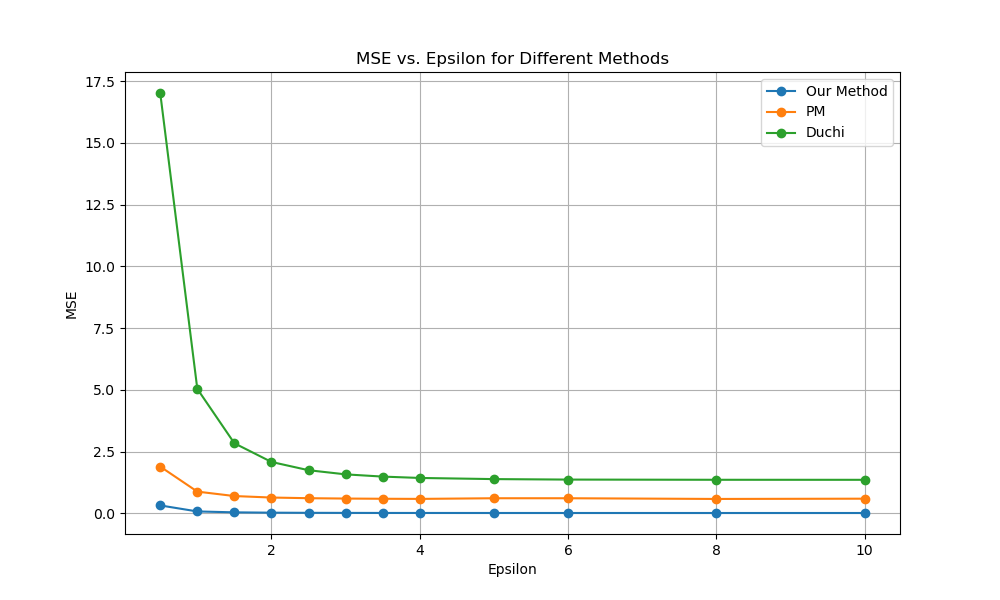
\includegraphics[width=0.9\textwidth]{figs/evaluation_eps_mse.png}
  \caption{مقایسه‌ی میانگین مربعات خطای روش پیشنهادی با دو روش پی.اِم و دوچی}
  \label{fig:eps_mse}
\end{figure}

همچنین نمودار \رجوع{fig:eps_avg}، میانگین اختلاف توزیع احتمال را برای سه روش مختلف و در سطوح بودجه‌ی حریم خصوصی، به تصویر می‌کشد. معیار میانگین اختلاف توزیع احتمال نشان می‌دهد که توزیع داده‌های نوفه‌دار شده تا چه حد به توزیع داده‌های اصلی شباهت دارد و مقدار کمتر آن، به معنای عملکرد بهتر است.

روش پیشنهادی (خط آبی)، پایداری مطلوبی داشته و در تقریباً تمام بازه $\epsilon$، کمترین میزان اختلاف را با توزیع اصلی داده‌ها نشان می‌دهد. این موضوع حاکی از توانایی بالای این روش در حفظ ساختار آماری و ویژگی‌های بنیادین داده‌هاست. در مقابل، روش دوچی (خط سبز) نه تنها در اکثر محدوده‌ها بیشترین میزان اختلاف را دارد، بلکه در مقادیر پایین $\epsilon$ رفتاری نامنظم و غیریکنواخت از خود بروز می‌دهد. این نوسان شدید، که احتمالاً ناشی از ماهیت تصادفی برخی عملیات‌های به کار رفته در این الگوریتم است، قابلیت اطمینان آن را کاهش می‌دهد. روش پی.اِم اگرچه از روش دوچی بهتر عمل می‌کند، اما همچنان با اختلاف قابل توجهی ضعیف‌تر از روش پیشنهادی ظاهر شده است. در نتیجه، می‌توان گفت الگوریتم ارائه شده در شرایطی که بودجه‌ی حریم خصوصی محدودی داریم، راهکاری بسیار دقیق‌تر و پایدارتر برای حفظ توزیع اصلی داده‌ها است.

\begin{figure}[h]
  \centering
  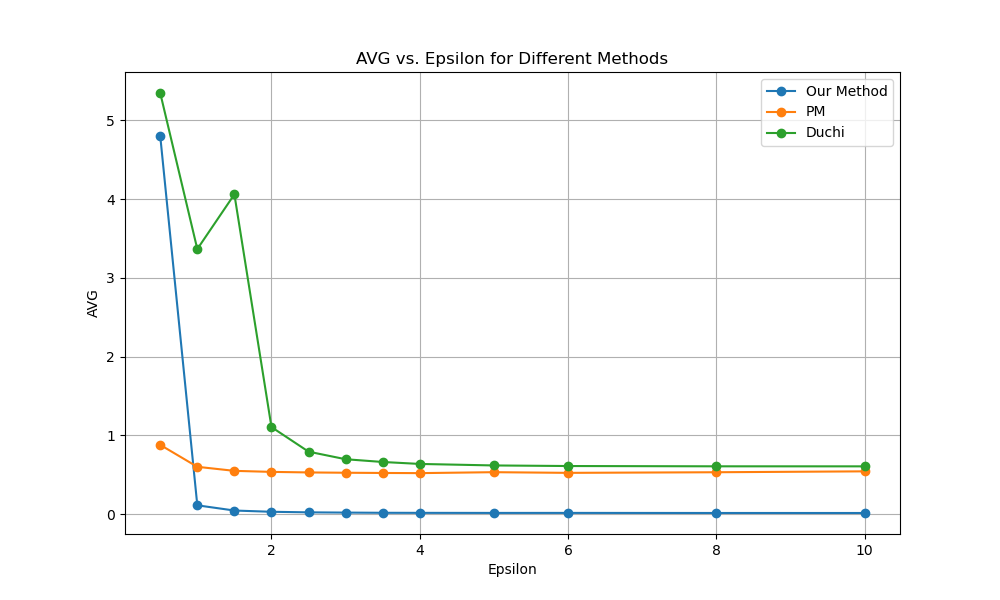
\includegraphics[width=0.9\textwidth]{figs/evaluation_eps_avg.png}
  \caption{مقایسه‌ی میانگین اختلاف توزیع احتمال داده‌ها در روش پیشنهادی با دو روش پی.اِم و دوچی}
  \label{fig:eps_avg}
\end{figure}

\زیرقسمت{ارزیابی حین تغییر تعداد ابعاد داده}

نمودار \رجوع{fig:dim_avg}، عملکرد سه روش مختلف را در مواجهه با افزایش تعداد ابعاد داده‌ها ارزیابی می‌کند. محور افقی نشان‌دهنده تعداد ابعاد و محور عمودی، میانگین خطای هر روش است. در تحلیل داده‌های پیچیده، پایداری یک الگوریتم در برابر افزایش ابعاد، یک شاخص کلیدی برای سنجش کارایی آن محسوب می‌شود.

روش پیشنهادی (خط آبی) برتری مطلق خود را به نمایش می‌گذارد. این روش در تمام طول بازه، با حفظ میانگین خطا در سطحی بسیار پایین و نزدیک به صفر، عملکردی بسیار پایدار از خود نشان می‌دهد. این ثبات، یک مزیت کلیدی است، زیرا نشان می‌دهد که با پیچیده‌تر شدن داده‌ها و افزایش ابعاد، کارایی الگوریتم کاهش پیدا نمی‌کند. روش پی.اِم (خط نارنجی) اگرچه از پایداری نسبی برخوردار است، اما سطح خطای آن به مراتب بالاتر از روش ما باقی می‌ماند. در مقابل، روش دوچی (خط سبز) نه تنها با اختلاف زیادی بیشترین خطا را دارد، بلکه با افزایش ابعاد، رفتاری نامنظم و غیرقابل پیش‌بینی از خود نشان می‌دهد. این نوسانات شدید بیانگر آن است که این روش به شدت به تغییرات در تعداد ابعاد حساس است و قابلیت اطمینان پایینی دارد.

\begin{figure}[h]
  \centering
  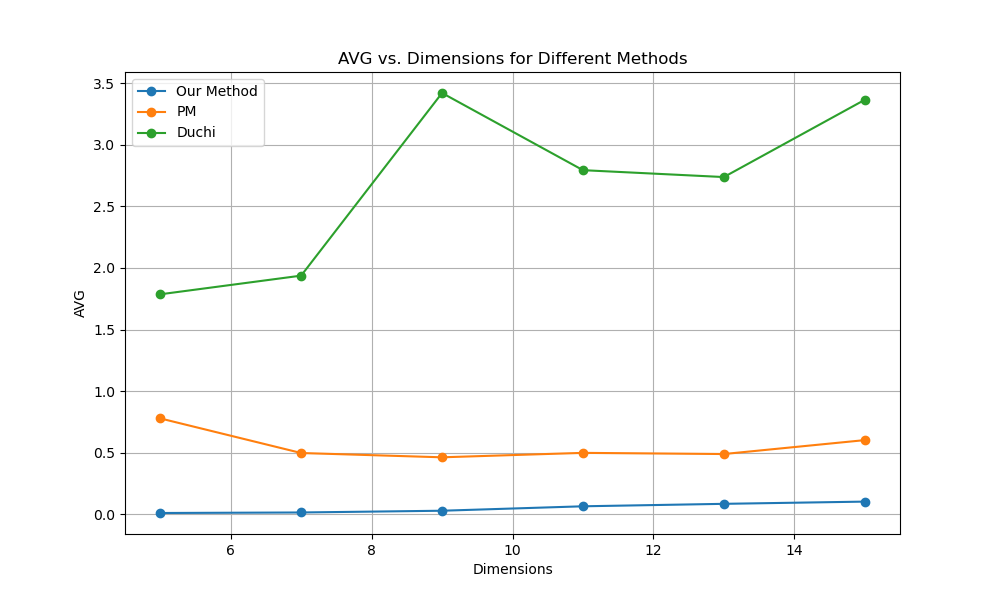
\includegraphics[width=0.9\textwidth]{figs/evaluation_dim_avg.png}
  \caption{مقایسه‌ی خطا در روش پیشنهادی حین تغییر تعداد ابعاد با دو روش پی.اِم و دوچی}
  \label{fig:dim_avg}
\end{figure}

\زیرقسمت{ارزیابی روی مجموعه داده‌های مختلف}

نمودار \رجوع{fig:dst_mse}، به ارزیابی عملکرد و قابلیت تعمیم‌پذیری سه روش مختلف در مواجهه با مجموعه داده‌های گوناگون می‌پردازد. روی محور افقی، برای هر مجموعه داده‌ی ورودی یک عدد تخصیص داده شده است و محور عمودی، میانگین مربعات خطا را نشان می‌دهد که مقدار کمتر آن، نشان‌دهنده دقت بالاتر است. بعضی از مجموعه داده‌ها نیز شامل مقادیر دودویی هستند.

روش پیشنهادی به‌طور پیوسته، کمترین میزان خطا را در تمامی مجموعه داده‌ها به ثبت رسانده است. این پایداری و دقت بالا نشان می‌دهد که الگوریتم ما از قابلیت تعمیم‌پذیری بسیار خوبی برخوردار است و عملکرد آن وابسته به نوع خاصی از توزیع داده نیست. در برخی نقاط، روند تغییرات خطا در روش پیشنهادی و روش پی.اِم شباهت‌هایی دارد؛ برای مثال، بین مجموعه‌ داده‌های شماره ۱۰ تا ۱۱، هر دو روش شاهد کاهش خطا بوده‌اند. این شباهت عملکرد در نمودار \رجوع{fig:dst_avg} که خطای احتمال توزیع مشرک داده‌ها را می‌سنجد، بیشتر به چشم می‌خورد.

\begin{figure}[h]
  \centering
  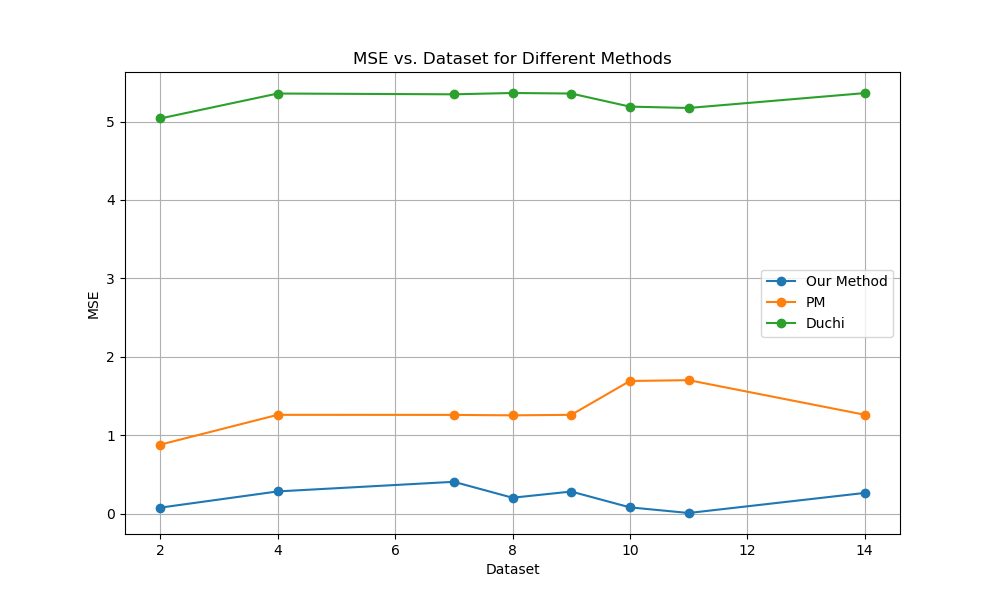
\includegraphics[width=0.9\textwidth]{figs/evaluation_dst_mse.png}
  \caption{مقایسه‌ی میانگین مربعات خطا در روش پیشنهادی حین تغییر مجموعه داده ورودی}
  \label{fig:dst_mse}
\end{figure}

\vspace{5pt}

\begin{figure}[h]
  \centering
  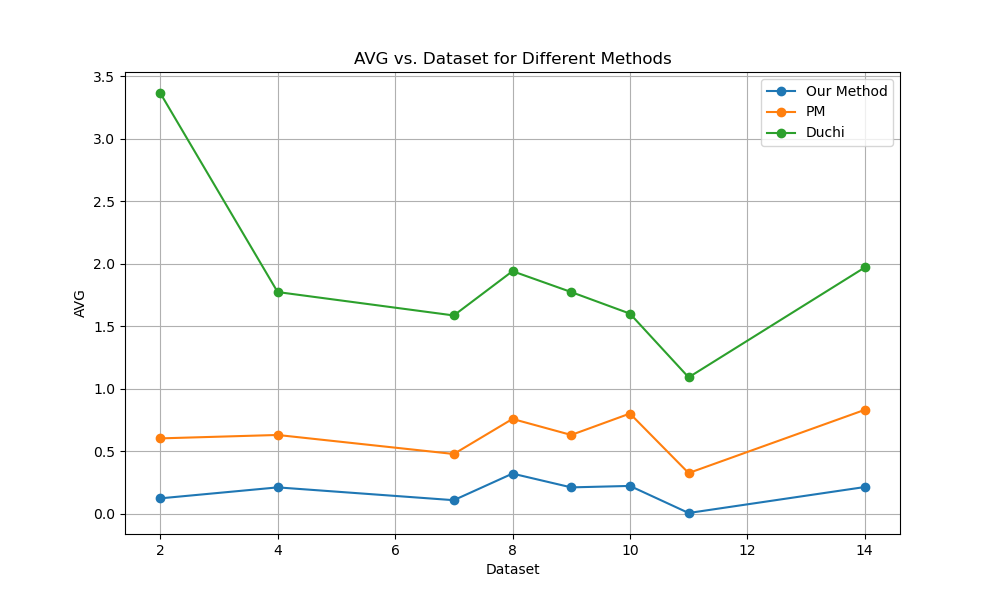
\includegraphics[width=0.9\textwidth]{figs/evaluation_dst_avg.png}
  \caption{مقایسه‌ی میانگین اختلاف توزیع احتمال داده‌ها حین تغییر مجموعه داده ورودی}
  \label{fig:dst_avg}
\end{figure}

\قسمت{ارزیابی روی داده‌های در حال تغییر}

محور عمودی نمودار \رجوع{fig:eps_frq} میانگین خطای تخمین شمارش را نشان داده و محور افقی نمایانگر تغییر بودجه‌ی حریم خصوصی است. الگوریتم پیشنهادی از نظر دقت، در سطحی کاملاً رقابتی و با فاصله‌ای ناچیز از دو روش رپور و دی.بیت.فلیپ.پی.اِم قرار دارد. در واقع بهبودهایی که روی حفظ حریم خصوصی داده‌های با ابعاد بالا انجام شده است، کمی دقت و سودمندی را کاهش داده است.

\begin{figure}[h]
  \centering
  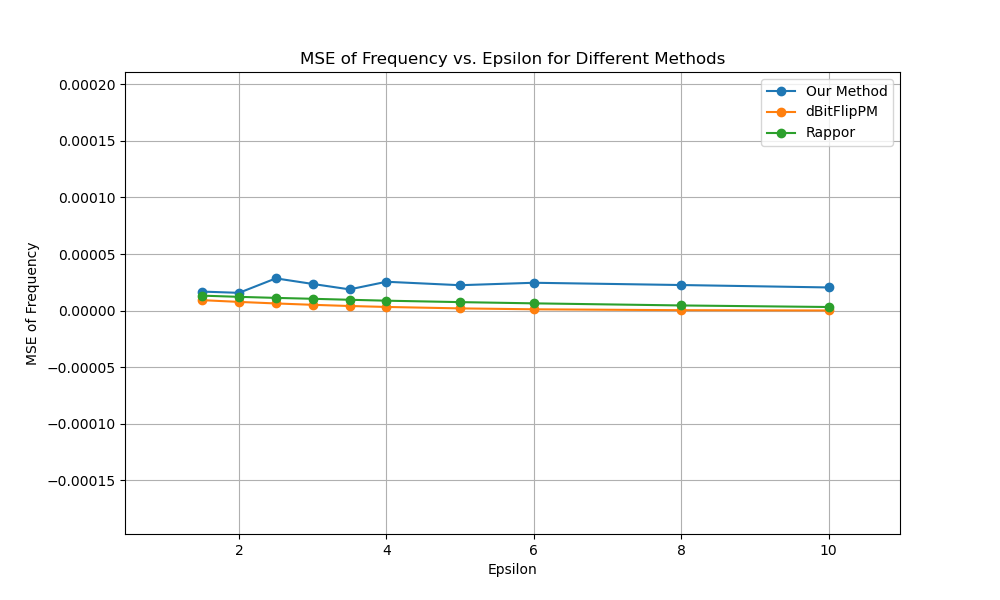
\includegraphics[width=0.9\textwidth]{figs/evaluation_eps_frq.png}
  \caption{مقایسه‌ی میانگین خطای تخمین شمارش در روش پیشنهادی حین تغییر بودجه‌ی حریم خصوصی}
  \label{fig:eps_frq}
\end{figure}

البته همانطور که در نموارد \رجوع{fig:usr_tim} مشاهده می‌کنید، با افزایش تعداد کاربران، زمان اجرای الگوریتم دی.بیت.فلیپ.پی.ام به صورت قابل توجهی افزایش می‌یابد. در مقابل، روش پیشنهادی با یک شیب بسیار ملایم‌تر، بهینگی مطلوبی را در مقیاس‌های بزرگ به نمایش می‌گذارد. این برتری در زمان اجرا، الگوریتم ما را به گزینه‌ای بسیار کارآمدتر برای پیاده‌سازی در سیستم‌های واقعی با میلیون‌ها کاربر تبدیل می‌کند. این مورد هم باید در نظر گرفت که الگوریتم رپور، با وجود خطای کمتر و سرعت بیشتر، دارای یک ضعف ذاتی در مواجهه با داده‌های در حال تغییر است. همانطور که قبل‌تر گفته شد، رپور در مواجه با داده‌هایی که به صورت مکرر تغییر می‌کنند ضعف داشته و به ازای هر تغییر کوچک، باید مقدار جدیدی حفظ کند. این فرایند روش حفظ کردن را زیر سوال برده و باعث نقض حریم خصوصی می‌شود. الگوریتم پیشنهادی این چالش کلیدی را به طور مستقیم هدف قرار داده و با ارائه‌ی یک سازوکار مقاوم، تضمین می‌کند که حریم خصوصی تفاضلی محلی حتی در صورت تغییر مداوم داده‌ها نیز به قوت خود باقی بماند.

\begin{figure}[h]
  \centering
  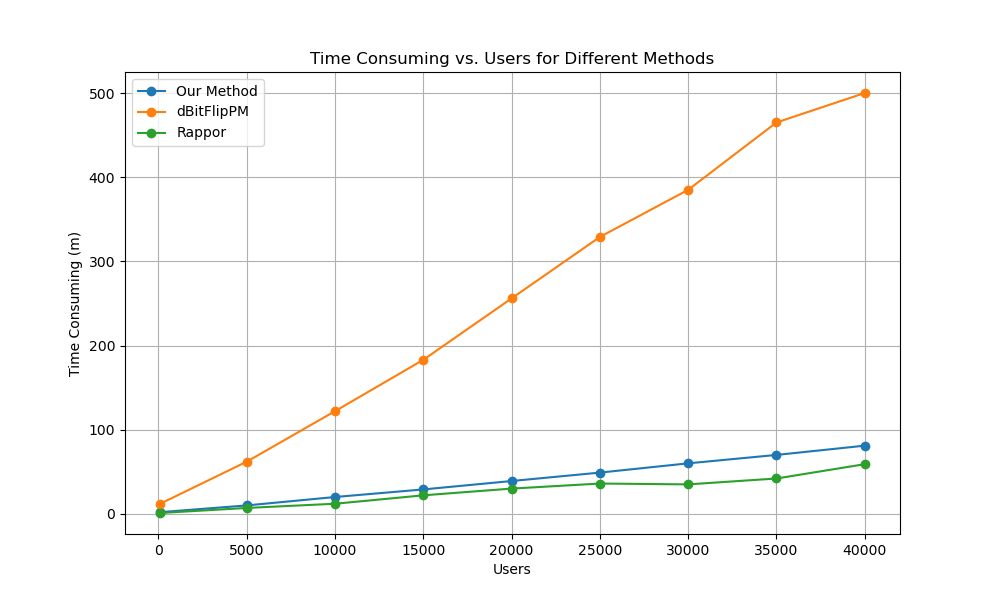
\includegraphics[width=0.9\textwidth]{figs/evaluation_usr_tim.png}
  \caption{مقایسه‌ی زمان اجرای الگورتیم پیشنهادی با دو روش رپور و دی.بیت.فلیپ.پی.اِم}
  \label{fig:usr_tim}
\end{figure}





\فصل{جمع‌بندی}

این پایان‌نامه در شش فصل به صورت جامع، چالش حفظ حریم خصوصی تفاضلی محلی را در مواجهه با دو معضل اساسی داده‌های مدرن یعنی ابعاد بالا و تغییرات مداوم، مورد بررسی قرار داده و یک راهکار ترکیبی و نوآورانه برای حل آن‌ها ارائه می‌دهد.

فصل اول، مقدمه، با تبیین اهمیت روزافزون حفاظت از داده‌ها در عصر اطلاعات، مسئله اصلی پژوهش را معرفی می‌کند. در این فصل، چالش‌های کلیدی مانند «نفرین ابعاد بالا» که منجر به افت کارایی سازوکارهای حریم خصوصی می‌شود، و مشکلات ناشی از داده‌های پویا و در حال تغییر که بودجه حریم خصوصی را به سرعت تخلیه می‌کنند، تشریح شده است. اهداف اصلی پژوهش، شامل طراحی یک ابزار سبک، کارآمد و کاربرپسند برای حفظ همزمان سودمندی و حریم خصوصی، به همراه ساختار کلی پایان‌نامه ارائه گردیده است.

فصل دوم، مفاهیم اولیه، به عنوان پایه‌ای نظری، به تشریح دقیق مفاهیم و ابزارهای ریاضی مورد استفاده در این حوزه می‌پردازد. در این بخش، تعریف رسمی حریم خصوصی تفاضلی، مفهوم کلیدی بودجه حریم خصوصی به عنوان معیاری برای سنجش سطح حفاظت، و حساسیت تابع به عنوان عاملی برای تعیین میزان نوفه لازم، مورد بحث قرار می‌گیرد. همچنین، سازوکارهای بنیادی مانند سازوکار لاپلاس برای داده‌های عددی، پاسخ تصادفی برای داده‌های دسته‌ای، و روش‌های کدگذاری و درهم‌سازی محلی به عنوان تکنیک‌های اساسی برای پیاده‌سازی در مدل محلی، به تفصیل معرفی شده‌اند.

فصل سوم، کارهای پیشین، یک مرور جامع بر ادبیات تحقیق و راهکارهای موجود برای مقابله با چالش‌های ذکر شده ارائه می‌دهد. این فصل به دو بخش اصلی تقسیم می‌شود: ابتدا، روش‌های مرتبط با داده‌های با ابعاد بالا مانند نمونه‌برداری، خوشه‌بندی، و کاهش ابعاد بررسی می‌شوند. سپس، راهکارهای ارائه‌شده برای داده‌های در حال تغییر، از جمله روش‌های مبتنی بر حفظ کردن، رند کردن و ارسال تغییرات داده تحلیل می‌گردند. این فصل با شناسایی نقاط قوت و ضعف هر روش، خلاء موجود در تحقیقات را که نیازمند یک راهکار یکپارچه است، آشکار می‌سازد.

فصل چهارم، راهکار پیشنهادی، هسته اصلی این پژوهش را تشکیل می‌دهد و یک معماری ترکیبی جدید را معرفی می‌کند که از ترکیب بهینه‌شده‌ی روش‌های پی.پی.اِم.سی و لولوها بهره می‌برد. این راهکار، داده‌های ورودی را به دو دسته ایستا (با ابعاد بالا) و پویا (در حال تغییر) تقسیم می‌کند. برای داده‌های ایستا، از تبدیل هار برای تجزیه داده به دو مؤلفه مقدار میانگین و بردار ویژه استفاده شده و هر بخش با سازوکار نوفه متناسب خود آشفته‌سازی می‌شود. برای داده‌های پویا، ابتدا از درهم‌سازی محلی برای کاهش دامنه مقادیر استفاده شده و سپس با یک سازوکار پاسخ تصادفی دائمی، حریم خصوصی در طول زمان تضمین می‌گردد. جزئیات پیاده‌سازی، از جمله نحوه بهینه‌سازی ورودی‌ها، در این فصل به طور کامل شرح داده شده است.

فصل پنجم، ارزیابی روش پیشنهادی، به سنجش عملکرد و کارایی راهکار ارائه‌شده در مقایسه با چهار روش برجسته پیشین می‌پردازد. با استفاده از مجموعه داده‌های بزرگسالان و مصنوعی سین، آزمایش‌های گسترده‌ای تحت شرایط مختلف، از جمله تغییر بودجه حریم خصوصی، افزایش ابعاد داده، و افزایش تعداد کاربران، انجام شده است. معیارهای ارزیابی شامل خطای مجذور میانگین، اختلاف توزیع احتمال و دقت تخمین شمارش بوده است.

در نهایت فصل ششم، فصل حاضر، ضمن مرور کلی بر مباحث مطرح‌شده، دستاوردهای اصلی پژوهش را خلاصه می‌کند. این فصل تأکید می‌کند که راهکار ترکیبی ارائه‌شده، یک چارچوب قدرتمند و عملی برای پیاده‌سازی حریم خصوصی تفاضلی محلی در شرایط واقعی و پیچیده است.

\قسمت{نتیجه‌گیری}

راهکار ترکیبی ارائه شده، یک رویکرد جامع و قدرتمند برای پیاده‌سازی حریم خصوصی تفاضلی محلی در شرایط معمول دنیای واقعی است. این معماری با تفکیک هوشمندانه داده‌های ایستا و پویا، بهترین تکنیک‌ها را برای هر کدام به کار می‌گیرد:

\شروع{فقرات}

\فقره تبدیل هار با موفقیت نفرین ابعاد بالا را مهار کرده و امکان جمع‌آوری داده‌های چندبعدی با کارایی بالا را فراهم می‌آورد.

\فقره روش لولوها به طور مؤثری چالش داده‌های در حال تحول را حل می‌کند و با کاهش دامنه از طریق درهم‌سازی، یک راهکار مقیاس‌پذیر با تضمین حریم خصوصی تفاضلی در طول زمان ارائه می‌دهد.

\پایان{فقرات}

پیاده‌سازی و ارزیابی این راهکار ترکیبی نشان داد که می‌توان به طور همزمان به سطح بالایی از حریم خصوصی و دقت آماری دست یافت. نتایج به‌دست‌آمده، برتری مشهود این روش را در مقایسه با راهکارهای پیشین، هم از نظر میزان خطای کمتر و هم از نظر مقیاس‌پذیری در برابر افزایش تعداد کاربران، به اثبات رساند. این موفقیت، مسیر را برای توسعه سیستم‌های تحلیل داده امن و قابل اعتماد هموارتر می‌سازد و به سازمان‌ها این امکان را می‌دهد که بدون به خطر انداختن حریم خصوصی افراد، از داده‌های ارزشمند خود بهره‌برداری کنند. در نهایت، این پژوهش گامی مهم در جهت کاربردی‌تر کردن مفاهیم حریم خصوصی تفاضلی برداشت و نشان داد که با ترکیب هوشمندانه روش‌ها، می‌توان بر پیچیده‌ترین چالش‌های این حوزه غلبه کرد.

\قسمت{کارهای آتی}

در آینده می‌توان یک منطق ریاضی برای پیدا کردن حد آستانه‌ی مناسب در آشفته‌سازی بردار ویژه یافت که توازن درستی بین حریم خصوصی و سودمندی برقرار کند. همچنین امکان تغییر الگوریتم دی.بیت.فلیپ.پی.اِم در صورتی که با همان کارایی، امنیت و سرعت بیشتری تولید شود، وجود دارد.

در نهایت باید گفت حوزه حریم خصوصی تفاضلی همچنان نیازمند تحقیق و پژوهش به منظور یافتن الگوریتم کم هزینه و کارآمد خواهد بود.





% -------------- Bibliography & Dictionary ---------------

\include{bibs/bibs}

\clearpage
\phantomsection
\addcontentsline{toc}{chapter}{واژه‌نامه}

\chapter*{واژه‌نامه}
\begin{multicols}{2}
\small

\dicalphabet{الف}
\dic{threshold}{آستانه}
\dic{perturbation}{آشفته‌سازی}
\dic{consensus}{اجماع}
\dic{probability}{احتمال}
\dic{communication}{ارتباط}
\dic{information}{اطلاعات}
\dic{safe}{امن}
\dic{transform}{انتقال}
\dic{internet of things}{اینترنت اشیاء}
\dic{high dimensions}{ابعاد بالا}

\dicalphabet{ب}
\dic{reset}{بازنشانی}
\dic{online}{برخط}
\dic{adult}{بزرگسال}
\dic{dimension}{بُعد}
\dic{optimum}{بهینه}
\dic{maximum}{بیشینه}
\dic{entropy}{بی‌نظمی}

\dicalphabet{پ}
\dic{randomize response}{پاسخ تصادفی}
\dic{query}{پرس‌و‌جو}
\dic{cover}{پوشش}
\dic{complexity}{پیچیدگی}

\dicalphabet{ت}
\dic{function}{تابع}
\dic{experimental}{تجربی}
\dic{composition}{ترکیب}
\dic{detection}{تشخیص}
\dic{intersection}{تقاطع}
\dic{approximation}{تقریب}
\dic{randomize}{تصادفی}
\dic{collision}{تصادم}
\dic{differential}{تفاضلی}
\dic{distribution}{توزیع}

\dicalphabet{چ}
\dic{density}{چگالی}

\dicalphabet{ح}
\dic{privacy}{حریم خصوصی}
\dic{sensitivity}{حساسیت}
\dic{cache}{حافظه نهان}
\dic{memoization}{حفظ کردن}
\dic{attack}{حمله}

\dicalphabet{خ}
\dic{error}{خطا}
\dic{linear}{خطی}
\dic{cluster}{خوشه}

\dicalphabet{د}
\dic{data}{داده}
\dic{outlier data}{داده‌ی پرت}
\dic{telemetry data}{داده‌ی دورسنجی}
\dic{data mining}{داده‌کاوی}
\dic{junction tree}{درخت اتصال}
\dic{evolving}{در حال تغییر}
\dic{hash}{درهم‌سازی}
\dic{doubling}{دوبرابرسازی}
\dic{binary}{دودویی}

\dicalphabet{ر}
\dic{vertex}{رأس}
\dic{formal}{رسمی}

\dicalphabet{ز}
\dic{sublinear}{زیرخطی}

\dicalphabet{س}
\dic{mechanism}{سازوکار}
\dic{time-series}{سری زمانی}
\dic{hierarchichal}{سلسه‌مراتبی}
\dic{utility}{سودمندی}

\dicalphabet{ش}
\dic{pseudocode}{شبه کد}
\dic{network}{شبکه}
\dic{counter}{شمارنده}
\dic{object}{شیء}

\dicalphabet{ط}
\dic{longitudinal}{طولی}

\dicalphabet{ع}
\dic{general}{عمومی}

\dicalphabet{غ}
\dic{dominate}{غلبه}

\dicalphabet{ف}
\dic{distance}{فاصله}
\dic{compression}{فشرده‌سازی}
\dic{space}{فضا}

\dicalphabet{ق}
\dic{deterministic}{قطعی}

\dicalphabet{ک}
\dic{efficient}{کارا}
\dic{candidate}{کاندیدا}
\dic{reduction}{کاهش}
\dic{encode}{کدگذاری}
\dic{decode}{کدگشایی}
\dic{minimum}{کمینه}

\dicalphabet{گ}
\dic{cohort}{گروه}

\dicalphabet{م}
\dic{local}{محلی}
\dic{direct}{مستقیم}
\dic{set}{مجموعه}
\dic{metric}{معیار}
\dic{mutual}{متقابل}
\dic{symmetric}{متقارن}
\dic{sequential}{متوالی}
\dic{expected}{مورد انتظار}
\dic{trade off}{موازنه}
\dic{parallel}{موازی}
\dic{average}{میانگین}

\dicalphabet{ن}
\dic{center point}{نقطه‌ی مرکزی}
\dic{noise}{نوفه}

\dicalphabet{هـ}
\dic{correlation}{همبستگی}
\dic{neighbour}{همسایه}
\dic{cost}{هزینه}

\dicalphabet{ی}
\dic{edge}{یال}
\dic{unary}{یکانی}

\end{multicols}




% -------------------- Appendices --------------------

\begin{appendix}

\فصل{مطالب تکمیلی}

مجموعه کدهای پیاده‌سازی شده برای این پروژه داخل گیتهاب\پانویس{Github} قرار گرفته است \مرجع{WoDCitekeyMisc}. به منظور اجرای الگوریتم از ابزار داکر\پانویس{Docker} استفاده شده است تا در راه‌اندازی آن تسهیل شود. به این ترتیب با داشتن سیستم عامل لیونکس\پانویس{Linux} و نصب داکر، می‌توانید به راحتی روش پیشنهادی را در محیط‌های مختلف اجرا کرده و نتایج را به صورت کامل دریافت کنید.


\end{appendix}


% -------------------- English Pages --------------------

%\newgeometry{left=3cm,right=2.5cm}

\pagestyle{empty}

% -------------------------------------------------------
%  English Abstract
% -------------------------------------------------------

\begin{latin}

\begin{center}
\textbf{Abstract}
\end{center}
\baselineskip=.8\baselineskip

Local Differential Privacy (LDP) is a leading approach for user data protection, guaranteeing privacy without needing to trust the data aggregator. This concept enables data analysis by adding noise to user data before it is sent to the aggregator. This report focuses on the challenges of maintaining LDP for high-dimensional and evolving data. Fundamental challenges in this domain include the correlation between features, increased data sensitivity, and the rapid consumption of the privacy budget, all of which can severely degrade the accuracy and efficiency of statistical analyses.
The secure application of such data is critical in areas like the Internet of Things (IoT), healthcare, and monitoring systems. This is because the data is often used for key decision-making and the development of smart services, making the preservation of user privacy throughout these processes a top priority. This report categorizes, reviews, and compares previous algorithms and works, while also presenting a novel solution to address the challenges posed by high-dimensional and evolving data.
By leveraging the Haar Transform and local hashing, this solution optimally allocates the privacy budget, thereby reducing excess noise. Furthermore, by managing and reducing the data domain, it resolves issues associated with large domains and enhances the accuracy and efficiency of the processes. Ultimately, the findings of this research provide a practical and efficient framework for analyzing high-dimensional and evolving data, which can be employed as a functional tool in various data-driven systems.

\bigskip\noindent\textbf{Keywords}:
Local Differential Privacy, Evolving Data, High-Dimensional Data, Haar Transform, Local Hashing

\end{latin}

\include{front/template/title-eng}


% -------------------- The End! --------------------

\end{document}

